\documentclass[11pt]{article}

% ===== Packages =====
\usepackage[margin=1in]{geometry}
\usepackage{amsmath, amssymb, amsthm, mathtools, bm}
\usepackage{graphicx}
\usepackage{subcaption}
\usepackage{booktabs}
\usepackage{longtable}
\usepackage{hyperref}
\usepackage{enumitem}
\usepackage{parskip}
\usepackage{float}
\usepackage{caption}
\usepackage{listings}
\usepackage{xcolor}
\usepackage{array}
\usepackage{multirow}
\usepackage{tikz}
\usetikzlibrary{shapes, arrows.meta, positioning, fit, backgrounds}

% ===== Hyperref setup =====
\hypersetup{
    colorlinks=true,
    linkcolor=blue!50!black,
    citecolor=blue!50!black,
    urlcolor=blue!70!black,
}

% ===== Theorem environments =====
\newtheorem{proposition}{Proposition}
\newtheorem{definition}{Definition}
\theoremstyle{remark}
\newtheorem{remark}{Remark}

% ===== Math macros =====
\newcommand{\SO}{\mathrm{SO}(3)}
\newcommand{\se}{\mathrm{SE}(3)}
\newcommand{\so}{\mathfrak{so}(3)}
\newcommand{\R}{\mathbb{R}}
\newcommand{\tr}{\mathrm{tr}}
\newcommand{\diag}{\mathrm{diag}}
\newcommand{\eR}{e_R}
\newcommand{\eOm}{e_\Omega}
\newcommand{\ex}{e_x}
\newcommand{\ev}{e_v}
\newcommand{\hatmap}[1]{\widehat{#1}}
\newcommand{\hatexp}[1]{({#1})^\wedge}
\newcommand{\lmin}{\lambda_{\min}}
\newcommand{\lmax}{\lambda_{\max}}

% ===== Code listing setup =====
\definecolor{codegray}{rgb}{0.95,0.95,0.95}
\definecolor{codegreen}{rgb}{0.0,0.5,0.0}
\definecolor{codepurple}{rgb}{0.58,0,0.82}
\lstset{
    backgroundcolor=\color{codegray},
    basicstyle=\ttfamily\footnotesize,
    commentstyle=\color{codegreen},
    keywordstyle=\color{blue},
    stringstyle=\color{codepurple},
    breaklines=true,
    captionpos=b,
    frame=single,
    numbers=left,
    numberstyle=\tiny\color{gray},
}

% ===== Title =====
\title{\textbf{Benchmarking Isaac Sim Fidelity for Aerial-Robotics Control\\
Using a Geometric-Controller F450 Case Study}\\[0.4em]
\large MEng Project Final Report}
\author{Zouhair Adam Hamaimou\\
Student Number: 1004891986\\[0.3em]
University of Toronto Institute for Aerospace Studies\\[0.3em]
Supervised by: Dr.~Hugh Liu}
\date{\today}

\begin{document}

% ===== Title page =====
\maketitle
\thispagestyle{empty}

\begin{abstract}
\noindent
This report investigates the fidelity of NVIDIA Isaac Sim, coupled to the Pegasus Simulator, as a development environment for aerial-robotics research. Rather than treating the geometric tracking controller of Lee et al.~\cite{Lee2010CDC} as the object of study, we use it as a fixed, theoretically well-understood instrument that produces a deterministic command stream from a known reference trajectory; tracking error can then be interpreted primarily as the result of modelling and numerical assumptions in the simulator and the F450 vehicle model rather than as a property of the controller itself. A detailed CAD model of the F450 was developed in OnShape and converted to a USD asset; a linear thrust model maps normalised throttle to rotor force; the geometric controller is implemented as a ROS\,2 node with full feed-forward terms derived analytically from the flat outputs.

We benchmark five configurations of progressively increasing modelling complexity on a single ascending elliptic-helix reference: (i) an idealised single-rigid-body block as a baseline, (ii) the F450 articulation with thrust and moment applied at the centre of mass, (iii) the F450 with per-rotor forces and a body-applied yawing moment, and (iv)--(v) the F450 vehicle model integrated by a custom ROS\,2 physics solver using fourth-order Runge--Kutta and forward Euler respectively, in place of Isaac Sim's PhysX engine. The differences between adjacent configurations isolate the contribution of each modelling assumption to the observed tracking error. The report also documents in full the geometric controller's stability theory and the analytical derivation of the desired body-frame angular velocity and acceleration, which together provide the theoretical basis for treating the controller as a known fixed instrument. The work delivers to the FSC Lab a reusable simulation pipeline and a quantitative characterisation of where Isaac Sim's modelling fidelity stands relative to a custom-integrated reference.
\end{abstract}

\newpage

% ===== Table of Contents on its own page =====
\tableofcontents
\thispagestyle{empty}
\newpage

% ============================================================
\section{Introduction}
% ============================================================

\subsection{Motivation}
The Flight Systems and Control (FSC) Lab at the University of Toronto Institute for Aerospace Studies operates an F450 research quadrotor and develops new control and estimation algorithms in NVIDIA Isaac Sim, coupled to the Pegasus Simulator. Two natural questions follow: how faithful is Isaac Sim's PhysX-backed rigid-body simulation to the physics that the algorithms will encounter on hardware, and how much of any observed discrepancy is attributable to the simulator itself versus to the user-supplied vehicle model? These cannot be answered by simply running a controller in simulation and reporting the tracking error; that error confounds controller imperfection, vehicle-model imperfection, and simulator imperfection.

This project performs a controlled experiment in which the controller and reference trajectory are held fixed and only the modelling assumptions vary. The geometric tracking controller on $\se$ of Lee et al.~\cite{Lee2010CDC} is used as the fixed instrument: it is exponentially stable on almost all of $\se$ (Propositions~\ref{prop:1}--\ref{prop:3}), is defined directly on the manifold so that singularities and sign ambiguities never enter the picture, and is fully characterised analytically. With this instrument fixed, the tracking error can be interpreted primarily as the result of modelling and numerical choices.

\subsection{Objectives}
\begin{enumerate}[label=(\roman*)]
    \item Develop a CAD-derived dynamic model of the F450 quadrotor.
    \item Implement the geometric tracking controller of \cite{Lee2010CDC} with full feed-forward terms as a fixed reference instrument.
    \item Integrate the controller into Isaac Sim through the Pegasus Simulator and a ROS\,2 backend.
    \item Benchmark Isaac Sim's modelling fidelity against an idealised baseline and a custom ROS\,2 physics solver on a single non-symmetric reference trajectory.
\end{enumerate}

\subsection{Contributions}
\begin{itemize}
    \item A CAD-derived dynamic model and a measured linear thrust curve for the F450.
    \item A self-contained treatment of the geometric tracking controller's stability analysis, including a corrected matrix bound in the complete-dynamics proof (Remark~\ref{rem:W1_tilde}).
    \item An analytical derivation of $\Omega_d$ and $\dot\Omega_d$ from the flat outputs up to snap and yaw acceleration.
    \item A control-allocation matrix consistent with the F450 rotor ordering and the Isaac Sim body-frame convention.
    \item Extensions to the Pegasus Simulator source code (jerk publishing, angular-velocity frame correction, ROS\,2 throttle backend).
    \item A five-configuration benchmark that isolates the contribution of articulation modelling, force-distribution modelling, and integrator choice to the tracking error in Isaac Sim.
\end{itemize}

\subsection{Report Structure}
Section~\ref{sec:vehicle-modelling} describes the CAD model and physical-parameter identification. Section~\ref{sec:simulation-setup} documents the Isaac Sim USD asset creation. Section~\ref{sec:geometric-control} summarises the geometric controller; the full derivation, stability proofs, and feed-forward derivation are in Appendices~\ref{app:geometric-controller} and \ref{app:feedforward}. Section~\ref{sec:implementation} details the implementation, ROS\,2 integration, and the custom physics solver. Section~\ref{sec:results} presents the benchmark. Section~\ref{sec:conclusion} concludes.

% ============================================================
\section{Vehicle Modelling}
\label{sec:vehicle-modelling}
% ============================================================

\subsection{CAD Model}
A full CAD assembly of the F450 quadrotor was built in OnShape, including the frame with landing gear, a Pixhawk flight controller, the LiPo battery, the four brushless motors, the propellers, and the wiring box. All components were modelled to scale using measurements of the physical vehicle.

\begin{figure}[H]
    \centering
    % TODO: replace with your CAD screenshot
    
\includegraphics[width=0.65\textwidth]{figures/cad_f450.png}
    \caption{OnShape CAD assembly of the F450 quadrotor used to estimate mass, centre-of-gravity location, and the diagonal inertia components.}
    \label{fig:cad}
\end{figure}

\subsection{Physical Properties}
The mass, centre-of-gravity (CoG), and diagonal inertia components of the complete assembly were estimated directly from OnShape's mass-properties tool. Because the quadrotor is nearly symmetric about the body axes, off-diagonal inertia terms are small and are assumed to be zero for the purposes of the controller.

The mass breakdown of the individual components, taken from the OnShape parts list, is given in Table~\ref{tab:mass-breakdown}. The summed total agrees with the measured total mass of the physical vehicle to within the accuracy of the kitchen-scale measurement.

\begin{table}[H]
    \centering
    \caption{Mass breakdown of the F450 components from the OnShape CAD assembly.}
    \label{tab:mass-breakdown}
    \begin{tabular}{lc}
        \toprule
        Component                               & Mass (kg) \\
        \midrule
        F450 frame with landing gear            & $0.728$ \\
        Pixhawk flight controller               & $0.104$ \\
        LiPo battery                            & $0.420$ \\
        Brushless motor (per unit, $\times 4$)  & $0.065$ \\
        Propeller (per unit, $\times 4$)        & $0.012$ \\
        Wiring box                              & $0.232$ \\
        Miscellaneous (screws, fasteners)       & $0.014$ \\
        \midrule
        \textbf{Total}                          & $\mathbf{1.806}$ \\
        \bottomrule
    \end{tabular}
\end{table}

The centre of gravity of the complete assembly coincides with the body-frame origin in the $x$--$y$ plane (i.e.\ it lies on the geometric centre of the rotor square when viewed from above). For the controller, the body-frame origin is defined to coincide with the CoG in all three axes, so no CoG offset appears in the equations of motion of Section~\ref{sec:geometric-control}. The vertical CoG height above the ground in the nominal resting pose is $0.165$~m, which is used in simulation as the initial $z$-position of the vehicle when it takes off from the ground. The overall physical parameters used by the controller are summarised in Table~\ref{tab:phys-params}.

\begin{table}[H]
    \centering
    \caption{Physical parameters of the F450 used by the controller.}
    \label{tab:phys-params}
    \begin{tabular}{llc}
        \toprule
        Symbol & Quantity & Value \\
        \midrule
        $m$         & Total mass (kg)                                & $1.806$ \\
        $J_{xx}$    & Roll inertia about the CoG (kg\,m$^2$)         & $0.016$ \\
        $J_{yy}$    & Pitch inertia about the CoG (kg\,m$^2$)        & $0.017$ \\
        $J_{zz}$    & Yaw inertia about the CoG (kg\,m$^2$)          & $0.024$ \\
        $d$         & Arm length from CoG to rotor (m)               & $0.215$ \\
        $z_0$       & Ground-to-CoG height in resting pose (m)       & $0.165$ \\
        \bottomrule
    \end{tabular}
\end{table}

\subsection{Linear Thrust-Curve Identification}
\label{sec:thrust-curve}
The Pegasus motor abstraction represents each rotor's commanded input as a normalised throttle $u_i \in [0,1]$. To close the loop between the controller (which produces forces and moments) and the simulated rotors, a mapping from $u_i$ to thrust $f_i$ is required. Bench tests of the F450 motor-propeller combination were performed and a linear least-squares fit of the form
\begin{equation}
    f_i = k_f\, u_i, \qquad k_f = 9.7237~\mathrm{N}
    \label{eq:thrust-curve}
\end{equation}
was found to capture the measured data well over the operating range used in simulation (see Figure~\ref{fig:thrust-curve}). The small nonlinearities at very low throttle are acceptable because the quadrotor typically operates around hover throttle.

\begin{figure}[H]
    \centering
    % TODO: replace with your measured thrust-curve plot
    
\includegraphics[width=0.65\textwidth]{figures/thrust_curve.png}
    \caption{Measured thrust versus normalised throttle for the F450 motor-propeller assembly, with a linear least-squares fit of slope $k_f = 9.7237~\mathrm{N}$.}
    \label{fig:thrust-curve}
\end{figure}

\subsection{Rolling Moment Coefficient}
\label{sec:moment-coefficient}
The reactive torque produced by each rotor about the body $z$-axis is modelled as a linear function of the normalised throttle:
\begin{equation}
    \tau_i = \sigma_i\, k_m\, u_i, \qquad k_m = 8\times 10^{-2}~\mathrm{N\,m},
    \label{eq:moment-curve}
\end{equation}
where $i \in \{0, 1, 2, 3\}$ indexes the rotors and $\sigma_i$ is a fixed $\pm 1$ sign that depends on the rotation direction of rotor $i$. For the F450 as configured in this project, $(\sigma_0, \sigma_1, \sigma_2, \sigma_3) = (-1, -1, +1, +1)$: rotors $0$ and $1$ spin in one direction, and rotors $2$ and $3$ spin in the opposite direction. This pattern, together with the X-arm geometry, produces a balanced reactive torque in hover and allows yaw control by differential throttling of the two groups. The resulting yaw-moment row of the allocation matrix is given in Section~\ref{sec:alloc}.

Unlike the thrust coefficient $k_f$, the value of $k_m$ used here was not identified from bench tests. It was chosen as an engineering guess of the correct order of magnitude, sufficient to obtain plausible yaw authority in simulation, and was then held fixed throughout tuning and testing. A direct measurement of $k_m$ on a torque bench is left as future work (Section~\ref{sec:future-work}); this is an important limitation of the present model, because an incorrect $k_m$ scales the yaw-moment column of $\Lambda^{-1}$ and therefore biases the yaw channel of the controller on the real hardware.

% ============================================================
\section{Simulation Environment Setup}
\label{sec:simulation-setup}
% ============================================================

The simulation stack consists of NVIDIA Isaac Sim as the physics and rendering engine, the Pegasus Simulator as the quadrotor abstraction layer, and ROS\,2 as the messaging middleware between the simulator and the controller. Importing the custom F450 asset into Isaac Sim requires producing a USD file with the correct articulation structure, rigid-body masses, and physics properties. The procedure developed during the project is documented below for reproducibility, with screenshots of each step that benefits from visual reference.

\subsection{USD File Creation Procedure}
\label{sec:usd-procedure}

The procedure below produces a USD asset of the F450 quadrotor that is compatible with the Pegasus Simulator. It is documented step-by-step because several of the gotchas discovered during this project are not apparent from the Isaac Sim documentation alone.

\subsubsection{Step 1 --- Prepare the OnShape Assembly}

\paragraph{Step 1.1.} Set the workspace units to metres using \texttt{Top left $\to$ Workspace units $\to$ Length $\to$ Metres}.

\begin{figure}[H]
    \centering
    
\includegraphics[width=0.6\textwidth]{figures/usd_steps/01_workspace_units.png}
    \caption{OnShape workspace-units window.}
    \label{fig:usd-workspace-units}
\end{figure}

\paragraph{Step 1.2.} Build a single assembly named \texttt{vehicle} in which the frame is a single part called \texttt{body}, each propeller is a separate part, and a revolute joint is defined between the \texttt{body} and each rotor. The auto-generated rotor names produced by OnShape (\texttt{rotor<1>}, \texttt{rotor<2>}, \ldots) are renamed later in Isaac Sim to match the Pegasus naming convention (Section~\ref{sec:rename-step}).

\begin{figure}[H]
    \centering
    
\includegraphics[width=0.78\textwidth]{figures/usd_steps/02_assembly_structure.png}
    \caption{OnShape assembly view of the F450, with the \texttt{body}, the four rotor parts, and the four revolute joints highlighted.}
    \label{fig:usd-assembly-structure}
\end{figure}

\paragraph{Step 1.3.} Align the assembly origin with the centre of mass of the drone.

\begin{figure}[H]
    \centering
    
\includegraphics[width=0.7\textwidth]{figures/usd_steps/03_origin_at_com.png}
    \caption{OnShape mass-properties readout showing the assembly origin coincident with the centre of mass.}
    \label{fig:usd-origin-com}
\end{figure}

\subsubsection{Step 2 --- Import into Isaac Sim}

\paragraph{Step 2.1.} Authenticate the OnShape account in a browser.

\begin{figure}[H]
    \centering
    
\includegraphics[width=0.55\textwidth]{figures/usd_steps/04_onshape_signin.png}
    \caption{OnShape browser sign-in page.}
    \label{fig:usd-onshape-signin}
\end{figure}

\paragraph{Step 2.2.} In Isaac Sim, open \texttt{File $\to$ Import from OnShape}, select the project containing the F450 assembly, and choose the \texttt{vehicle} assembly.

\begin{figure}[H]
    \centering
    
\includegraphics[width=0.7\textwidth]{figures/usd_steps/05_onshape_importer.png}
    \caption{Isaac Sim OnShape Importer with the \texttt{vehicle} assembly selected.}
    \label{fig:usd-onshape-importer}
\end{figure}

\paragraph{Step 2.3.} The importer prompts for material, mass, and tessellation settings on each part. Close this window without setting masses; the masses are assigned manually later (Step~8) once the prim hierarchy is in its final form.

\begin{figure}[H]
    \centering
    
\includegraphics[width=0.7\textwidth]{figures/usd_steps/06_importer_skip_mass.png}
    \caption{Importer parts list. Dismiss this dialog without setting masses; masses are assigned manually in Step~8.}
    \label{fig:usd-importer-skip-mass}
\end{figure}

\subsubsection{Step 3 --- Save Flattened and Re-open}

The OnShape importer produces a USD scene with a deeply nested prim hierarchy that is not directly usable by Pegasus. Saving a \emph{flattened} copy collapses the hierarchy into a form that can be edited.

\begin{figure}[H]
    \centering
    \begin{subfigure}[t]{0.46\textwidth}
        \centering
        
\includegraphics[width=\linewidth]{figures/usd_steps/07a_save_flattened.png}
        \caption{\texttt{File $\to$ Save Flattened As...}}
    \end{subfigure}
    \hfill
    \begin{subfigure}[t]{0.46\textwidth}
        \centering
        
\includegraphics[width=\linewidth]{figures/usd_steps/07b_open_flattened.png}
        \caption{Open the flattened USD file.}
    \end{subfigure}
    \caption{Saving a flattened copy and re-opening it.}
    \label{fig:usd-flatten}
\end{figure}

\subsubsection{Step 4 --- Restructure the Prim Hierarchy}

After flattening, the hierarchy appears as
\begin{center}
\texttt{/World/vehicle/vehicle/\{body, rotor, rotor\_01, \ldots, Revolute\_1, \ldots\}}.
\end{center}
The Pegasus articulation root expects the rotors to live directly underneath the vehicle prim, with each revolute joint underneath its corresponding rotor. The reorganisation below produces that structure.

\paragraph{Step 4.1.} Inspect the initial hierarchy.

\begin{figure}[H]
    \centering
    
\includegraphics[width=0.45\textwidth]{figures/usd_steps/08_hierarchy_initial.png}
    \caption{Initial Stage hierarchy after flattening.}
    \label{fig:usd-hierarchy-initial}
\end{figure}

\paragraph{Step 4.2.} Move every prim under \texttt{/World/vehicle/vehicle/} up one level into \texttt{/World/vehicle/}.

\begin{figure}[H]
    \centering
    
\includegraphics[width=0.45\textwidth]{figures/usd_steps/09_hierarchy_after_move.png}
    \caption{Stage hierarchy after promoting every child of \texttt{/World/vehicle/vehicle/} into \texttt{/World/vehicle/}. The empty inner \texttt{vehicle} prim is removed in the next step.}
    \label{fig:usd-hierarchy-after-move}
\end{figure}

\paragraph{Step 4.3.} Delete the now-empty inner \texttt{vehicle} prim, and rename \texttt{World} to \texttt{vehicle}.

\subsubsection{Step 5 --- Rename Rotors and Joints to the Pegasus Convention}
\label{sec:rename-step}

The Pegasus simulator hard-codes a per-rotor rotation-direction sign vector (default $[-1, -1, +1, +1]$, i.e.\ rotors $0$ and $1$ rotate one way and rotors $2$ and $3$ rotate the other way) and uses the rotor-prim names \texttt{rotor0}, \ldots, \texttt{rotor3} as ROS\,2 topic suffixes (\texttt{control/rotor0/ref}, etc.). The rotor names \emph{do not} therefore have to correspond to particular physical positions; what matters is that whichever rotor is named \texttt{rotor0} actually spins in the direction indicated by $\sigma_0 = -1$, and that the controller's allocation matrix (Section~\ref{sec:alloc}) is written in a way consistent with the chosen labelling.

In this project, the Pegasus default $\sigma$ vector is preserved, and the rotor names are chosen so that the rotation-direction pattern matches the F450's physical rotor layout: \texttt{rotor0} and \texttt{rotor1} are the two rotors that spin in the same direction, and likewise \texttt{rotor2} and \texttt{rotor3}. Each renamed joint inherits the index of the rotor it actuates (\texttt{joint0} actuates \texttt{rotor0}, and so on).

\begin{figure}[H]
    \centering
    \begin{subfigure}[t]{0.46\textwidth}
        \centering
        
\includegraphics[width=\linewidth]{figures/usd_steps/12a_rename_rotor.png}
        \caption{Renaming a rotor.}
    \end{subfigure}
    \hfill
    \begin{subfigure}[t]{0.46\textwidth}
        \centering
        
\includegraphics[width=\linewidth]{figures/usd_steps/12b_revolute_props.png}
        \caption{Revolute joint properties.}
    \end{subfigure}
    \caption{Renaming a rotor and inspecting a revolute joint's Body~0 / Body~1 attachment paths to identify which rotor it actuates.}
    \label{fig:usd-renaming}
\end{figure}

\paragraph{Step 5.1.} For each rotor, select it, choose \texttt{Rename}, and enter the chosen Pegasus name (\texttt{rotor0}, \ldots, \texttt{rotor3}).

\paragraph{Step 5.2.} For each revolute joint, open its property panel, read the Body~0/Body~1 paths to determine which rotor it actuates, and rename it to \texttt{jointN} where \texttt{N} is the index of that rotor.

\subsubsection{Step 6 --- Reparent Joints Under Their Rotors}

The Pegasus articulation root expects each revolute joint to live underneath the rotor it actuates. Moving the joints requires temporarily disabling Isaac Sim's instanceable flag on the affected prims.

\paragraph{Step 6.1.} For each of \texttt{body}, \texttt{rotor0}, \ldots, \texttt{rotor3}, open the property panel and uncheck \textbf{Instanceable}. This is required to allow the joints to be reparented in the next step.

\paragraph{Step 6.2.} Move each \texttt{jointN} underneath its corresponding \texttt{rotorN} prim.

\begin{figure}[H]
    \centering
    
\includegraphics[width=0.45\textwidth]{figures/usd_steps/10_hierarchy_final.png}
    \caption{Stage hierarchy after Step~6: each rotor owns its actuating joint.}
    \label{fig:usd-hierarchy-final}
\end{figure}

\subsubsection{Step 7 --- Delete the Placeholder Environment}

The flattened scene contains a default \texttt{Environment} prim (a ground plane and a dome light). It is unrelated to the vehicle articulation and must be removed before publishing the asset.

\begin{figure}[H]
    \centering
    
\includegraphics[width=0.45\textwidth]{figures/usd_steps/11_delete_environment.png}
    \caption{Deleting the auto-generated \texttt{Environment} prim.}
    \label{fig:usd-delete-environment}
\end{figure}

\subsubsection{Step 8 --- Assign Physics Properties}

\paragraph{Step 8.1.} Right-click on the top-level \texttt{vehicle} prim and choose \texttt{Add $\to$ Physics $\to$ Articulation Root}.

\paragraph{Step 8.2.} Right-click on each child Xform under \texttt{vehicle} (\texttt{body}, \texttt{rotor0}, \ldots, \texttt{rotor3}) and choose \texttt{Add $\to$ Physics $\to$ Mass}.

\begin{figure}[H]
    \centering
    \begin{subfigure}[t]{0.46\textwidth}
        \centering
        
\includegraphics[width=\linewidth]{figures/usd_steps/13_articulation_root.png}
        \caption{Articulation Root on \texttt{vehicle}.}
    \end{subfigure}
    \hfill
    \begin{subfigure}[t]{0.46\textwidth}
        \centering
        
\includegraphics[width=\linewidth]{figures/usd_steps/14_add_mass.png}
        \caption{Mass on a child Xform.}
    \end{subfigure}
    \caption{Adding physics components: an Articulation Root on \texttt{vehicle} (left), and a Mass on each child Xform (right).}
    \label{fig:usd-physics-menus}
\end{figure}

\paragraph{Step 8.3.} For each Xform that has a Mass component, open the property panel, find \textbf{Raw USD Properties}, and enter the centre of mass, the diagonal inertia, and the mass. The mass must be strictly positive.

\begin{figure}[H]
    \centering
    \begin{subfigure}[t]{0.46\textwidth}
        \centering
        
\includegraphics[width=\linewidth]{figures/usd_steps/15_mass_before.png}
        \caption{Before editing.}
    \end{subfigure}
    \hfill
    \begin{subfigure}[t]{0.46\textwidth}
        \centering
        
\includegraphics[width=\linewidth]{figures/usd_steps/16_mass_after.png}
        \caption{After editing.}
    \end{subfigure}
    \caption{Raw USD mass properties for the \texttt{body} Xform, before and after entering the CAD-derived values from Table~\ref{tab:phys-params}.}
    \label{fig:usd-mass-properties}
\end{figure}

\subsubsection{Step 9 --- Rotor Inertia: Use a Small Non-Zero Value}

For the rotors, only the diagonal inertia about the rotor's spin axis ($z$) is mechanically relevant; the other two diagonal entries are essentially zero. However, leaving the off-axis entries at exactly zero causes the Pegasus simulator to crash. The fix is to enter a small non-zero value (on the order of $10^{-7}~\mathrm{kg\,m^2}$) for the $x$- and $y$-diagonal inertia entries. When such a small value is typed into the field and the cursor leaves the field, the Raw USD Properties panel rounds the displayed value back to $0$, but the underlying USD attribute is updated correctly.

\begin{figure}[H]
    \centering
    
\includegraphics[width=0.7\textwidth]{figures/usd_steps/17_inertia_ui_gotcha.png}
    \caption{Entering $10^{-7}$ for a rotor's $x$-component diagonal inertia. The displayed value rounds back to $0$ when the field loses focus, but the underlying USD attribute is updated correctly.}
    \label{fig:usd-inertia-gotcha}
\end{figure}

\subsubsection{Step 10 --- Final Result}

The final asset, opened from the Pegasus Simulator, is shown in Figure~\ref{fig:usd-final}. It is now ready to be used in any of the five benchmark configurations of Section~\ref{sec:results}.

\begin{figure}[H]
    \centering
    
\includegraphics[width=0.75\textwidth]{figures/usd_steps/18_final_drone.png}
    \caption{The completed F450 USD asset opened from the Pegasus Simulator.}
    \label{fig:usd-final}
\end{figure}

% ============================================================
\section{Geometric Tracking Control on $\se$}
\label{sec:geometric-control}
% ============================================================

This section gives the high-level structure of the geometric tracking controller of \cite{Lee2010CDC} as it is used in this project. The full dynamics derivation, the tracking-error definitions on $\SO$, and the Lyapunov-based proofs of exponential stability and almost-global exponential attractiveness are given in Appendix~\ref{app:geometric-controller}; the reader who wants to verify any specific step in the controller design or stability analysis is referred there.

\subsection{Dynamics Model}

Let $x\in\R^3$ be the position of the centre of mass in an inertial frame, $v\in\R^3$ its velocity, $R\in\SO$ the body-to-inertial rotation matrix, and $\Omega\in\R^3$ the body-frame angular velocity. With total thrust $f\in\R$ and body-frame moment $M\in\R^3$, the equations of motion are
\begin{align}
    \dot{x} &= v, \label{eq:xdot}\\
    m\dot{v} &= mge_3 - f R e_3, \label{eq:vdot}\\
    \dot{R} &= R\hatmap{\Omega}, \label{eq:Rdot}\\
    J\dot{\Omega} + \Omega \times J\Omega &= M, \label{eq:Omdot}
\end{align}
where $e_3 = [0,0,1]^\top$ and $\hatmap{\cdot}:\R^3\to\so$ is the hat map. Equations~\eqref{eq:xdot}--\eqref{eq:Omdot} have a \emph{cascade structure}: the rotational dynamics are independent of the translational state, and the translational dynamics depend on $R$ only through $fRe_3$. The full reference-frame conventions, modelling assumptions, and the rotor-to-$(f, M)$ allocation matrix are reproduced in Appendix~\ref{app:dynamics}.

\subsection{Control Objective}
\label{sec:control-objective}

Given smooth desired trajectories $x_d(t)\in\R^3$ and a desired heading direction $\vec{b}_{1d}(t)\in S^2$, the controller is designed so that
\[
    x(t) \to x_d(t)
    \qquad \text{and} \qquad
    \mathrm{Proj}\bigl[\vec{b}_1(t)\bigr]
    \to
    \mathrm{Proj}\bigl[\vec{b}_{1d}(t)\bigr]
    \qquad
    \text{as } t \to \infty,
\]
where $\mathrm{Proj}[\,\cdot\,]$ denotes the normalised projection onto the plane orthogonal to $\vec{b}_{3d}(t)$. The reason a projection appears is that the desired thrust direction $\vec{b}_{3d}$ is dictated by the translational stage of the controller (Section~\ref{sec:controller-structure}), and there is no guarantee that $\vec{b}_{1d}$ is orthogonal to $\vec{b}_{3d}$ when the user supplies it; only the component of $\vec{b}_{1d}$ in the plane normal to $\vec{b}_{3d}$ is achievable. The projection definition is illustrated in Figure~\ref{fig:heading}.

\begin{figure}[H]
    \centering
    
\includegraphics[width=0.55\textwidth]{figures/heading_projection.png}
    \caption{Definition of the desired heading direction. The desired first body-axis $\vec{b}_{1d}$ is projected onto the plane normal to $\vec{b}_{3d}$. The intermediate axis $\vec{b}_{2d} = (\vec{b}_{3d}\times\vec{b}_{1d})/\|\vec{b}_{3d}\times\vec{b}_{1d}\|$ is computed first, from which the projected heading $\mathrm{Proj}[\vec{b}_{1d}] = \vec{b}_{2d}\times\vec{b}_{3d}$ is recovered. Figure adapted from \cite{Lee2010CDC}.}
    \label{fig:heading}
\end{figure}

\subsection{Controller Structure and Inputs}
\label{sec:controller-structure}

The controller has a two-stage cascade structure. Given smooth references $x_d(t)$ and a yaw heading $\vec{b}_{1d}(t)\in S^2$ and positive gains $k_x, k_v, k_R, k_\Omega$:

\paragraph{Translational stage.} Compute the virtual force vector
\begin{equation}
    A = -k_x e_x - k_v e_v - mg e_3 + m\ddot x_d, \qquad e_x = x - x_d,\ e_v = v - v_d,
\end{equation}
the desired thrust direction, and the total thrust
\begin{equation}
    \vec{b}_{3d} = -\frac{A}{\|A\|}, \qquad f = -A\cdot Re_3.
    \label{eq:b3d-f-summary}
\end{equation}

\paragraph{Attitude stage.} Construct the desired rotation matrix from $\vec{b}_{3d}$ and $\vec{b}_{1d}$,
\begin{equation}
    \vec{b}_{2d} = \frac{\vec{b}_{3d}\times\vec{b}_{1d}}{\|\vec{b}_{3d}\times\vec{b}_{1d}\|},\qquad
    R_d = [\vec{b}_{2d}\times\vec{b}_{3d},\ \vec{b}_{2d},\ \vec{b}_{3d}],
\end{equation}
define the attitude and angular-velocity tracking errors on $\SO$,
\begin{equation}
    e_R = \tfrac{1}{2}(R_d^\top R - R^\top R_d)^\vee,\qquad
    e_\Omega = \Omega - R^\top R_d \Omega_d,
    \label{eq:eR-eOm-summary}
\end{equation}
and apply the moment law
\begin{equation}
    M = -k_R e_R - k_\Omega e_\Omega + \Omega\times J\Omega - J(\hatmap{\Omega}R^\top R_d\Omega_d - R^\top R_d \dot\Omega_d).
    \label{eq:M-summary}
\end{equation}
The errors $e_R$ and $e_\Omega$ are derived geometrically as the gradient of an attitude-error function $\Psi(R,R_d) = \tfrac{1}{2}\tr(I - R_d^\top R)$ on $\SO$ and as the body-frame angular velocity of the relative rotation $R_d^\top R$, respectively; the full derivations are in Appendix~\ref{app:errors}. The moment law \eqref{eq:M-summary} is a nonlinear PD-with-feed-forward controller on $\SO$: when the feed-forward terms exactly cancel the gyroscopic and reference-attitude coupling, the closed-loop attitude error dynamics reduce to $J\dot e_\Omega = -k_R e_R - k_\Omega e_\Omega$.

The overall block structure of the controller is summarised in Figure~\ref{fig:controller}.

\begin{figure}[H]
    \centering
    
\includegraphics[width=0.85\textwidth]{figures/controller_structure.png}
    \caption{Controller structure. The trajectory tracking block computes the desired third body-axis $\vec{b}_{3d}$ and total thrust $f$ from the position command $x_d$. The attitude tracking block computes the moment $M$ to drive $R \to R_d$, constructed from $\vec{b}_{3d}$ and the heading command $\vec{b}_{1d}$. The state $(x, v, R, \Omega)$ is fed back to both blocks. Figure adapted from \cite{Lee2010CDC}.}
    \label{fig:controller}
\end{figure}

\subsection{Stability Properties}
\label{sec:stability-summary}

The closed-loop tracking error converges exponentially to zero from almost every initial condition in $\se$. Three propositions, proved in detail in Appendices~\ref{app:prop1}--\ref{app:prop3}, are used:

\begin{itemize}
    \item \textbf{Proposition~\ref{prop:1} (attitude exponential stability).} For $\Psi(R(0),R_d(0)) < 2$ (initial attitude error below $180^\circ$) and a sufficiently small initial angular-velocity error, the attitude error $(e_R, e_\Omega) \to 0$ exponentially. The region of attraction \emph{almost covers} $\SO$.

    \item \textbf{Proposition~\ref{prop:2} (complete-dynamics exponential stability).} For $\Psi(R(0),R_d(0)) \le \psi_1 < 1$ (initial attitude error below $90^\circ$) and a similar bound on the initial angular-velocity error, the full error $(e_x, e_v, e_R, e_\Omega) \to 0$ exponentially under suitable gain conditions.

    \item \textbf{Proposition~\ref{prop:3} (almost-global exponential attractiveness).} For $1 \le \Psi(R(0),R_d(0)) < 2$, the attitude first enters the region of attraction of Proposition~\ref{prop:2}, so exponential decay still holds eventually, with a multiplicative constant that depends on the initial condition.
\end{itemize}

The practical consequence is that, for almost every initial state on $\se$ (excluding the measure-zero set of exact $180^\circ$ attitude flips), the closed-loop tracking error decays exponentially. This makes the controller well-suited to act as a fixed reference instrument in the simulator-fidelity benchmark of Section~\ref{sec:results}: any error observed in simulation can be interpreted primarily as a property of the simulator and the vehicle model rather than of the controller.


% ============================================================
\section{Implementation}
\label{sec:implementation}
% ============================================================

\subsection{Coordinate Convention and Sign of Gravity}
\label{sec:convention}
The theoretical treatment in Section~\ref{sec:geometric-control} follows the convention of \cite{Lee2010CDC}, in which the inertial $e_3$ axis points \emph{downward}. Under this convention, gravity acts in the $+e_3$ direction, and the body-fixed $\vec{b}_3$ axis points downward (opposite to the total thrust), so the translational equation of motion reads
\begin{equation}
    m\dot v = mg e_3 - f R e_3. \tag{Lee}\label{eq:vdot-lee}
\end{equation}

Isaac Sim and the Pegasus Simulator use the opposite convention: the inertial $e_3$ axis points \emph{upward} (standard ENU/$Z$-up world frame), and the body-fixed $\vec{b}_3$ axis is defined to align with the positive thrust direction. Under this convention, gravity acts in the $-e_3$ direction, and the translational equation of motion is
\begin{equation}
    m\dot v = -mg e_3 + f R e_3. \tag{Impl}\label{eq:vdot-impl}
\end{equation}

Consequently, the virtual force vector $A$ defined in the controller has its gravity term with the \emph{opposite sign} from Lee's convention:
\begin{align}
A_{\text{Lee}}  &= -k_x e_x - k_v e_v - m g e_3 + m \ddot x_d, \label{eq:A-lee}\\
A_{\text{Impl}} &= -k_x e_x - k_v e_v + m g e_3 + m \ddot x_d. \label{eq:A-impl}
\end{align}
The desired thrust axis and thrust magnitude are also defined with opposite signs:
\[
\vec{b}_{3d}^{\text{Lee}}  = -\frac{A_{\text{Lee}}}{\|A_{\text{Lee}}\|},\qquad f_{\text{Lee}} = -A_{\text{Lee}} \cdot R e_3,
\]
\[
\vec{b}_{3d}^{\text{Impl}} = +\frac{A_{\text{Impl}}}{\|A_{\text{Impl}}\|},\qquad f_{\text{Impl}} = +A_{\text{Impl}} \cdot R e_3.
\]
These are the expressions used in the Python implementation (\texttt{geometric\_control.py}) and in the feed-forward derivation of Section~\ref{sec:feedforward}.

\paragraph{Why the stability proofs still apply.} The change between \eqref{eq:vdot-lee} and \eqref{eq:vdot-impl} is purely a choice of world-frame $z$-axis orientation; it is equivalent to the coordinate transformation $e_3 \mapsto -e_3$ (with a corresponding re-orientation of $R$). Since the closed-loop error dynamics of Proposition~\ref{prop:1} reduce to $J\dot e_\Omega = -k_R e_R - k_\Omega e_\Omega$ independently of the translational dynamics, and the translational error dynamics in Proposition~\ref{prop:2} reduce (in Step 2) to $m\dot e_v = -k_x e_x - k_v e_v - X$ where all the frame-dependent constants have cancelled out, the coordinate flip does not enter any of the Lyapunov inequalities. All sign changes are self-consistent: the $-mg e_3$ term in \eqref{eq:vdot-impl}, the $+mg e_3$ term in \eqref{eq:A-impl}, the $+$ sign in $\vec{b}_{3d}^{\text{Impl}}$, and the $+$ sign in $f_{\text{Impl}}$ together leave the closed-loop error dynamics unchanged. Propositions~\ref{prop:1}--\ref{prop:3} therefore apply verbatim to the implemented controller, with the understanding that $e_3$ and $R$ in the proofs are replaced by their $Z$-up-convention counterparts.

For the remainder of Section~\ref{sec:implementation}, all equations follow the implementation (Isaac Sim / $Z$-up) convention.

\subsection{Control Allocation for the F450}
\label{sec:alloc}
The F450 rotors (indexed $i \in \{0, 1, 2, 3\}$) are arranged in an X-configuration. Using the linear thrust and moment models from Section~\ref{sec:thrust-curve} and Section~\ref{sec:moment-coefficient}, the allocation from normalised throttles $u = [u_0, u_1, u_2, u_3]^\top$ to $(f, M_1, M_2, M_3)$ is
\begin{equation}
    \begin{bmatrix} f \\ M_1 \\ M_2 \\ M_3 \end{bmatrix}
    =
    \underbrace{
    \begin{bmatrix}
        k_f & k_f & k_f & k_f \\
       -\frac{k_f d}{\sqrt{2}} &  \frac{k_f d}{\sqrt{2}} &  \frac{k_f d}{\sqrt{2}} & -\frac{k_f d}{\sqrt{2}} \\
       -\frac{k_f d}{\sqrt{2}} &  \frac{k_f d}{\sqrt{2}} & -\frac{k_f d}{\sqrt{2}} &  \frac{k_f d}{\sqrt{2}} \\
       -k_m & -k_m & k_m & k_m
    \end{bmatrix}}_{\Lambda}
    \begin{bmatrix} u_0 \\ u_1 \\ u_2 \\ u_3 \end{bmatrix}.
\end{equation}
The yaw-moment row $[-k_m, -k_m, +k_m, +k_m]$ reflects the rotation-direction pattern $(\sigma_0, \sigma_1, \sigma_2, \sigma_3) = (-1, -1, +1, +1)$ established in Section~\ref{sec:moment-coefficient}. The controller outputs $(f, M)$ via \eqref{eq:b3d-f-summary}, \eqref{eq:M-summary}, which are inverted by $\Lambda^{-1}$ (computed once at initialisation) to obtain the per-rotor normalised throttles. The pair $(\Lambda, \Lambda^{-1})$ is verified numerically against $\Lambda \Lambda^{-1} = I$ at start-up.

\subsection{Feed-Forward Desired Angular Velocity and Acceleration}
\label{sec:feedforward}

The moment law \eqref{eq:M-summary} requires the desired body-frame angular velocity $\Omega_d$ and acceleration $\dot\Omega_d$ as feed-forward terms. Rather than numerically differentiating the desired attitude---which amplifies noise---these are derived analytically from the flat outputs $x_d(t)$ and $\psi_d(t)$ and their derivatives up to snap and yaw-acceleration, following the differential-flatness approach of Mellinger and Kumar~\cite{Mellinger2011}.

The full derivation is given in Appendix~\ref{app:feedforward}. The high-level computation chain is:

\begin{enumerate}[label=(\roman*), leftmargin=*]
    \item Compute $A, \dot A, \ddot A$ from the controller errors and the flat-output derivatives ($a_d, j_d, s_d$).
    \item Apply a normalisation lemma to obtain $b_{3d}$ and its first two time derivatives from $A$.
    \item Differentiate the yaw heading vector $c = [\cos\psi_d, \sin\psi_d, 0]^\top$ twice to get $\dot c, \ddot c$.
    \item Form $r = b_{3d}\times c$ and obtain $b_{2d}, \dot b_{2d}, \ddot b_{2d}$ via the same normalisation lemma.
    \item Form $b_{1d} = b_{2d}\times b_{3d}$ and obtain $\dot b_{1d}, \ddot b_{1d}$ by the product rule.
    \item Recover $\Omega_d$ and $\dot\Omega_d$ as
    \begin{equation}
        \Omega_d =
        \begin{bmatrix} b_{3d}^\top\dot b_{2d} \\ b_{1d}^\top\dot b_{3d} \\ b_{2d}^\top\dot b_{1d} \end{bmatrix},
        \qquad
        \dot\Omega_d =
        \begin{bmatrix} \dot b_{3d}^\top\dot b_{2d} + b_{3d}^\top\ddot b_{2d} \\ \dot b_{1d}^\top\dot b_{3d} + b_{1d}^\top\ddot b_{3d} \\ \dot b_{2d}^\top\dot b_{1d} + b_{2d}^\top\ddot b_{1d} \end{bmatrix}.
        \label{eq:omega-d-summary}
    \end{equation}
\end{enumerate}

The derivation assumes $\|A\| \neq 0$ and $\|b_{3d}\times c\| \neq 0$. The first fails only when the controller commands exactly zero net force; the second occurs when the commanded body-$z$ axis becomes horizontal, i.e.\ at a $90^\circ$ pitch or roll attitude. Both are guarded in the implementation by small numerical thresholds with safe fall-backs.
\subsection{Pegasus Simulator Modifications}
The Pegasus Simulator required three source modifications to support the controller:
\begin{enumerate}
    \item \textbf{Jerk output.} The simulator now publishes body-frame linear jerk $j = \dot a$, required by the $\ddot A$ computation in Section~\ref{sec:feedforward}.
    \item \textbf{Angular velocity reference frame.} The original simulator published angular velocity expressed in the world frame while mislabelling it as body-frame. This was corrected so that the published $\Omega$ matches the definition used in \eqref{eq:Rdot}.
    \item \textbf{ROS\,2 control backend.} A backend was added that subscribes to per-rotor normalised throttle commands on the ROS\,2 topic \texttt{control/rotor\{i\}/ref} and applies them directly to the simulated rotors.
\end{enumerate}

\subsection{Custom ROS\,2 Physics Solver}
\label{sec:custom-solver}
For the integrator-comparison experiments in Section~\ref{sec:results}, a separate ROS\,2 node was developed that replaces Isaac Sim's PhysX engine entirely with a hand-written rigid-body integrator. The node subscribes to the same per-rotor throttle topics as the Pegasus backend, evaluates the F450 dynamics \eqref{eq:xdot}--\eqref{eq:Omdot} using the same mass and inertia parameters as the Isaac Sim asset (Table~\ref{tab:phys-params}), advances the state by one time-step using either fourth-order Runge--Kutta (RK4) or forward Euler integration at the same $250$~Hz rate as the controller, and publishes the new state on the standard \texttt{state/*} topics. In these experiments Isaac Sim is not running at all; the custom node is the sole source of physics, providing a controlled comparison between the simulator's commercial-grade integrator and a transparent, fully-specified textbook integrator on identical inputs.

\subsection{ROS\,2 System Architecture}
\label{sec:ros2-architecture}

The closed-loop pipeline runs in two slightly different topologies depending on whether the experiment uses Isaac Sim as the physics engine (E1, E2, E3) or the custom ROS\,2 solver (E4, E5). Both topologies share the same controller and trajectory-publisher nodes; they differ only in what supplies and consumes the rotor commands. The two variants are shown in Figures~\ref{fig:block-diagram-pegasus} and \ref{fig:block-diagram-custom}. Arrows are labelled in standard control-theory notation: $\mathbf{x}$ for the measured vehicle state, $\mathbf{x}_d$ for the reference trajectory, $\mathbf{u}$ for the per-rotor commands, and $f, M$ for the lumped total thrust and body-frame moment that the controller also publishes (used by Pegasus only in the lumped-input experiments E1 and E2). Each label corresponds to one or more ROS\,2 topics, listed in Table~\ref{tab:topic-bundles}. All ROS\,2 nodes run at $250$~Hz, matched to the Isaac Sim physics step in variant A and to the custom-solver step in variant B.

\subsubsection{Variant A: Pegasus + Isaac Sim (E1, E2, E3)}

In this variant, Isaac Sim is the physics engine and the Pegasus Simulator backend bridges between Isaac Sim's internal state and the ROS\,2 topic graph. Pegasus reads the vehicle state from Isaac Sim through the Dynamic Control Python interface (not ROS\,2) and republishes it on the state-bundle topics. Conversely, the rotor commands received on ROS\,2 are converted by Pegasus into the appropriate forces and moments and applied to Isaac Sim through the same Python interface.

\begin{figure}[H]
\centering
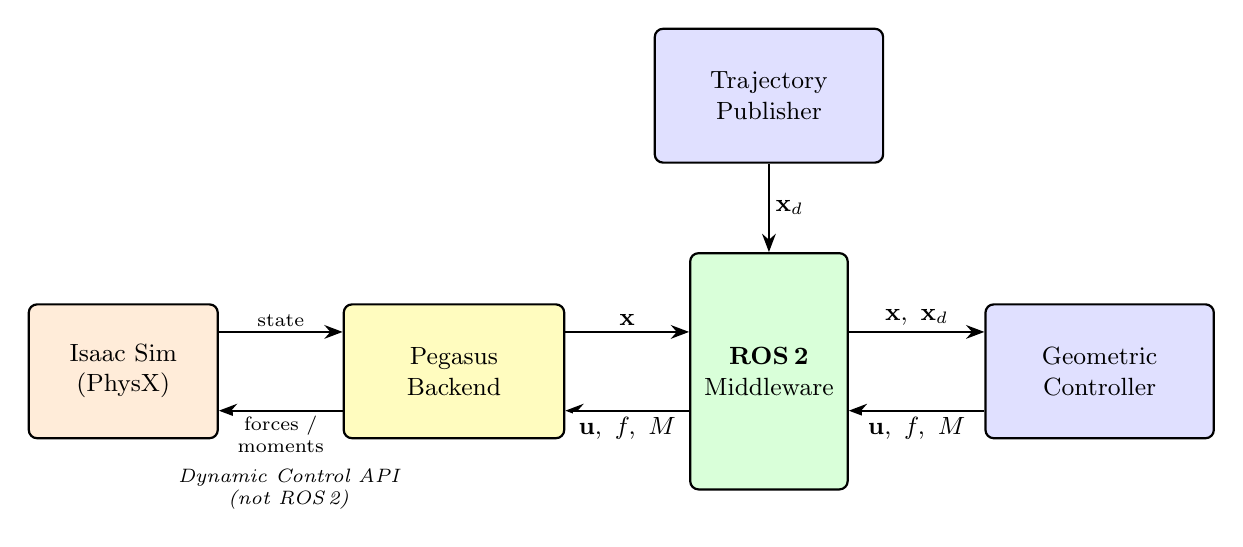
\begin{tikzpicture}[
    font=\small,
    sim/.style={draw, thick, minimum height=1.7cm, minimum width=2.4cm, align=center,
                fill=orange!15, rounded corners=3pt},
    backend/.style={draw, thick, minimum height=1.7cm, minimum width=2.8cm, align=center,
                    fill=yellow!25, rounded corners=3pt},
    ros2/.style={draw, thick, minimum height=3cm, minimum width=2cm, align=center,
                 fill=green!15, rounded corners=3pt},
    pynode/.style={draw, thick, minimum height=1.7cm, minimum width=2.9cm, align=center,
                   fill=blue!12, rounded corners=3pt},
    arr/.style={->, >=Stealth, thick},
    elab/.style={font=\small, align=center, inner sep=2pt, fill=white},
    nlab/.style={font=\scriptsize, align=center, inner sep=1.5pt, fill=white}
]

\node[sim]     (isaac)   at (0, 0)    {Isaac Sim\\(PhysX)};
\node[backend] (backend) at (4.2, 0)  {Pegasus\\Backend};
\node[ros2]    (ros2)    at (8.2, 0)  {\textbf{ROS\,2}\\Middleware};
\node[pynode]  (ctrl)    at (12.4, 0) {Geometric\\Controller};

\node[pynode]  (traj)    at (8.2, 3.5)  {Trajectory\\Publisher};

% Isaac Sim <-> Pegasus Backend (Dynamic Control API, not ROS)
\draw[arr] ([yshift=5mm]isaac.east) -- node[above, nlab]{state}
    ([yshift=5mm]backend.west);
\draw[arr] ([yshift=-5mm]backend.west) -- node[below, nlab]{forces /\\moments}
    ([yshift=-5mm]isaac.east);
\node[font=\scriptsize\itshape, align=center] at (2.1, -1.5) {Dynamic Control API\\(not ROS\,2)};

% Pegasus Backend <-> ROS 2
\draw[arr] ([yshift=5mm]backend.east) -- node[above, elab]{$\mathbf{x}$}
    ([yshift=5mm]ros2.west);
\draw[arr] ([yshift=-5mm]ros2.west) -- node[below, elab]{$\mathbf{u},\ f,\ M$}
    ([yshift=-5mm]backend.east);

% ROS 2 <-> Geometric Controller
\draw[arr] ([yshift=5mm]ros2.east) -- node[above, elab]{$\mathbf{x},\ \mathbf{x}_d$}
    ([yshift=5mm]ctrl.west);
\draw[arr] ([yshift=-5mm]ctrl.west) -- node[below, elab]{$\mathbf{u},\ f,\ M$}
    ([yshift=-5mm]ros2.east);

% Trajectory Publisher --> ROS 2
\draw[arr] (traj.south) -- node[right, elab]{$\mathbf{x}_d$} (ros2.north);

\end{tikzpicture}
\caption{Variant~A architecture (E1, E2, E3).}
\label{fig:block-diagram-pegasus}
\end{figure}

The exact translation that the Pegasus backend performs depends on which experiment is running:

\begin{itemize}
    \item \textbf{E1, E2 (lumped $(f,M)$).} Pegasus subscribes to the controller's $f$ and $M$ topics and applies them at the body's CoG.
    \item \textbf{E3 (distributed).} Pegasus subscribes to the four rotor-throttle topics $\mathbf{u}$, converts each one to a per-rotor force using the thrust curve of \eqref{eq:thrust-curve}, applies each force to the corresponding rotor link, and applies only the reactive yawing moment $M_z$ to the body.
\end{itemize}

The geometric controller publishes both $\mathbf{u}$ and $(f, M)$ in all three experiments; Pegasus only reads whichever is appropriate for the current configuration.

\subsubsection{Variant B: Custom Physics Solver (E4, E5)}

In this variant, Isaac Sim is not running. A custom ROS\,2 node integrates the rigid-body dynamics \eqref{eq:xdot}--\eqref{eq:Omdot} (RK4 in E4, forward Euler in E5) directly inside ROS\,2 and publishes the integrated state on the same state-bundle topics that Pegasus would have used in variant~A. Because the custom node receives per-rotor commands and produces a state, it functions as a one-block replacement for the entire (Pegasus, Isaac Sim) pair. The geometric controller and trajectory publisher are unchanged.

\begin{figure}[H]
\centering
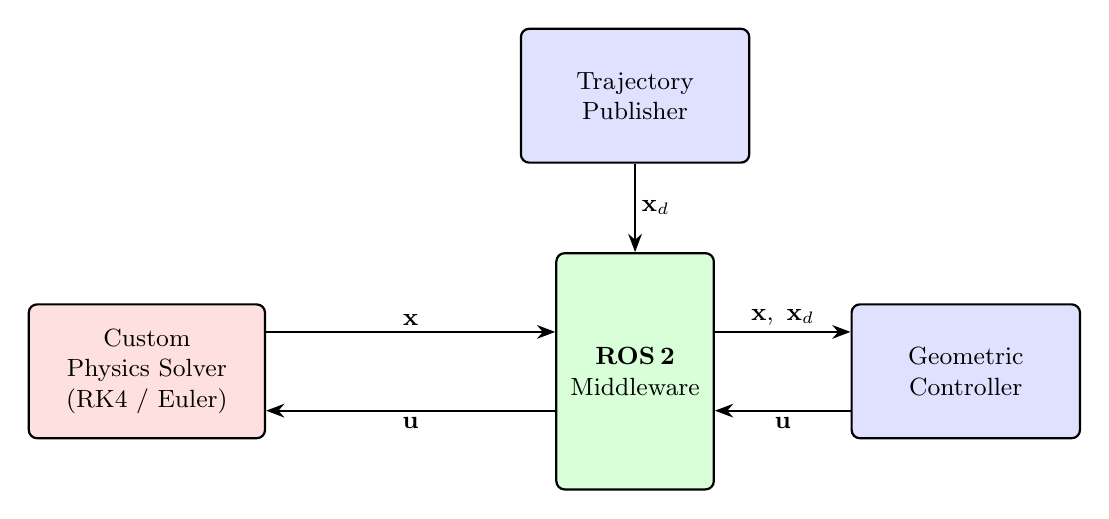
\begin{tikzpicture}[
    font=\small,
    custom/.style={draw, thick, minimum height=1.7cm, minimum width=3.0cm, align=center,
                   fill=red!12, rounded corners=3pt},
    ros2/.style={draw, thick, minimum height=3cm, minimum width=2cm, align=center,
                 fill=green!15, rounded corners=3pt},
    pynode/.style={draw, thick, minimum height=1.7cm, minimum width=2.9cm, align=center,
                   fill=blue!12, rounded corners=3pt},
    arr/.style={->, >=Stealth, thick},
    elab/.style={font=\small, align=center, inner sep=2pt, fill=white}
]

\node[custom]  (solver)  at (2.0, 0)  {Custom\\Physics Solver\\(RK4 / Euler)};
\node[ros2]    (ros2)    at (8.2, 0)  {\textbf{ROS\,2}\\Middleware};
\node[pynode]  (ctrl)    at (12.4, 0) {Geometric\\Controller};

\node[pynode]  (traj)    at (8.2, 3.5)  {Trajectory\\Publisher};

% Custom Solver <-> ROS 2
\draw[arr] ([yshift=5mm]solver.east) -- node[above, elab]{$\mathbf{x}$}
    ([yshift=5mm]ros2.west);
\draw[arr] ([yshift=-5mm]ros2.west) -- node[below, elab]{$\mathbf{u}$}
    ([yshift=-5mm]solver.east);

% ROS 2 <-> Geometric Controller
\draw[arr] ([yshift=5mm]ros2.east) -- node[above, elab]{$\mathbf{x},\ \mathbf{x}_d$}
    ([yshift=5mm]ctrl.west);
\draw[arr] ([yshift=-5mm]ctrl.west) -- node[below, elab]{$\mathbf{u}$}
    ([yshift=-5mm]ros2.east);

% Trajectory Publisher --> ROS 2
\draw[arr] (traj.south) -- node[right, elab]{$\mathbf{x}_d$} (ros2.north);

\end{tikzpicture}
\caption{Variant~B architecture (E4, E5).}
\label{fig:block-diagram-custom}
\end{figure}

\begin{table}[H]
    \centering
    \caption{ROS\,2 topics carried by each arrow-symbol of Figures~\ref{fig:block-diagram-pegasus} and \ref{fig:block-diagram-custom}. All topics are namespaced under \texttt{/uav\_0/}, with the namespace path given once per group beneath the symbol.}
    \label{tab:topic-bundles}
    \footnotesize
    \renewcommand{\arraystretch}{1.2}
    \begin{tabular}{@{}p{1.6cm} p{3.6cm} p{8.5cm}@{}}
        \toprule
        \textbf{Symbol} & \textbf{Topic} & \textbf{Description} \\
        \midrule
        \multicolumn{3}{@{}l}{\textbf{$\mathbf{x}$} \quad namespace: \texttt{state/}} \\
        \addlinespace[0.2em]
        & \texttt{pose}            & World-frame pose (position + orientation) of the body. \\
        & \texttt{twist}           & Body-frame linear and angular velocity. \\
        & \texttt{twist\_inertial} & World-frame linear and angular velocity. \\
        & \texttt{accel}           & Body-frame linear and angular acceleration. \\
        & \texttt{jerk}            & Body-frame linear jerk $\dot a$, used by the $\ddot A$ feed-forward. \\
        \midrule
        \multicolumn{3}{@{}l}{\textbf{$\mathbf{x}_d$} \quad namespace: \texttt{trajectory/desired/}} \\
        \addlinespace[0.2em]
        & \texttt{position}          & Reference position $x_d(t)$. \\
        & \texttt{velocity}          & Reference velocity $\dot x_d(t)$. \\
        & \texttt{acceleration}      & Reference acceleration $\ddot x_d(t) = a_d$. \\
        & \texttt{jerk}              & Reference jerk $\dddot x_d(t) = j_d$, for $\dot A$. \\
        & \texttt{snap}              & Reference snap $\ddddot x_d(t) = s_d$, for $\ddot A$. \\
        & \texttt{yaw}               & Reference yaw angle $\psi_d(t)$. \\
        & \texttt{yaw\_rate}         & Reference yaw rate $\dot\psi_d(t)$. \\
        & \texttt{yaw\_acceleration} & Reference yaw acceleration $\ddot\psi_d(t)$. \\
        \midrule
        \multicolumn{3}{@{}l}{\textbf{$\mathbf{u}$} \quad namespace: \texttt{control/}} \\
        \addlinespace[0.2em]
        & \texttt{rotor0/ref} & Normalised throttle command for rotor 0. \\
        & \texttt{rotor1/ref} & Normalised throttle command for rotor 1. \\
        & \texttt{rotor2/ref} & Normalised throttle command for rotor 2. \\
        & \texttt{rotor3/ref} & Normalised throttle command for rotor 3. \\
        \midrule
        \multicolumn{3}{@{}l}{\textbf{$f$, $M$} \quad namespace: \texttt{control/output/}} \\
        \addlinespace[0.2em]
        & \texttt{f} & Total thrust commanded by the controller (used by Pegasus in E1, E2). \\
        & \texttt{M} & Body-frame moment commanded by the controller (used by Pegasus in E1, E2). \\
        \bottomrule
    \end{tabular}
\end{table}

\subsection{Controller Parameter Tuning}
Separate gains were used for the yaw axis so that the yaw response could be tuned independently of the roll/pitch response. The gains used for all simulation results in Section~\ref{sec:results} are listed in Table~\ref{tab:gains}. The outer-loop position gains were tuned first with an approximate damping ratio of $\zeta \approx 0.7$, then the inner-loop attitude gains were chosen to give a roughly $10\!:\!1$ bandwidth separation. The yaw gains are smaller because yaw tracking is less time-critical and the $z$-axis has a larger inertia.

\begin{table}[H]
    \centering
    \caption{Controller gains used for all trajectory tests.}
    \label{tab:gains}
    \begin{tabular}{lcl}
        \toprule
        Parameter        & Value  & Description \\
        \midrule
        $k_x$            & $1.0$  & Position gain \\
        $k_v$            & $1.7$  & Velocity gain \\
        $k_R$            & $1.5$  & Roll/pitch attitude gain \\
        $k_\Omega$       & $0.4$  & Roll/pitch rate gain \\
        $k_{R,\psi}$     & $1.0$  & Yaw attitude gain \\
        $k_{\Omega,\psi}$& $0.35$ & Yaw rate gain \\
        Publish rate     & $250$~Hz & Control loop frequency \\
        \bottomrule
    \end{tabular}
\end{table}

% ============================================================
\section{Benchmark Results}
\label{sec:results}
% ============================================================

\subsection{Experimental Design}
\label{sec:experimental-design}

The benchmark holds the geometric controller (Section~\ref{sec:geometric-control}) and the reference trajectory fixed across all experiments and varies only the configuration of the simulated body and physics engine. Five configurations are tested, listed in order of increasing modelling complexity in Table~\ref{tab:experiments}.

\begin{table}[H]
    \centering
    \caption{Benchmark configurations used in the fidelity study.}
    \label{tab:experiments}
    \footnotesize
    \renewcommand{\arraystretch}{1.18}
    \setlength{\tabcolsep}{5pt}
    \begin{tabular}{@{}p{0.7cm} p{3.0cm} p{5.6cm} p{3.0cm}@{}}
        \toprule
        \textbf{ID} & \textbf{Body model} & \textbf{Forces / moments applied} & \textbf{Physics integrator} \\
        \midrule
        E1 & Single rigid body
           & $(f, M)$ applied at the CoG
           & Isaac Sim PhysX \\
        E2 & F450 articulation
           & $(f, M)$ applied at body
           & Isaac Sim PhysX \\
        E3 & F450 articulation
           & Per-rotor forces on rotor links + $M_z$ on body
           & Isaac Sim PhysX \\
        E4 & F450 rigid body \newline (parameters only)
           & Per-rotor forces + $M_z$ on body
           & Custom ROS\,2 RK4 \\
        E5 & F450 rigid body \newline (parameters only)
           & Per-rotor forces + $M_z$ on body
           & Custom forward Euler \\
        \bottomrule
    \end{tabular}
    \vspace{0.3em}
    \parbox{0.95\textwidth}{\footnotesize
    The geometric controller, controller gains (Table~\ref{tab:gains}), and reference trajectory are identical across all five configurations.}
\end{table}

The purpose of each configuration, and the modelling effect that is isolated by comparing it against the previous one in the table, is summarised below.

\begin{itemize}
    \item \textbf{E1 (Ideal block)} is the purest test of the geometric controller in Isaac Sim. The body is a single rigid block with the F450's mass and inertia, and the controller applies its computed thrust and moment directly at the CoG. There is no rotor articulation, no force-distribution model, no thrust-curve mapping. Any tracking error here is attributable to the controller, the trajectory, and Isaac Sim's integrator alone. This is the baseline.

    \item \textbf{E2 (F450 lumped)} replaces the block with the full F450 articulation (frame, four rotor links, four revolute joints) but still applies the resultant $(f, M)$ at the body's CoG. The difference E2$-$E1 isolates the effect of articulating the body into a multi-link rigid system, even when the same net force and moment are applied.

    \item \textbf{E3 (F450 distributed)} applies the four computed per-rotor forces directly to the four rotor links via the allocation matrix of Section~\ref{sec:alloc}, and applies only the reactive yawing moment $M_z$ to the body. This is the most physically faithful Isaac Sim configuration considered in this work. The difference E3$-$E2 isolates the effect of distributing the forces across the rotor links rather than lumping them at the CoG.

    \item \textbf{E4 (Custom RK4)} replaces Isaac Sim's PhysX integrator with the custom ROS\,2 solver of Section~\ref{sec:custom-solver}, integrating \eqref{eq:xdot}--\eqref{eq:Omdot} with fourth-order Runge--Kutta at $250$~Hz. The vehicle parameters are identical to E3. The difference E4$-$E3 isolates the effect of the integrator: PhysX (commercial, contact-aware, optimised) versus a textbook RK4 with full insight into every step.

    \item \textbf{E5 (Custom Euler)} is identical to E4 except that the integrator is forward Euler. The difference E5$-$E4 isolates the effect of integrator order on a $250$~Hz controller: a high-order method versus the lowest-order method that still produces stable trajectories.
\end{itemize}

\subsection{Reference Trajectory}
The benchmark uses an ascending elliptic helix as the single reference trajectory:
\begin{align}
    x_d(t) &= a\sin(\omega t), \\
    y_d(t) &= b\bigl(1 - \cos(\omega t)\bigr), \\
    z_d(t) &= z_0 + v_z t, \\
    \psi_d(t) &= \omega t,
\end{align}
with $a = 1$~m, $b = 2$~m, $\omega = 0.5$~rad/s, $v_z = 0.1$~m/s, and $z_0 = 0.165$~m corresponding to the resting CoG height of the vehicle (Section~\ref{sec:vehicle-modelling}). The trajectory exercises all four controllable degrees of freedom of the quadrotor: $x$ and $y$ trace an ellipse of unequal semi-axes (so the lateral acceleration is not symmetric in the body frame), $z$ ramps linearly upward, and the yaw $\psi$ rotates continuously. It runs for three full revolutions (duration $\approx 37.7$~s), long enough that any unstable mode in any of the five configurations would have time to grow visibly.

\subsection{Metrics}
\label{sec:metrics}

The natural error variables for the benchmark are those that already appear in the controller and its stability analysis (Section~\ref{sec:geometric-control} and Appendix~\ref{app:geometric-controller}): the position error $e_x = x - x_d$ and velocity error $e_v = v - v_d$, and the attitude and angular-velocity errors on $\SO$,
\begin{equation}
    e_R = \tfrac{1}{2}\bigl(R_d^\top R - R^\top R_d\bigr)^\vee,
    \qquad
    e_\Omega = \Omega - R^\top R_d \Omega_d.
\end{equation}
The aggregate metrics reported per experiment are summarised in Table~\ref{tab:metrics}.

\begin{table}[H]
    \centering
    \caption{Aggregate tracking metrics computed for each experiment. RMS is taken over the full trajectory duration; the maximum is over the same window after the initial $0.5$~s ramp-up transient.}
    \label{tab:metrics}
    \begin{tabular}{lll}
        \toprule
        Metric & Symbol & Definition \\
        \midrule
        RMS position error           & $\mathrm{RMS}_{e_x}$        & $\sqrt{\tfrac{1}{N}\sum_k \|e_x(t_k)\|^2}$ \\
        Max position error           & $\max\|e_x\|$               & $\max_k \|e_x(t_k)\|$ \\
        RMS velocity error           & $\mathrm{RMS}_{e_v}$        & $\sqrt{\tfrac{1}{N}\sum_k \|e_v(t_k)\|^2}$ \\
        RMS attitude error           & $\mathrm{RMS}_{e_R}$        & $\sqrt{\tfrac{1}{N}\sum_k \|e_R(t_k)\|^2}$ \\
        Max attitude error           & $\max\|e_R\|$               & $\max_k \|e_R(t_k)\|$ \\
        RMS angular-velocity error   & $\mathrm{RMS}_{e_\Omega}$   & $\sqrt{\tfrac{1}{N}\sum_k \|e_\Omega(t_k)\|^2}$ \\
        \bottomrule
    \end{tabular}
\end{table}

\subsection{Results}
\label{sec:results-overlays}

All plots that follow are overlays in which the five experiments E1--E5 and the reference signal share the same axes. The plots in this subsection constitute the main-report set; the per-axis velocity, acceleration, angular-rate, and angular-acceleration breakdowns, together with per-axis attitude and angular-velocity error components, are deferred to Appendix~\ref{app:plot-bank}. The numerical summary is in Table~\ref{tab:metrics-summary}; this subsection describes what is visible in the plots, and Section~\ref{sec:results-discussion} draws the conclusions.

\subsubsection{3D Trajectory and Per-Axis Position Tracking}

\begin{figure}[H]
    \centering
    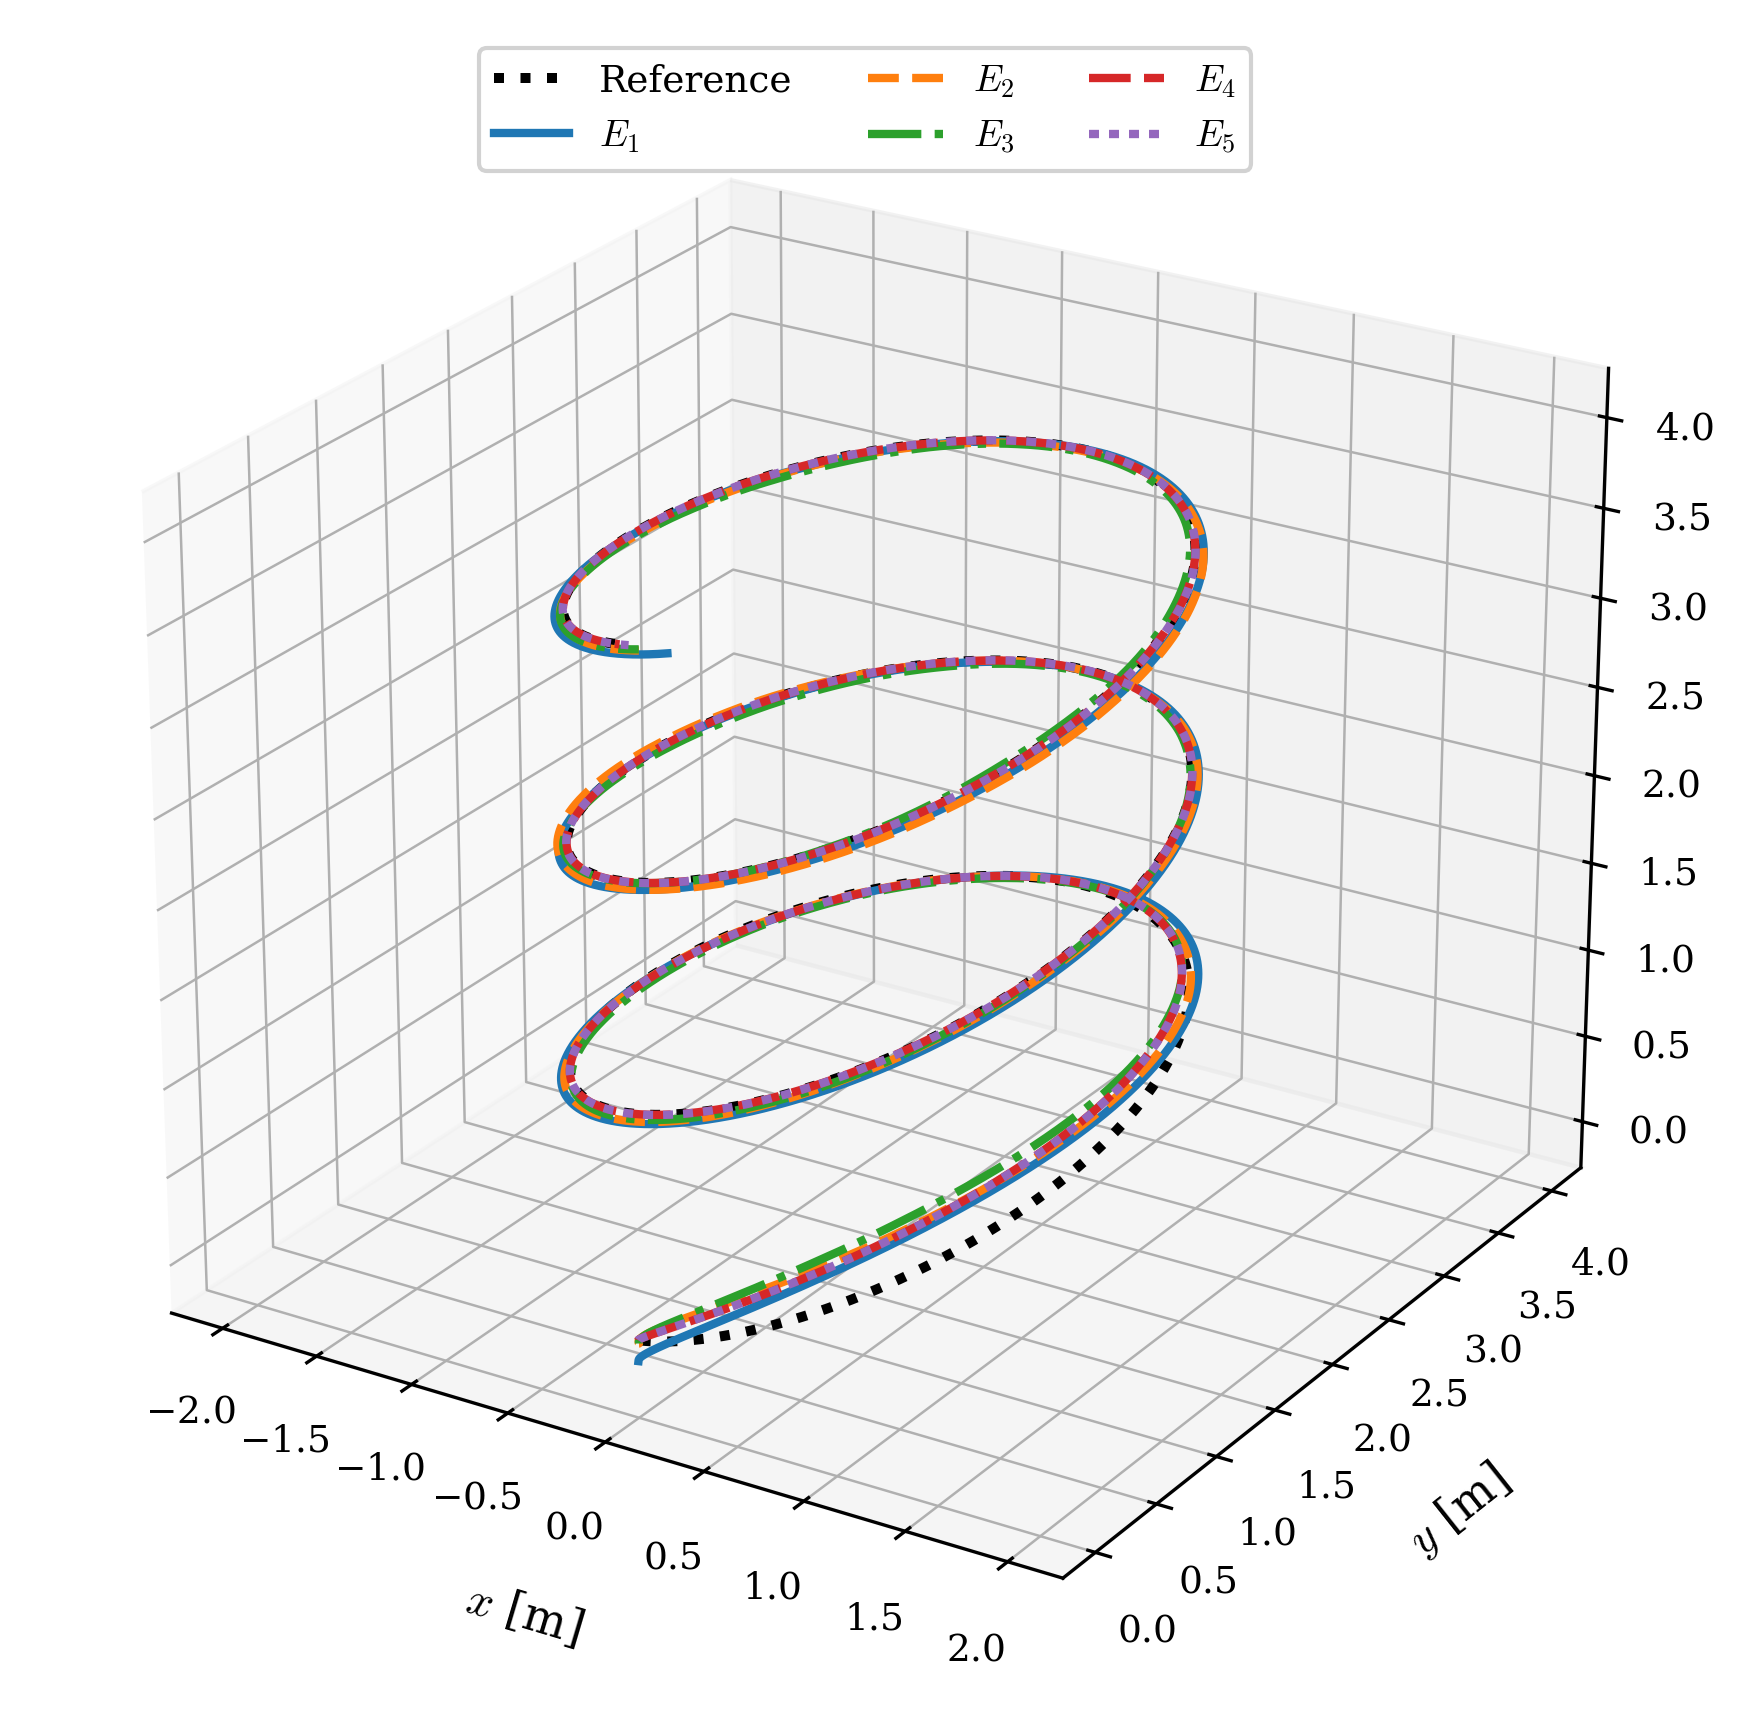
\includegraphics[width=0.72\textwidth]{experiment_plots/path_xyz_3d.png}
    \caption{3D path traced by the vehicle in each of the five configurations, overlaid against the reference helix.}
    \label{fig:overlay-3d}
\end{figure}

The five 3D paths are visually indistinguishable except very near the start, where E1 is briefly visible underneath the others as it trails the rising helix; the differences between experiments are best seen in the per-axis tracking plots and in the error norms.

\begin{figure}[H]
    \centering
    \begin{subfigure}{\textwidth}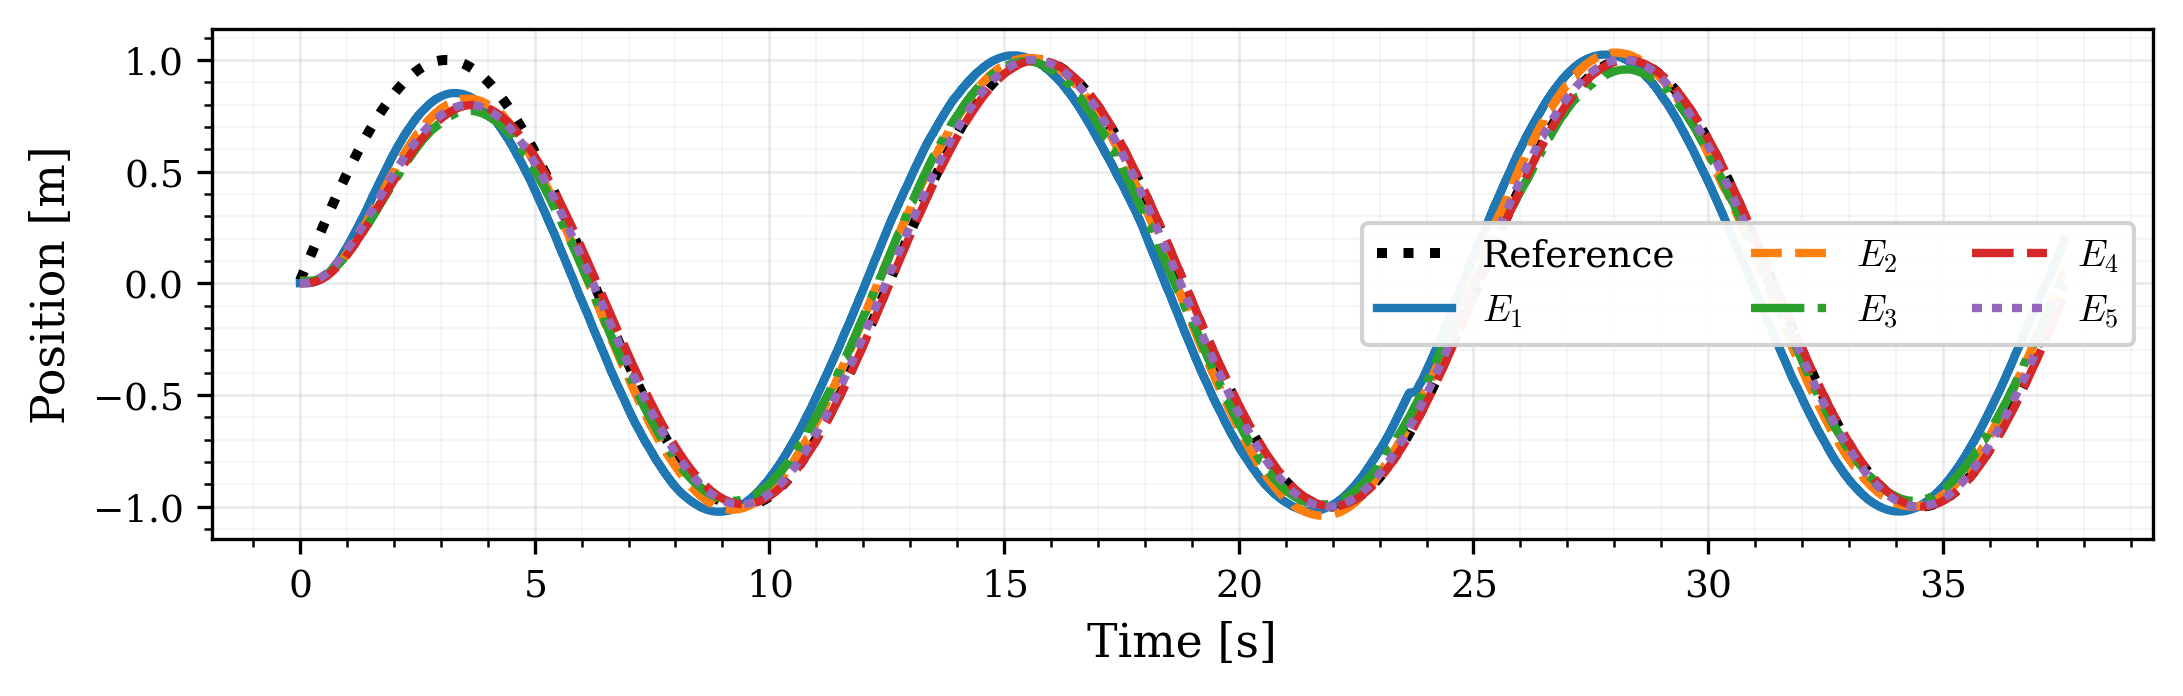
\includegraphics[width=\linewidth]{experiment_plots/tracking_x.png}\caption{$x(t)$.}\end{subfigure}
    \\
    \begin{subfigure}{\textwidth}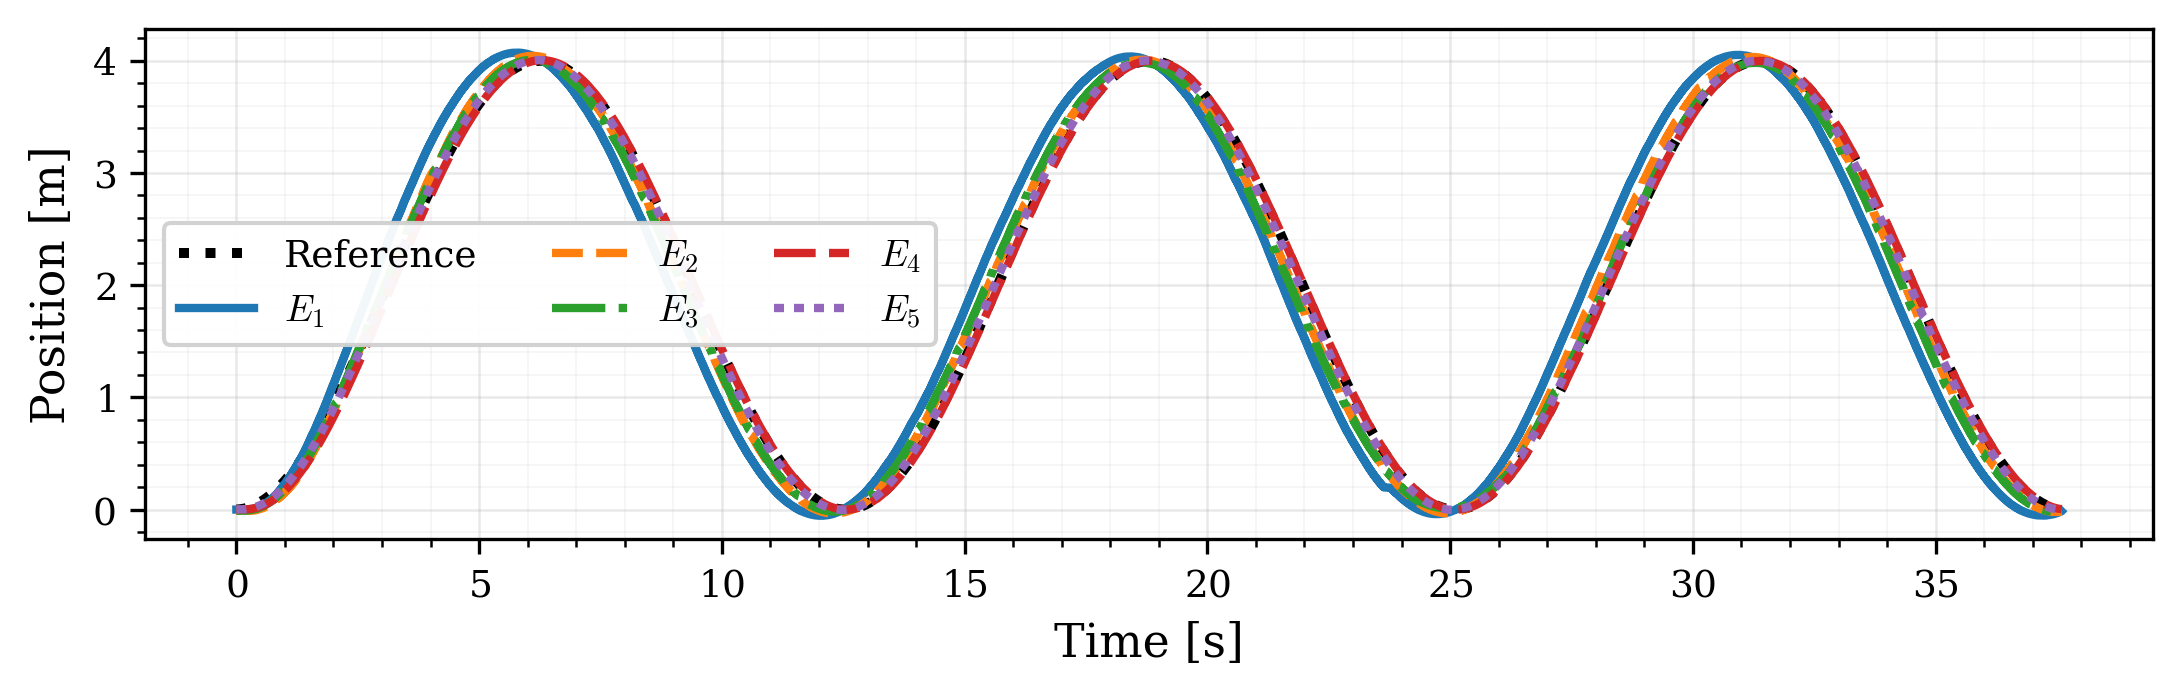
\includegraphics[width=\linewidth]{experiment_plots/tracking_y.png}\caption{$y(t)$.}\end{subfigure}
    \\
    \begin{subfigure}{\textwidth}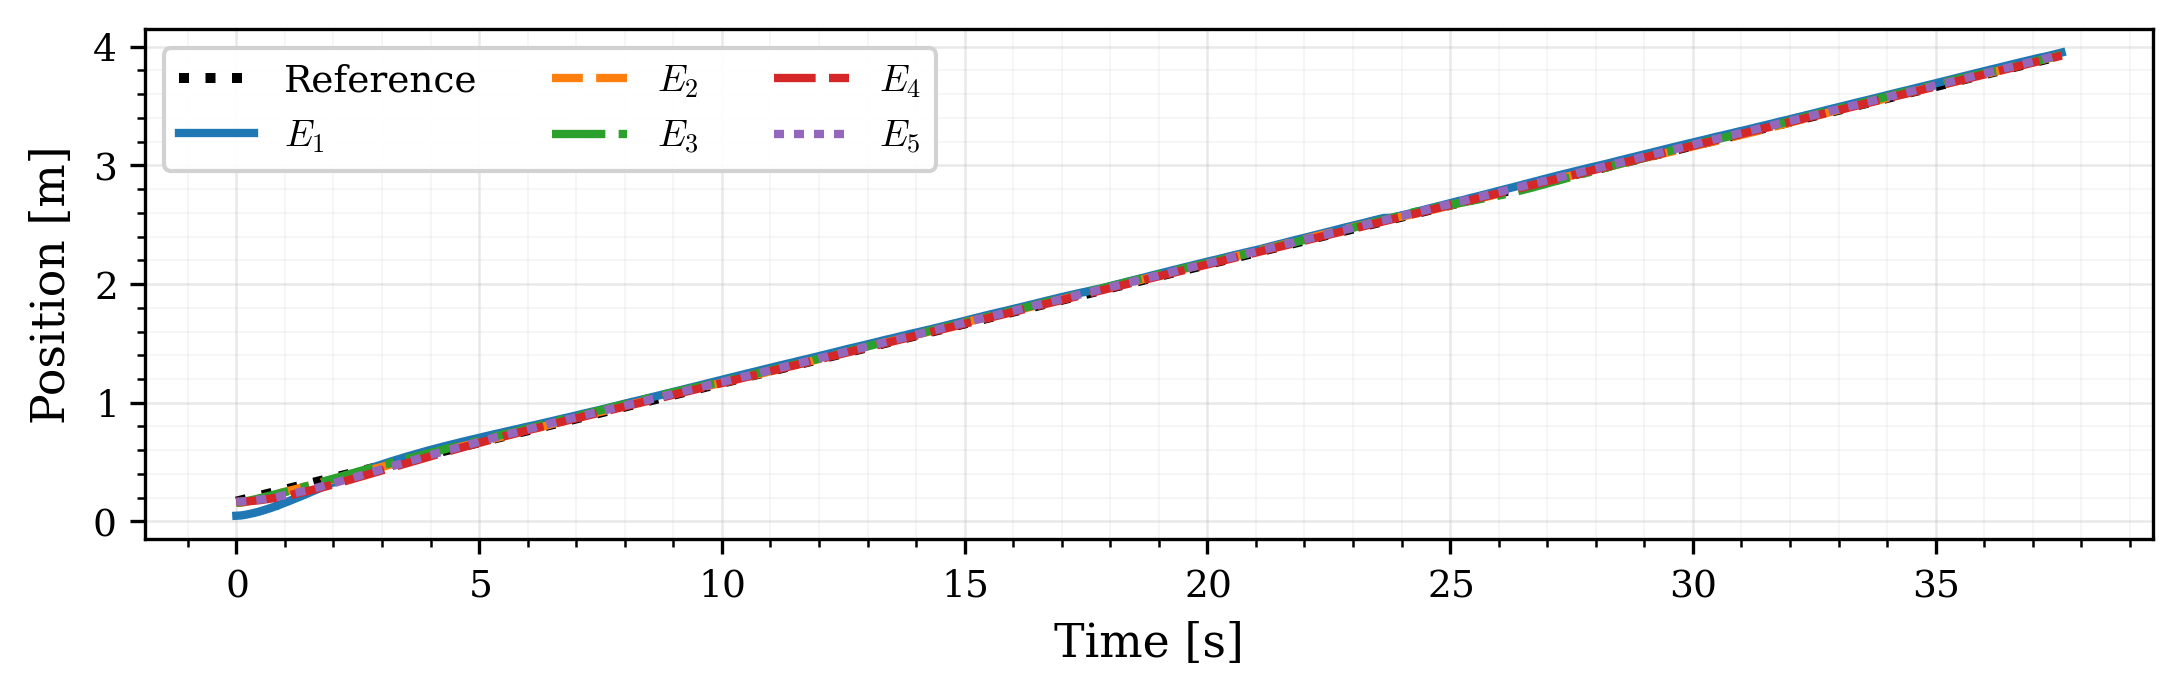
\includegraphics[width=\linewidth]{experiment_plots/tracking_z.png}\caption{$z(t)$.}\end{subfigure}
    \caption{Per-axis position tracking against the reference (dashed).}
    \label{fig:overlay-tracking-xyz}
\end{figure}

In the per-axis tracking plots, E1 (blue) lags the reference visibly in both $x$ and $y$; E2 and E3 also lag but by a smaller amount; E4 and E5 lie underneath the reference within line width. The $z$-axis is tracked tightly by all five experiments, since it is excited only by the constant climb rate $v_z = 0.1$~m/s.

\subsubsection{Position and Velocity Errors}

\begin{figure}[H]
    \centering
    \begin{subfigure}{\textwidth}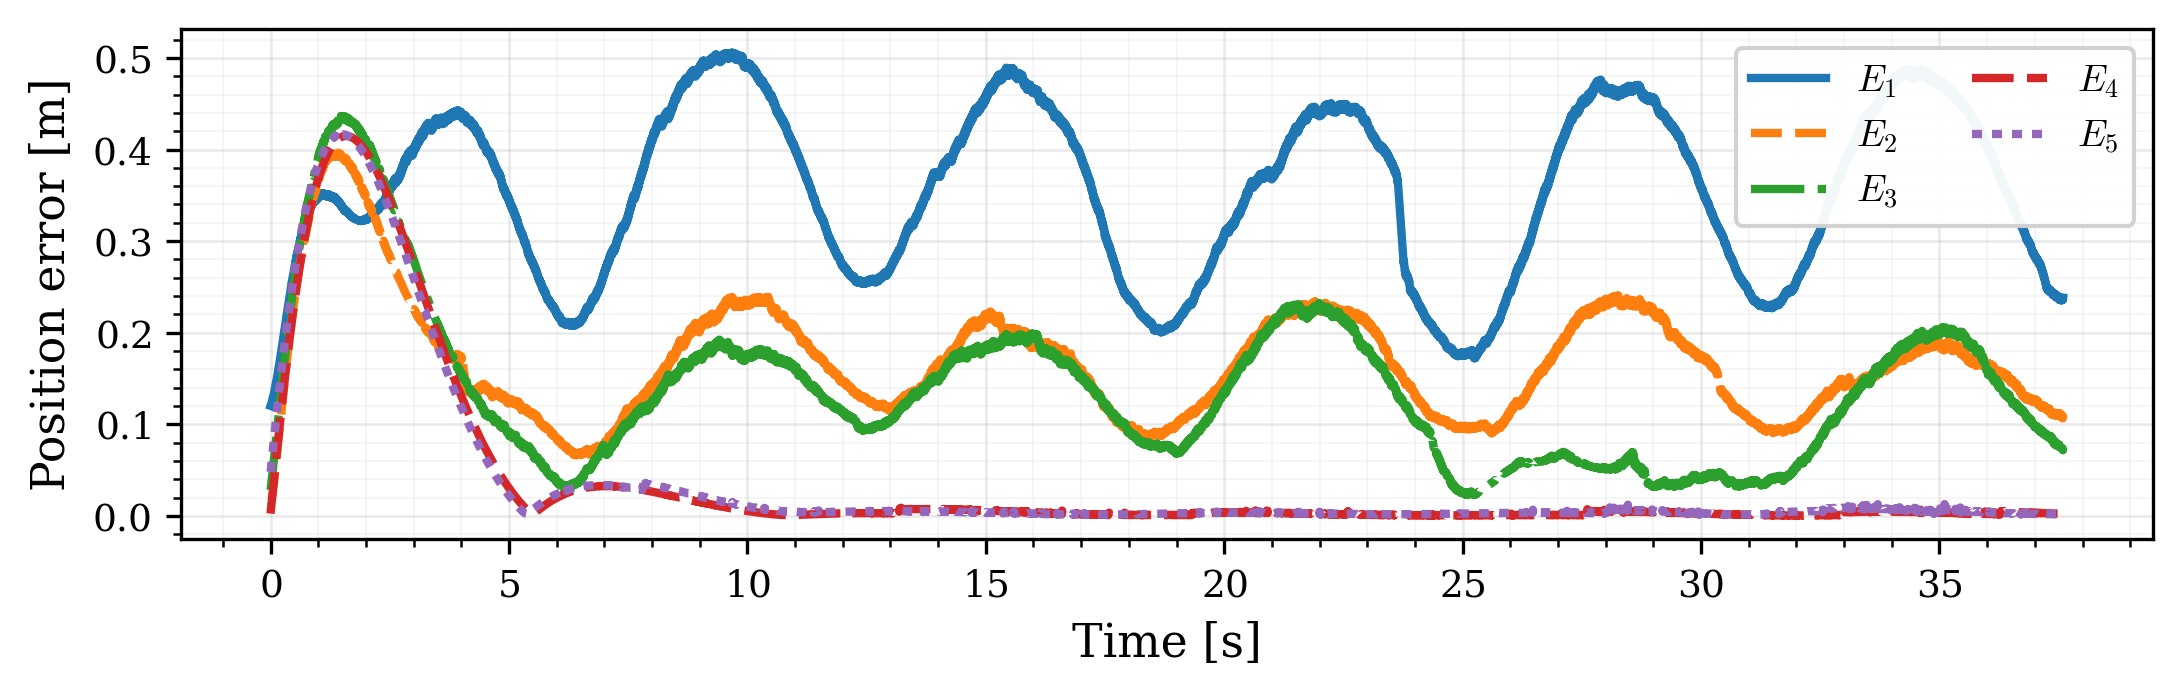
\includegraphics[width=\linewidth]{experiment_plots/error_position.png}\caption{Position-error norm $\|e_x(t)\|$.}\end{subfigure}
    \\
    \begin{subfigure}{\textwidth}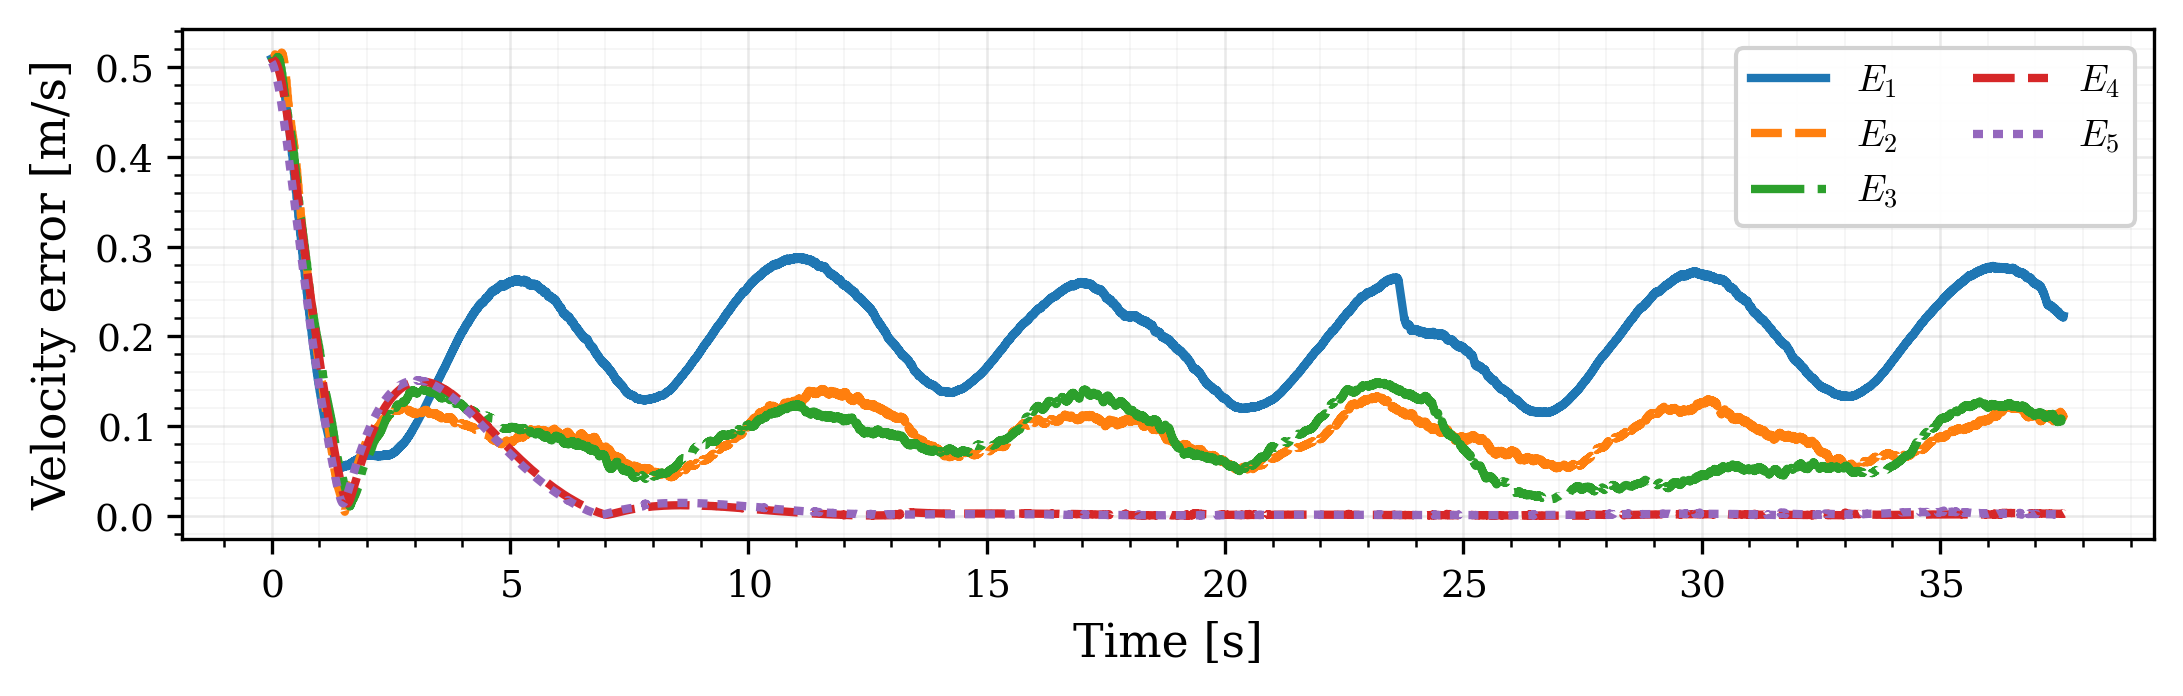
\includegraphics[width=\linewidth]{experiment_plots/error_velocity.png}\caption{Velocity-error norm $\|e_v(t)\|$.}\end{subfigure}
    \caption{Translational tracking errors. The early peak corresponds to the initial transient from the resting pose; afterwards each curve traces the steady-state tracking error of its experiment.}
    \label{fig:overlay-translational-errors}
\end{figure}

The position-error norm separates the experiments cleanly into three bands. E1 oscillates between $0.2$ and $0.5$~m for the entire duration. E2 and E3 are essentially indistinguishable, oscillating between roughly $0.10$ and $0.25$~m. E4 and E5 sit close to zero with a slight rise toward the end of the trajectory but remain below $0.15$~m throughout. The velocity-error norm shows the same banded structure, scaled by the trajectory's characteristic frequency.

\begin{figure}[H]
    \centering
    \begin{subfigure}{\textwidth}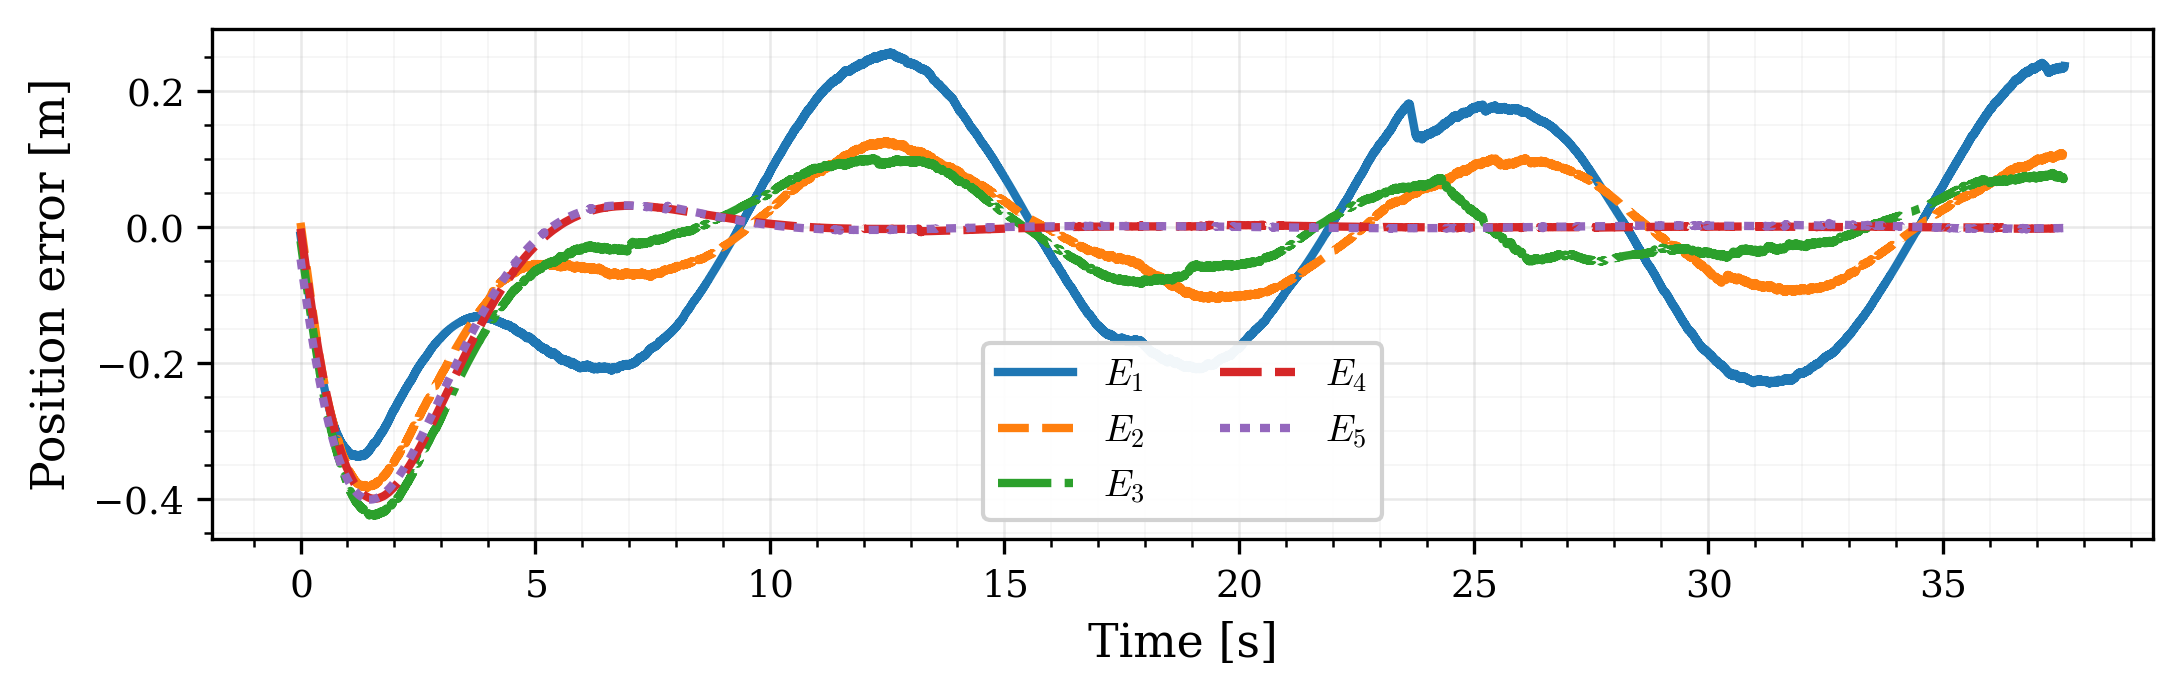
\includegraphics[width=\linewidth]{experiment_plots/error_x.png}\caption{$e_{x,1}(t)$.}\end{subfigure}
    \\
    \begin{subfigure}{\textwidth}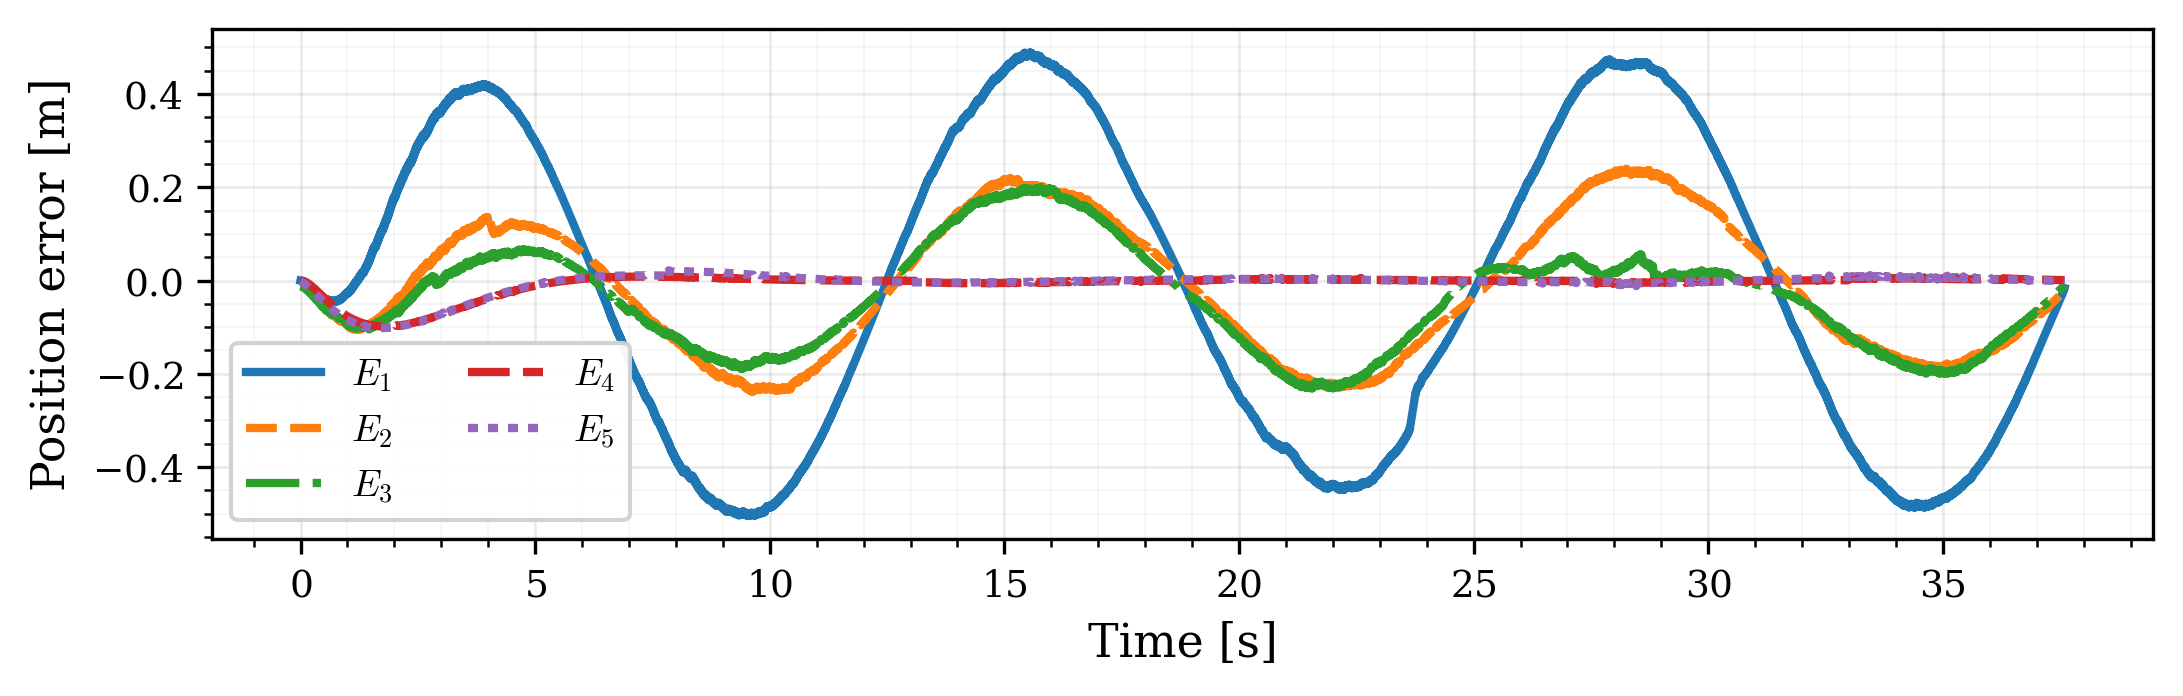
\includegraphics[width=\linewidth]{experiment_plots/error_y.png}\caption{$e_{x,2}(t)$.}\end{subfigure}
    \\
    \begin{subfigure}{\textwidth}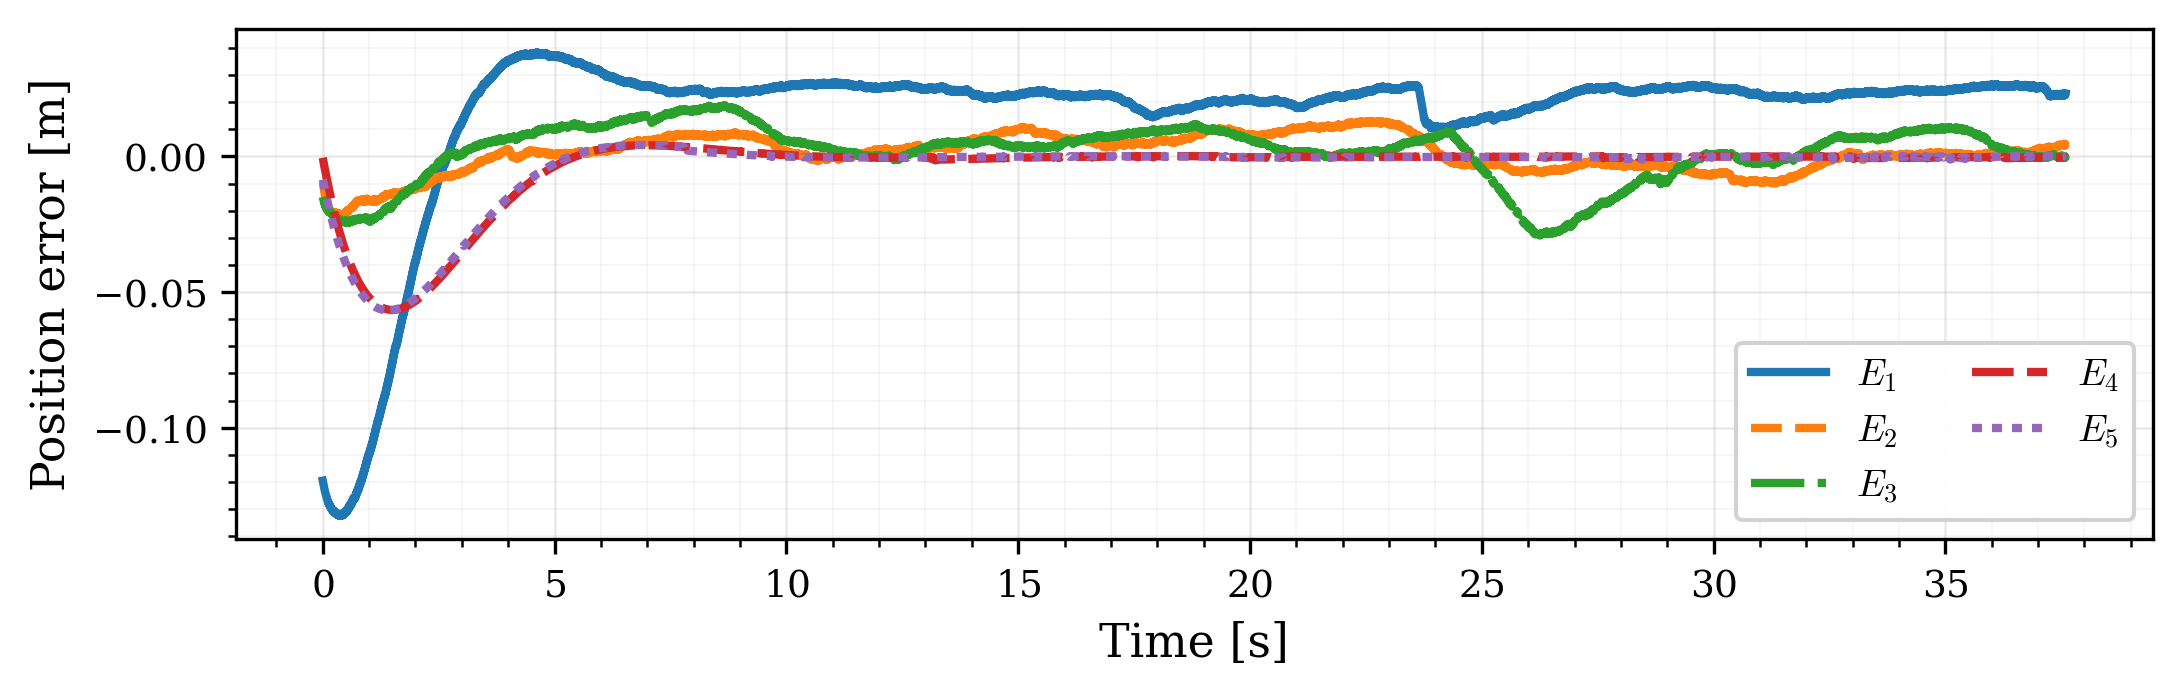
\includegraphics[width=\linewidth]{experiment_plots/error_z.png}\caption{$e_{x,3}(t)$.}\end{subfigure}
    \caption{Position-error components per inertial axis.}
    \label{fig:overlay-ex-axes}
\end{figure}

Decomposing the position error per axis shows that the bulk of E1's error lives in the lateral channels $x$ and $y$, where its components swing between roughly $\pm 0.25$~m and $\pm 0.5$~m respectively. The vertical-axis error $e_{x,3}$ is small and similar across all five experiments (a few centimetres), confirming that the gravity-compensation term in the controller is doing its job in every configuration.

\subsubsection{Attitude Tracking and Errors}

\begin{figure}[H]
    \centering
    \begin{subfigure}{\textwidth}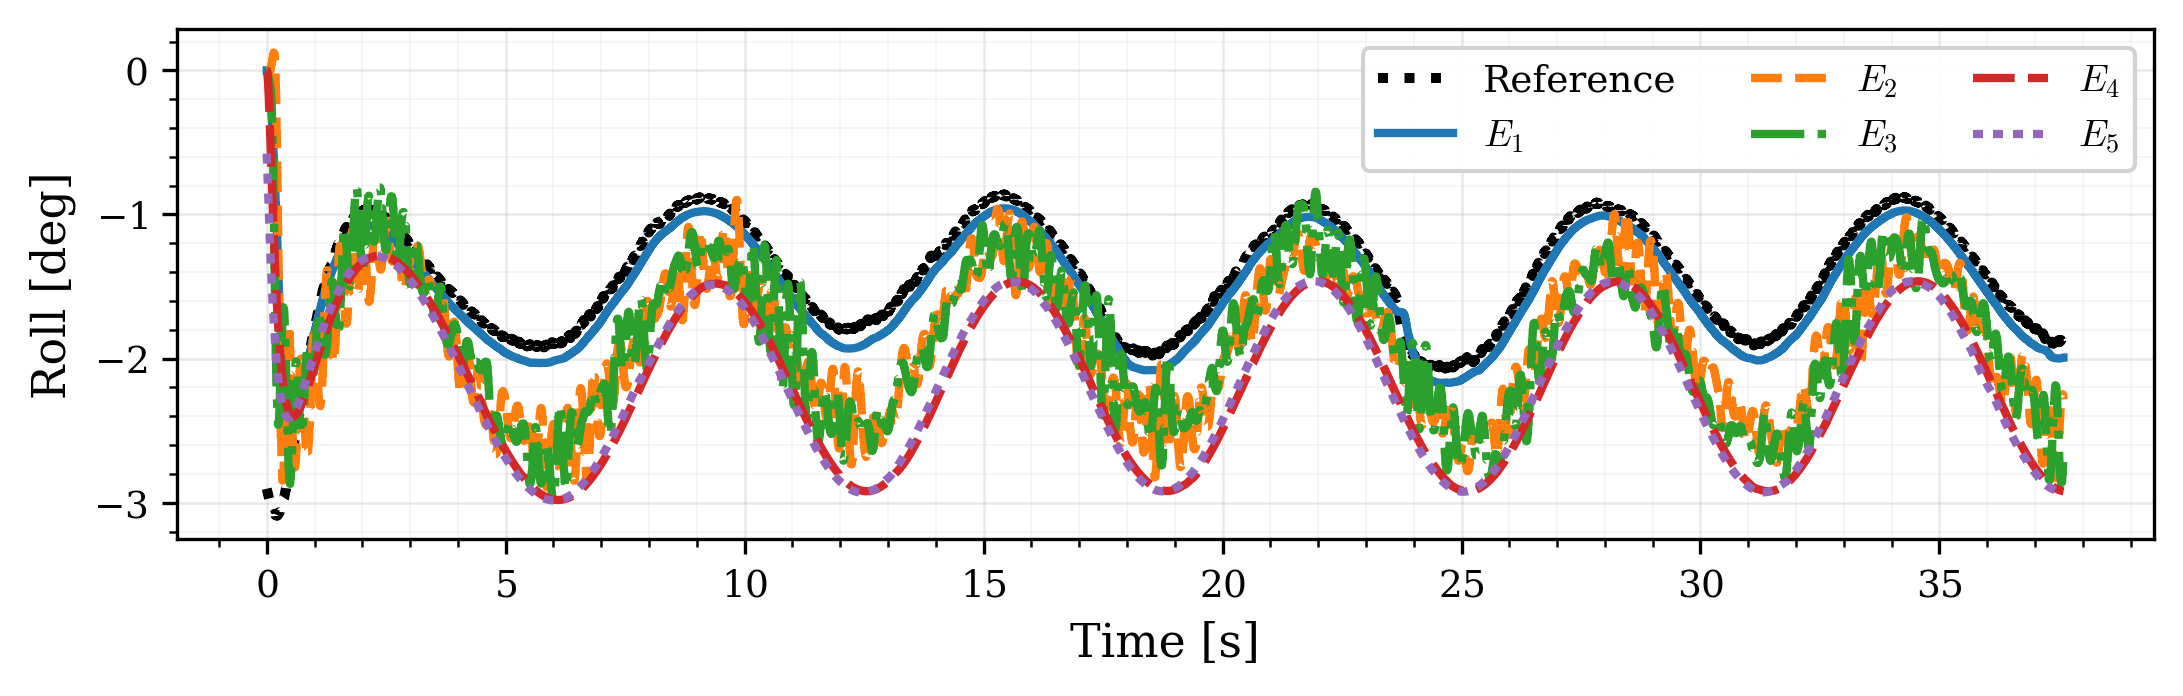
\includegraphics[width=\linewidth]{experiment_plots/tracking_attitude_roll.png}\caption{Roll.}\end{subfigure}
    \\
    \begin{subfigure}{\textwidth}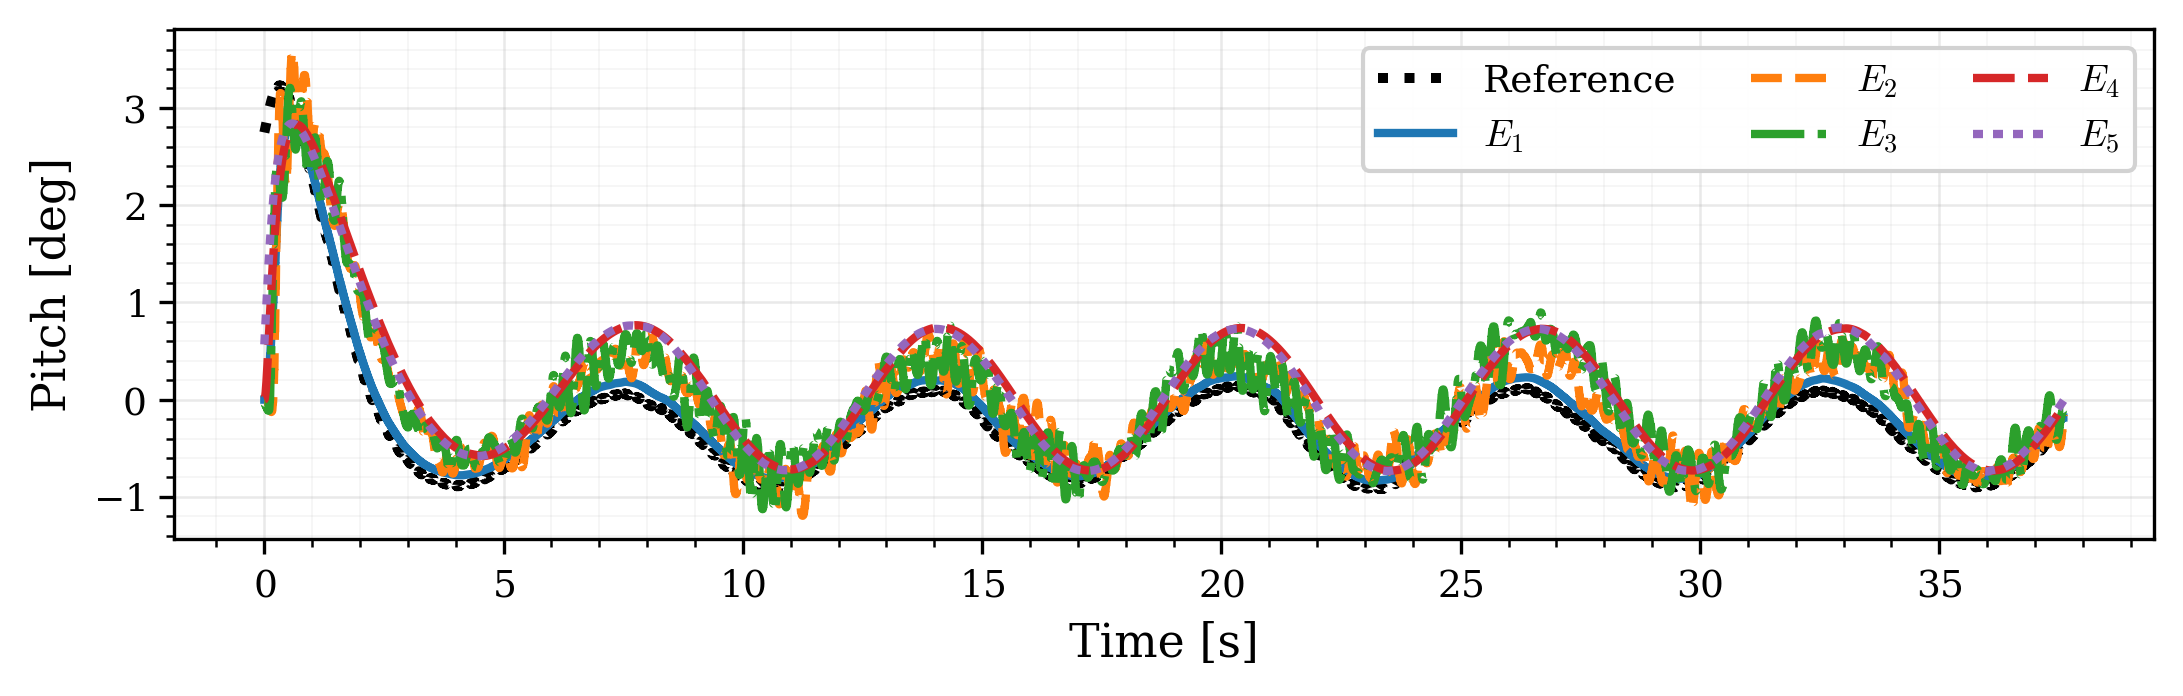
\includegraphics[width=\linewidth]{experiment_plots/tracking_attitude_pitch.png}\caption{Pitch.}\end{subfigure}
    \\
    \begin{subfigure}{\textwidth}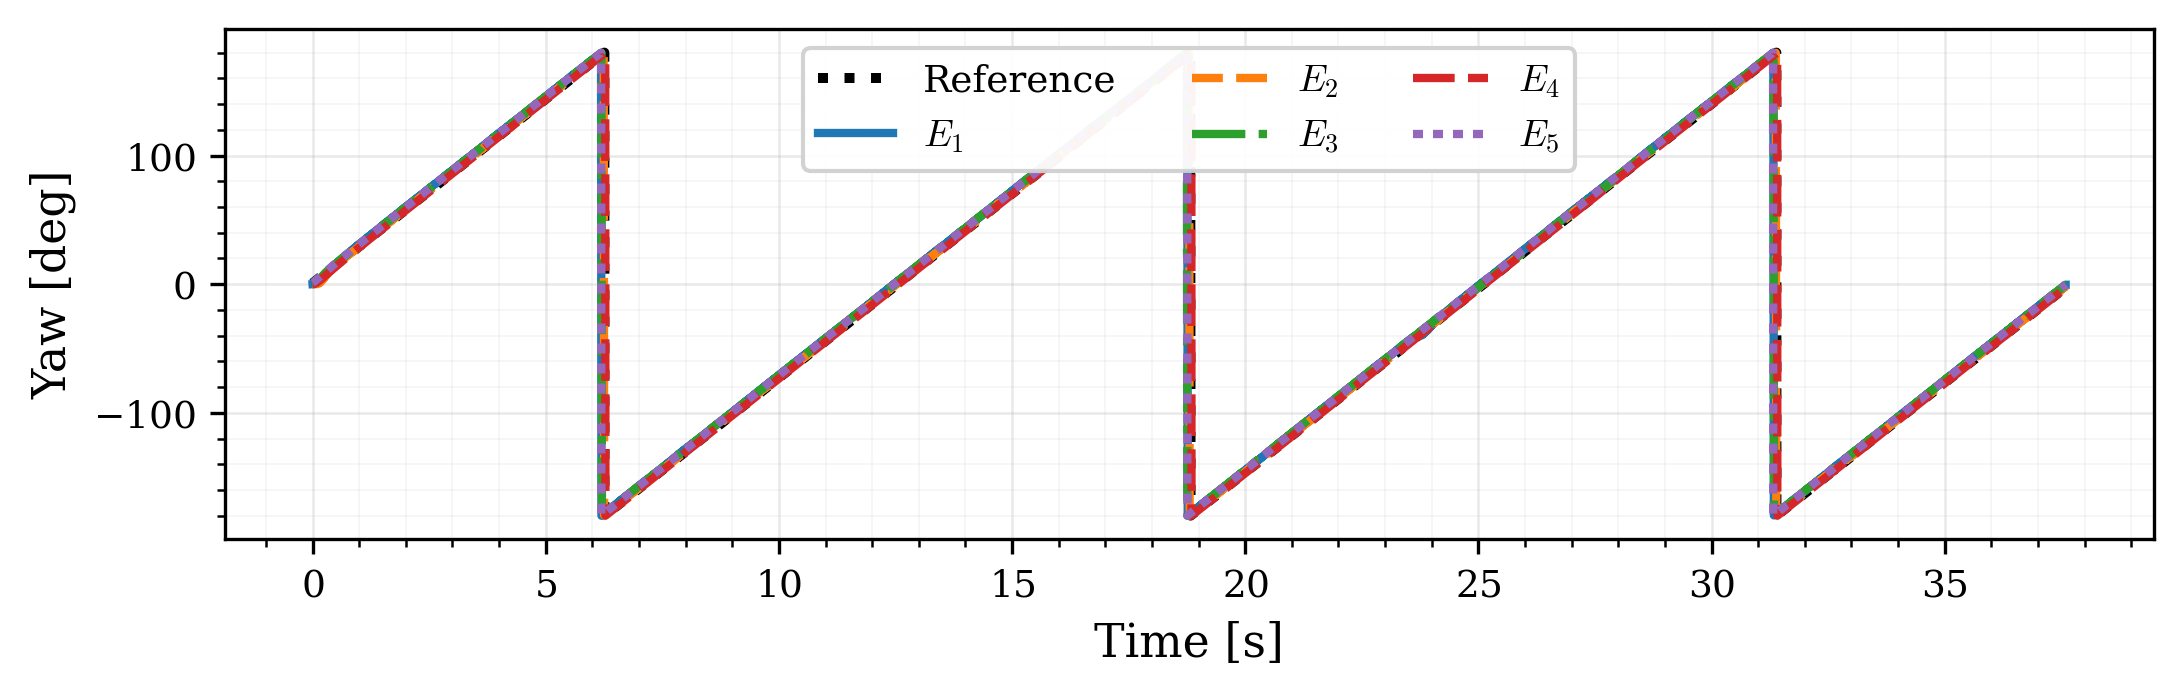
\includegraphics[width=\linewidth]{experiment_plots/tracking_attitude_yaw.png}\caption{Yaw.}\end{subfigure}
    \caption{Attitude tracking in roll/pitch/yaw against the reference signal extracted from the trajectory generator.}
    \label{fig:overlay-attitude-rpy}
\end{figure}

In the attitude plots, all five experiments follow the small-amplitude roll/pitch oscillations demanded by the helix manoeuvre, with E1 most clearly offset from the reference and E4/E5 essentially overlaying it. The yaw channel is a sawtooth that ramps from $-180^\circ$ to $+180^\circ$ once per revolution; all five experiments track it indistinguishably.

\begin{figure}[H]
    \centering
    \begin{subfigure}{\textwidth}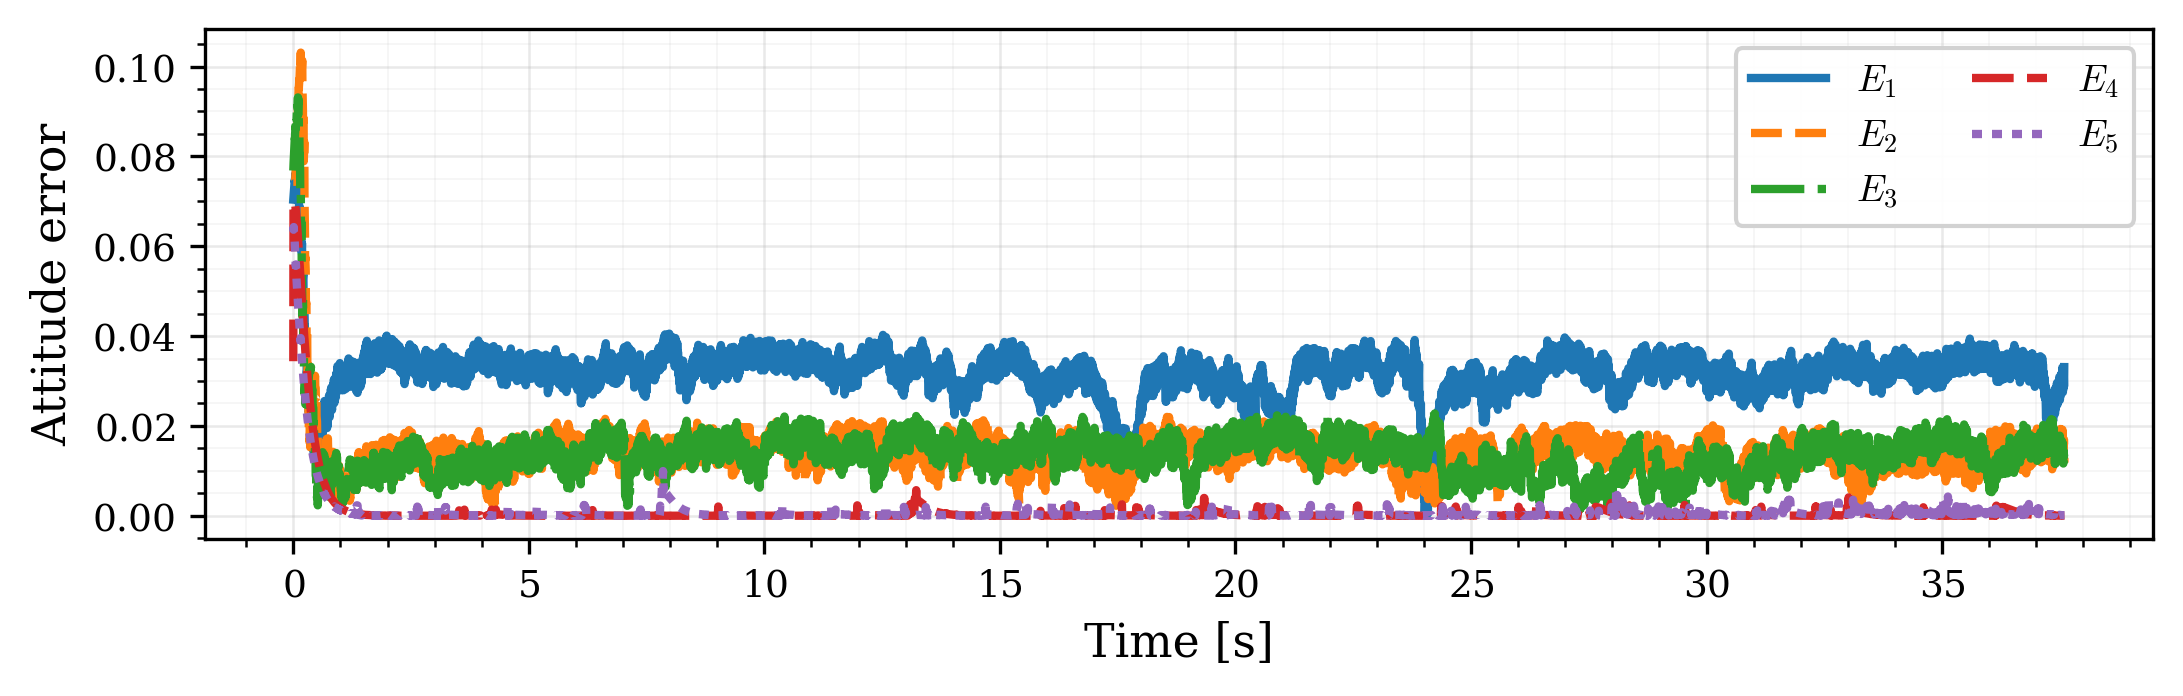
\includegraphics[width=\linewidth]{experiment_plots/error_attitude.png}\caption{Attitude-error norm $\|e_R(t)\|$.}\end{subfigure}
    \\
    \begin{subfigure}{\textwidth}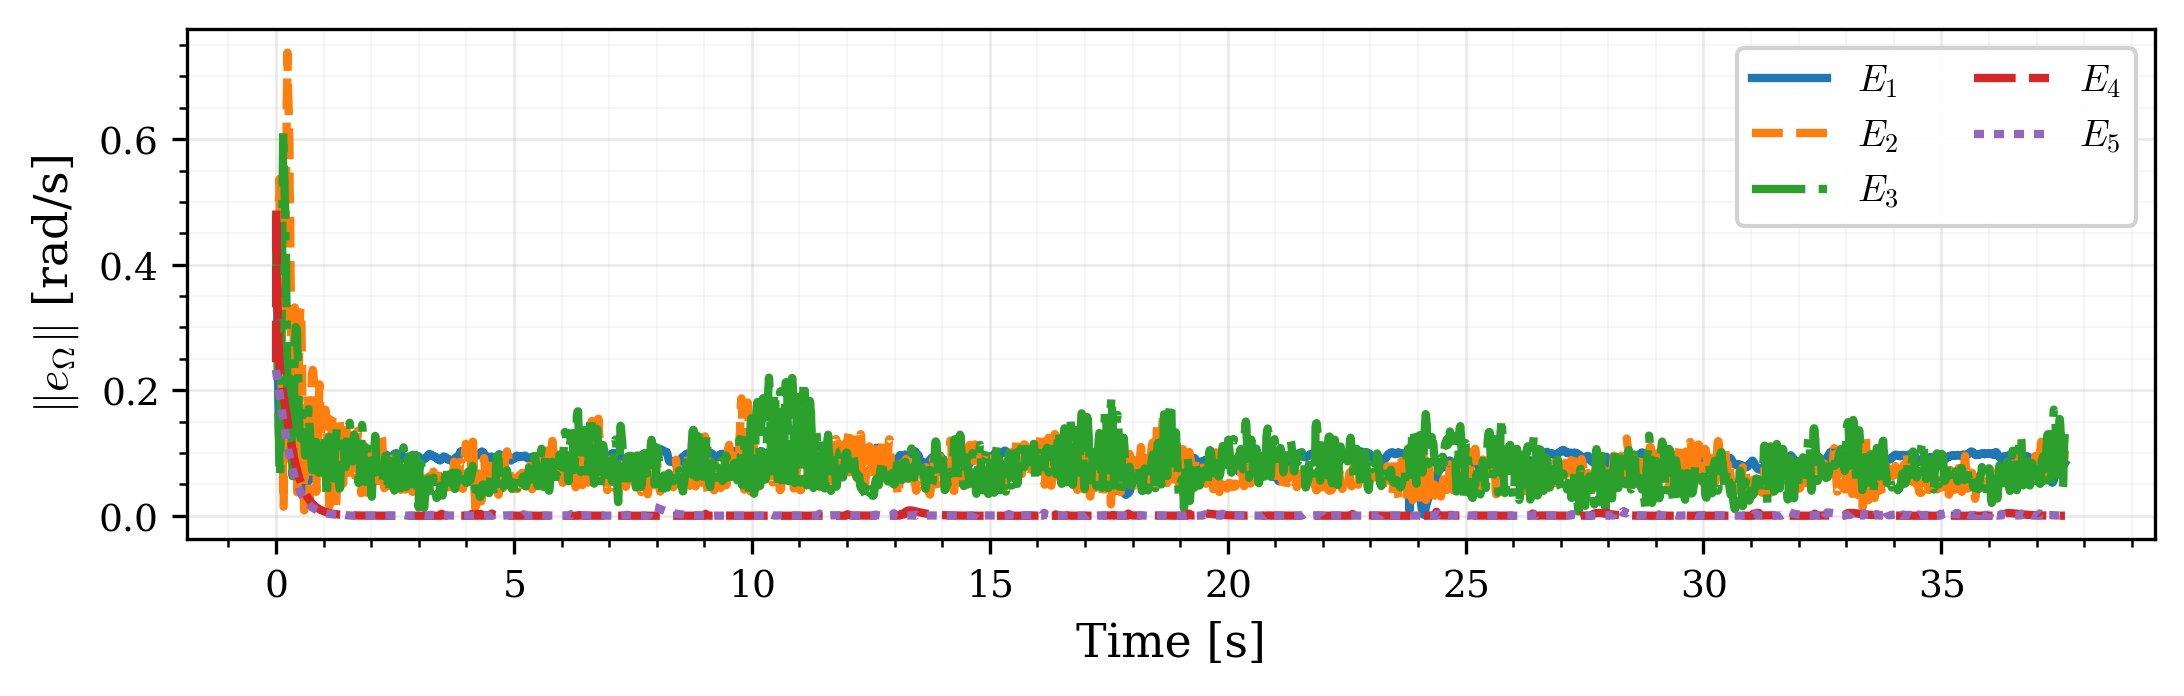
\includegraphics[width=\linewidth]{experiment_plots/error_angular_velocity.png}\caption{Angular-velocity-error norm $\|e_\Omega(t)\|$.}\end{subfigure}
    \caption{Rotational tracking errors.}
    \label{fig:overlay-rotational-errors}
\end{figure}

The rotational error plots show the same banded structure as the translational ones: E1 settles around $\|e_R\| \approx 0.03$, E2 and E3 around $\|e_R\| \approx 0.015$, and E4 and E5 sit at essentially zero with only a brief spike near $t \approx 30$~s. The angular-velocity-error norm $\|e_\Omega\|$ is dominated by an initial transient of amplitude $\approx 0.7$~rad/s for all five experiments and then settles into the same banded structure thereafter.

\subsubsection{Control Outputs}

\begin{figure}[!htbp]
    \centering
    \begin{subfigure}{0.92\textwidth}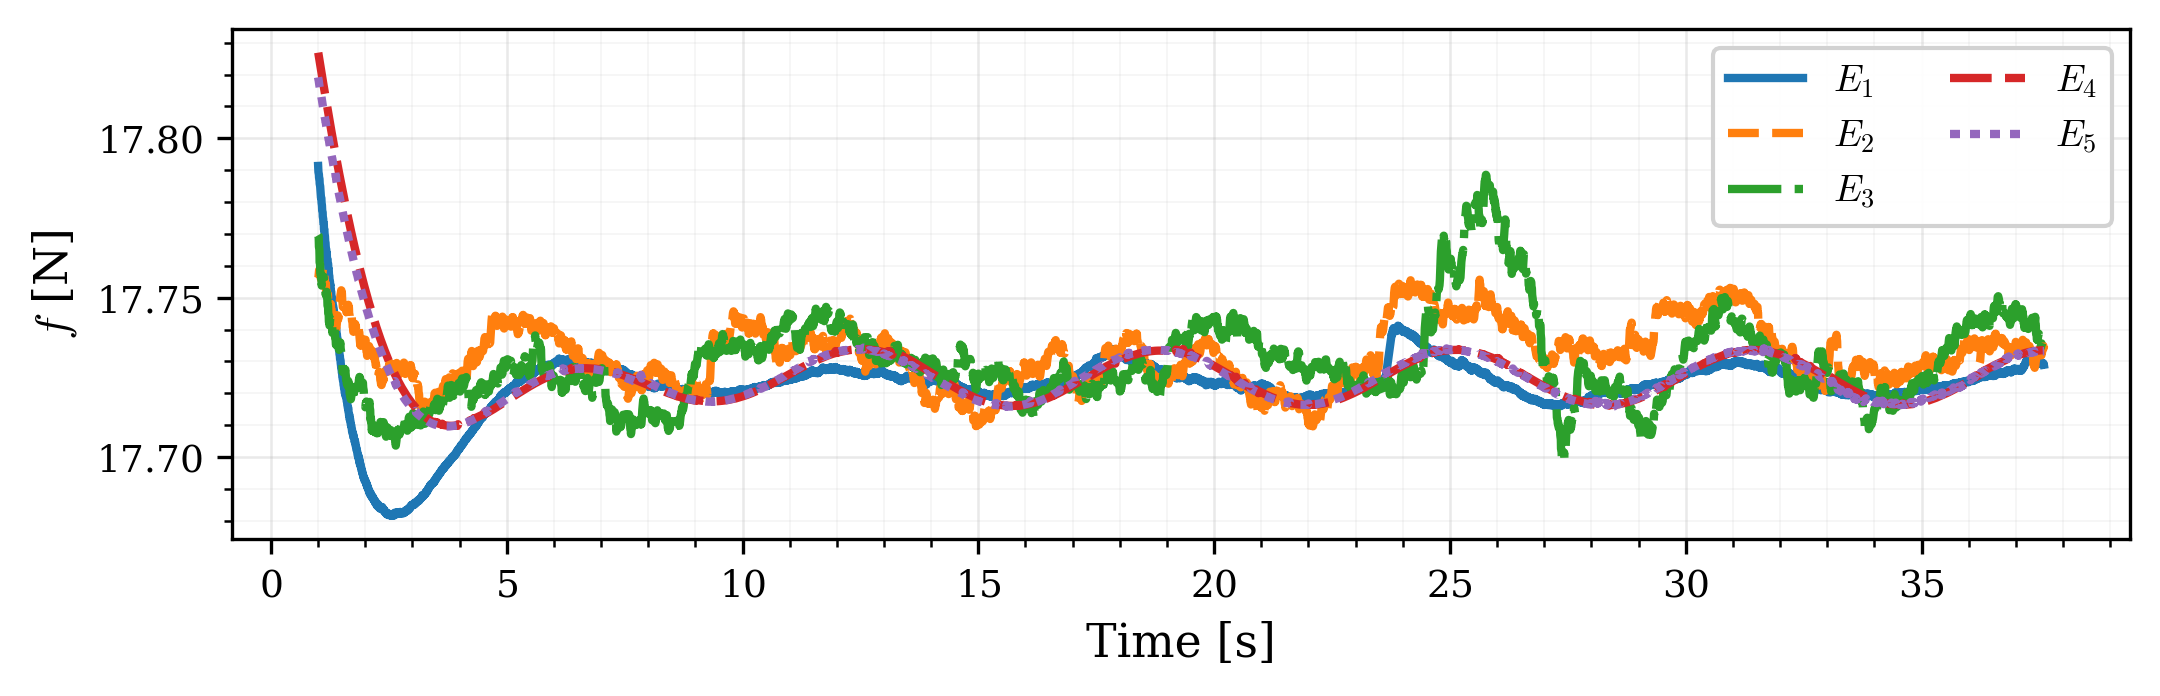
\includegraphics[width=\linewidth]{experiment_plots/control_f.png}\caption{Total thrust $f(t)$.}\end{subfigure}
    \\
    \begin{subfigure}{0.92\textwidth}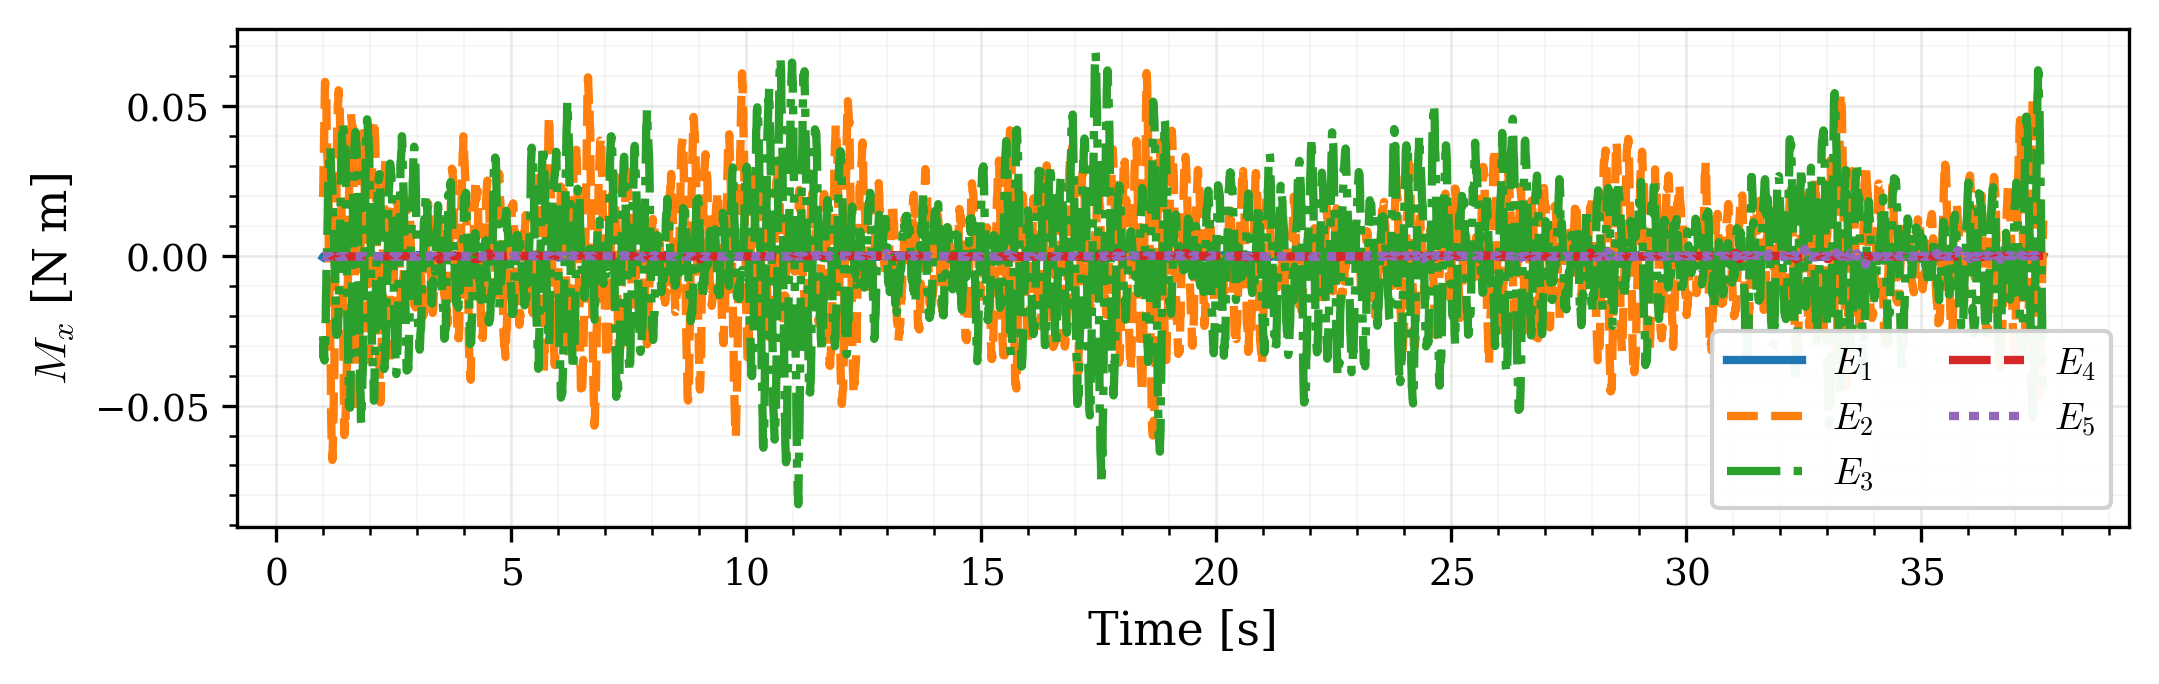
\includegraphics[width=\linewidth]{experiment_plots/control_Mx.png}\caption{Roll moment $M_x(t)$.}\end{subfigure}
    \\
    \begin{subfigure}{0.92\textwidth}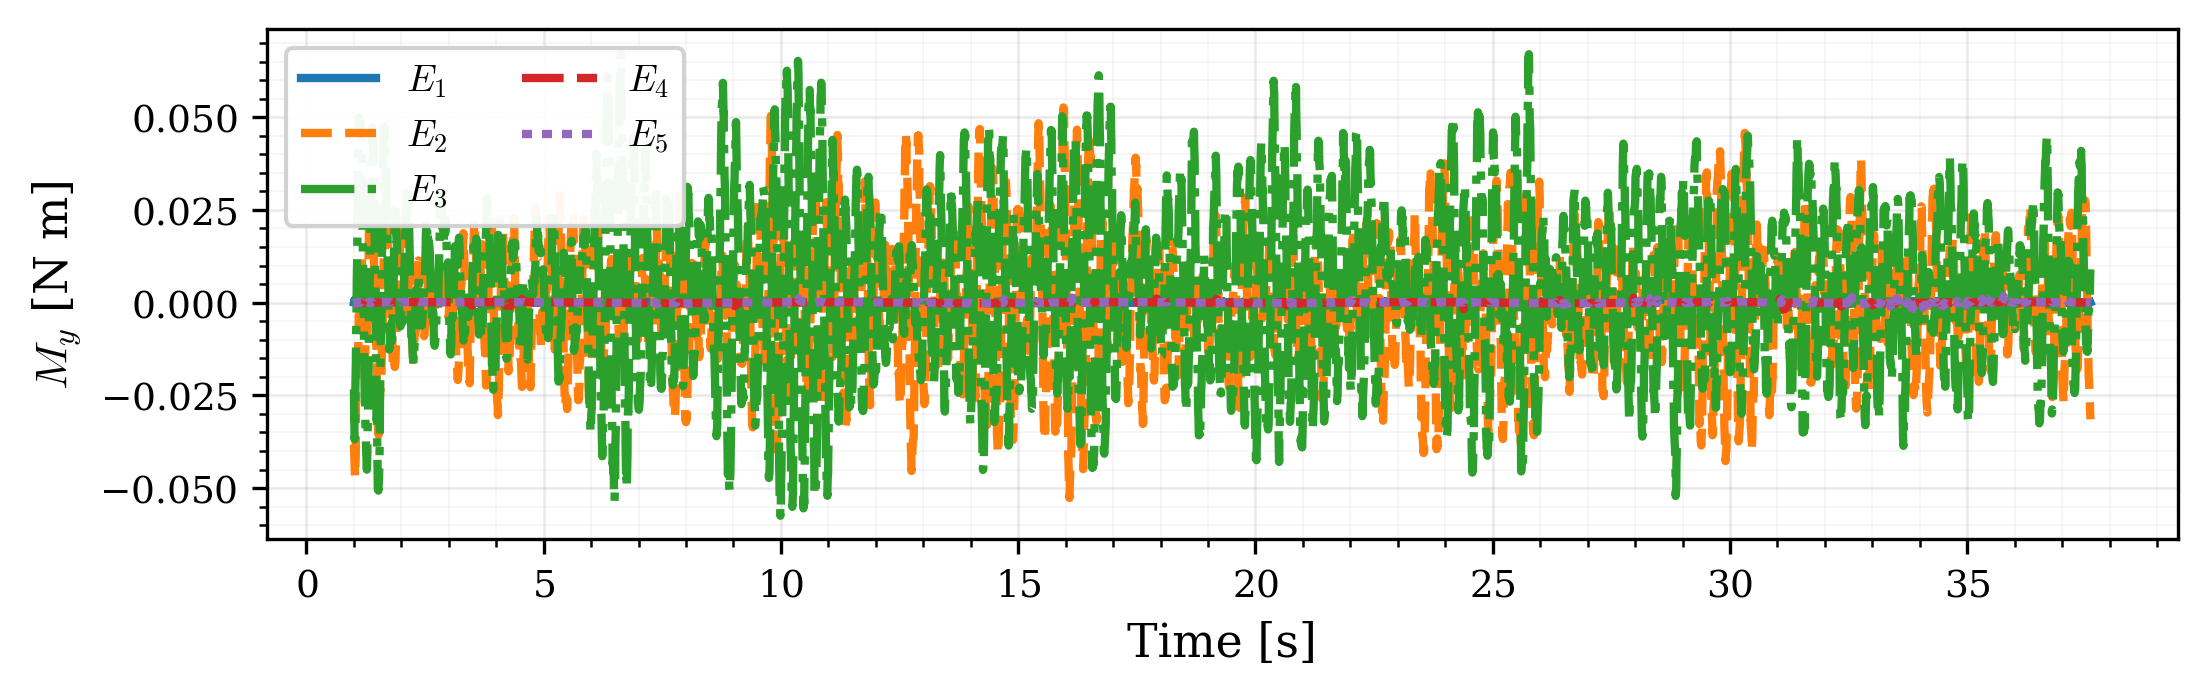
\includegraphics[width=\linewidth]{experiment_plots/control_My.png}\caption{Pitch moment $M_y(t)$.}\end{subfigure}
    \\
    \begin{subfigure}{0.92\textwidth}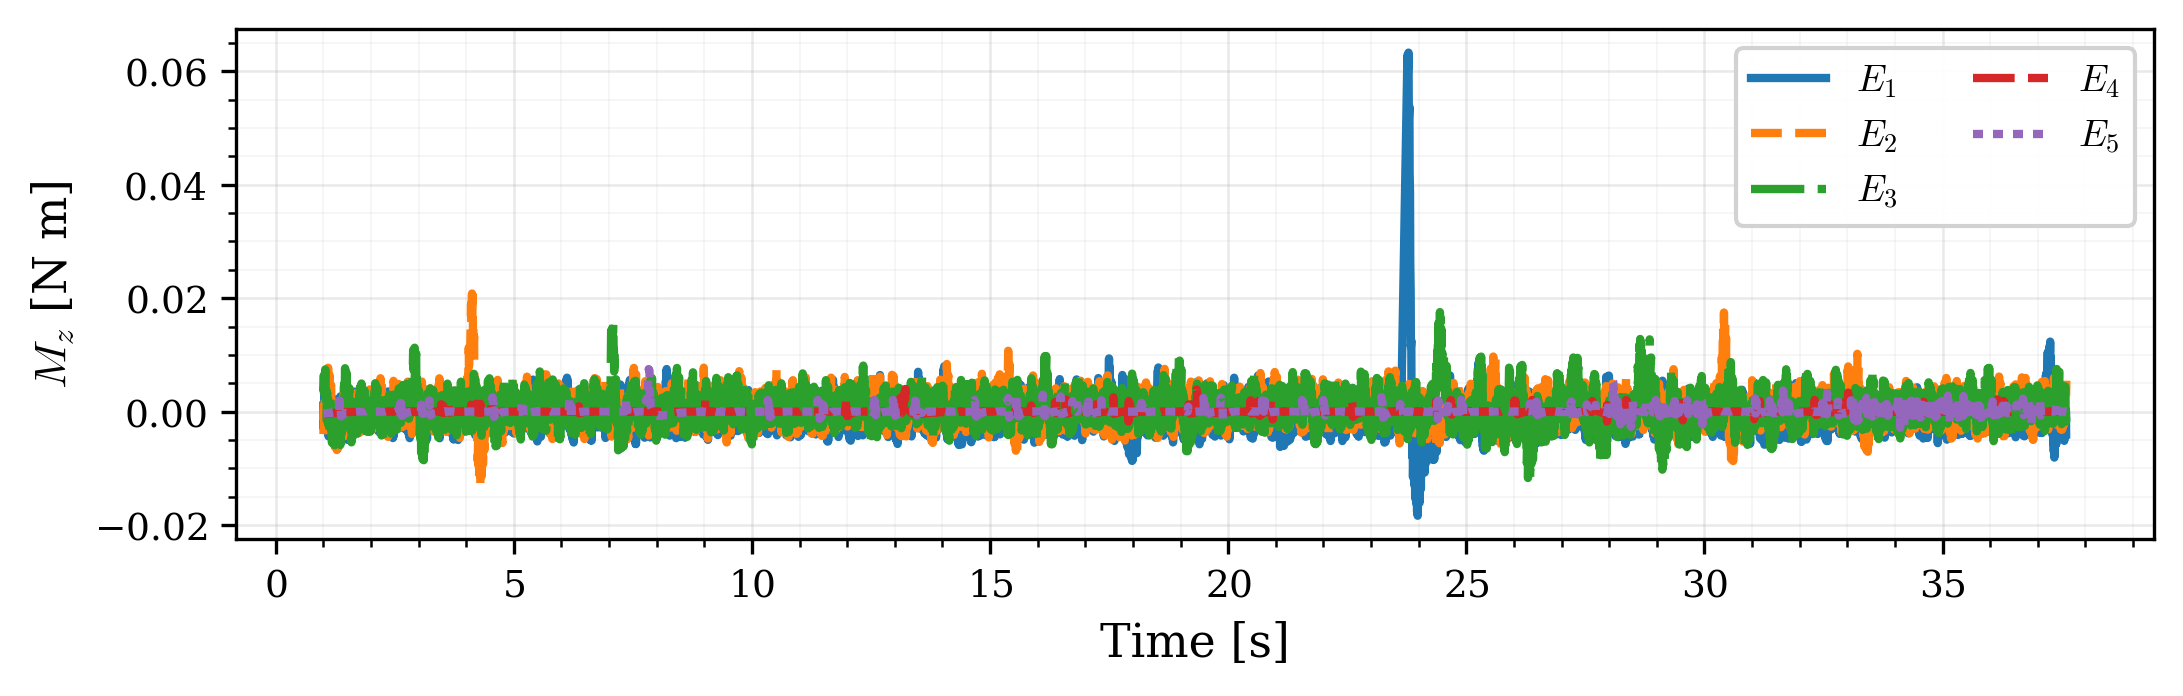
\includegraphics[width=\linewidth]{experiment_plots/control_Mz.png}\caption{Yaw moment $M_z(t)$.}\end{subfigure}
    \caption{Commanded total thrust and body-frame moments, plotted from $t = 1$~s to mask the controller's initial transient that would otherwise compress the steady-state vertical scale.}
    \label{fig:overlay-control-fM}
\end{figure}

The total thrust $f$ tracks the vehicle weight $mg \approx 17.7$~N closely in every experiment, with small ripples that follow the trajectory's vertical acceleration. The body-frame moments tell a sharper story: the roll and pitch moments $M_x, M_y$ commanded by the controller are markedly noisier in E1, E2, E3 (PhysX configurations) than in E4, E5 (custom solver), where they sit near zero with very little chatter. This is consistent with PhysX's solver introducing high-frequency joint-constraint and discretisation effects that the controller continually compensates for, whereas the custom solver presents a perfectly clean rigid-body system whose ideal feed-forward exactly cancels the dynamics. The yaw-moment trace shows a brief spike near $t \approx 23$~s in E1, coinciding with the yaw-wraparound discontinuity in the reference at the end of one revolution.

\begin{figure}[H]
    \centering
    \begin{subfigure}{0.49\textwidth}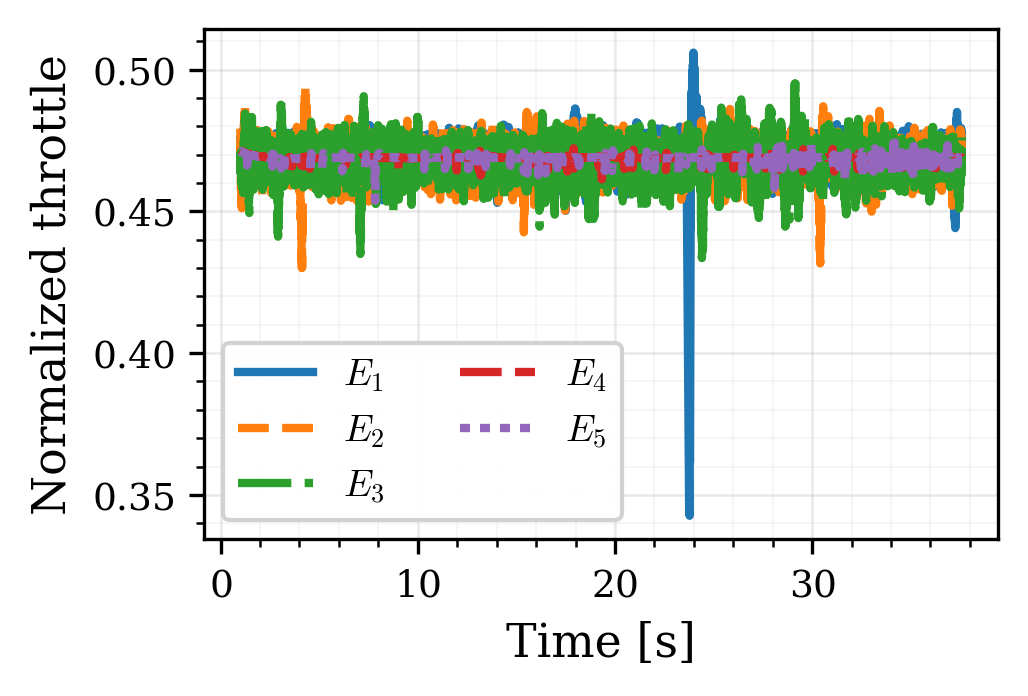
\includegraphics[width=\linewidth]{experiment_plots/control_throttle_rotor1.png}\caption{Rotor 0.}\end{subfigure}
    \hfill
    \begin{subfigure}{0.49\textwidth}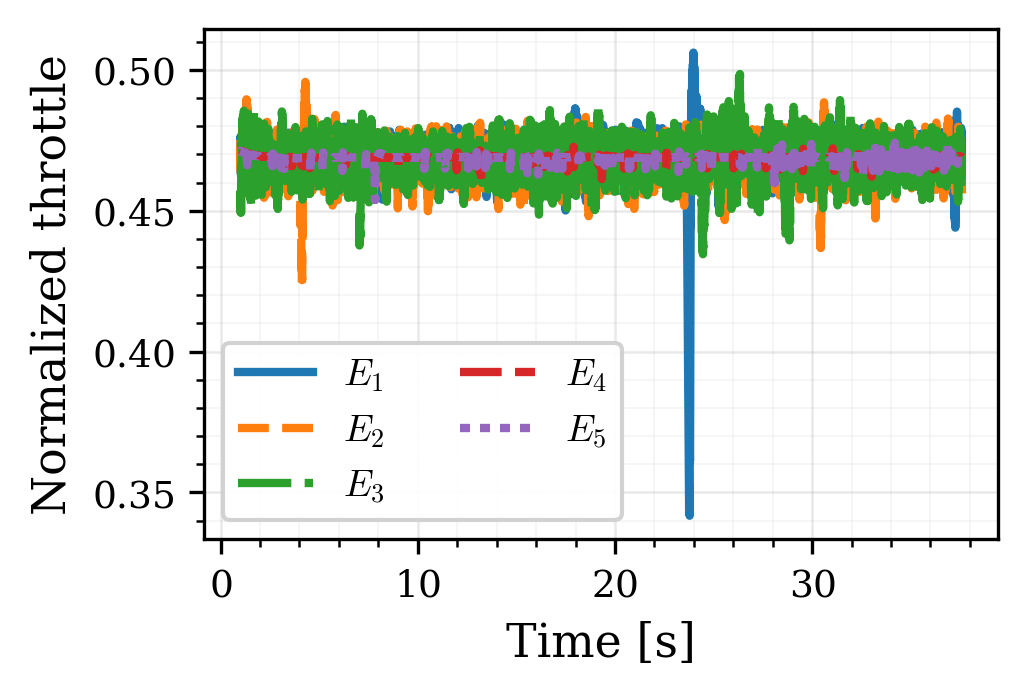
\includegraphics[width=\linewidth]{experiment_plots/control_throttle_rotor2.png}\caption{Rotor 1.}\end{subfigure}
    \\[0.4em]
    \begin{subfigure}{0.49\textwidth}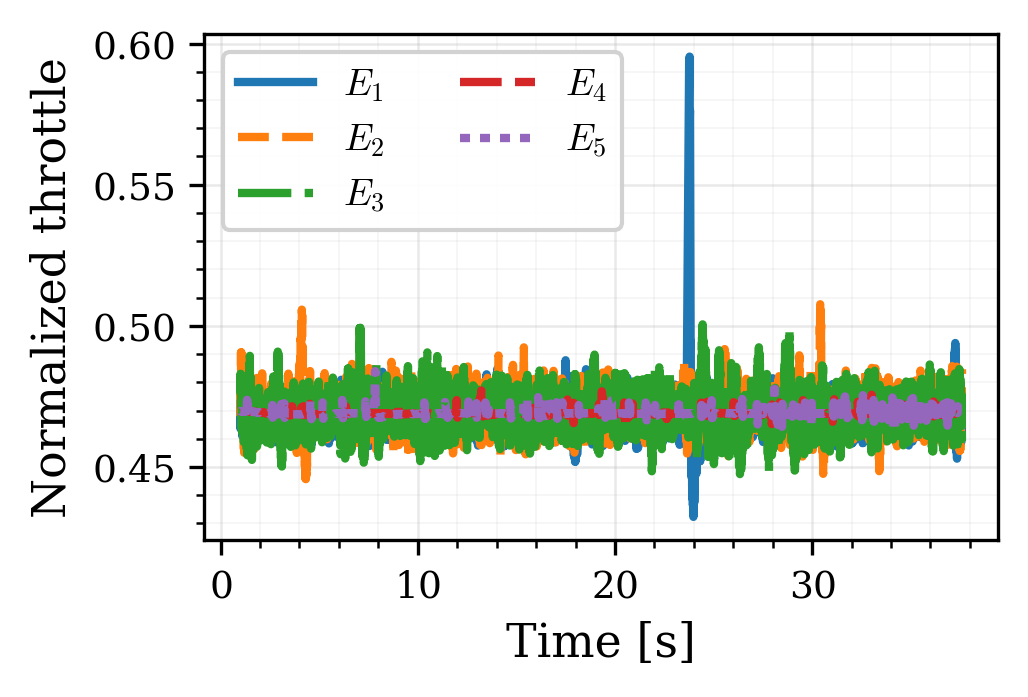
\includegraphics[width=\linewidth]{experiment_plots/control_throttle_rotor3.png}\caption{Rotor 2.}\end{subfigure}
    \hfill
    \begin{subfigure}{0.49\textwidth}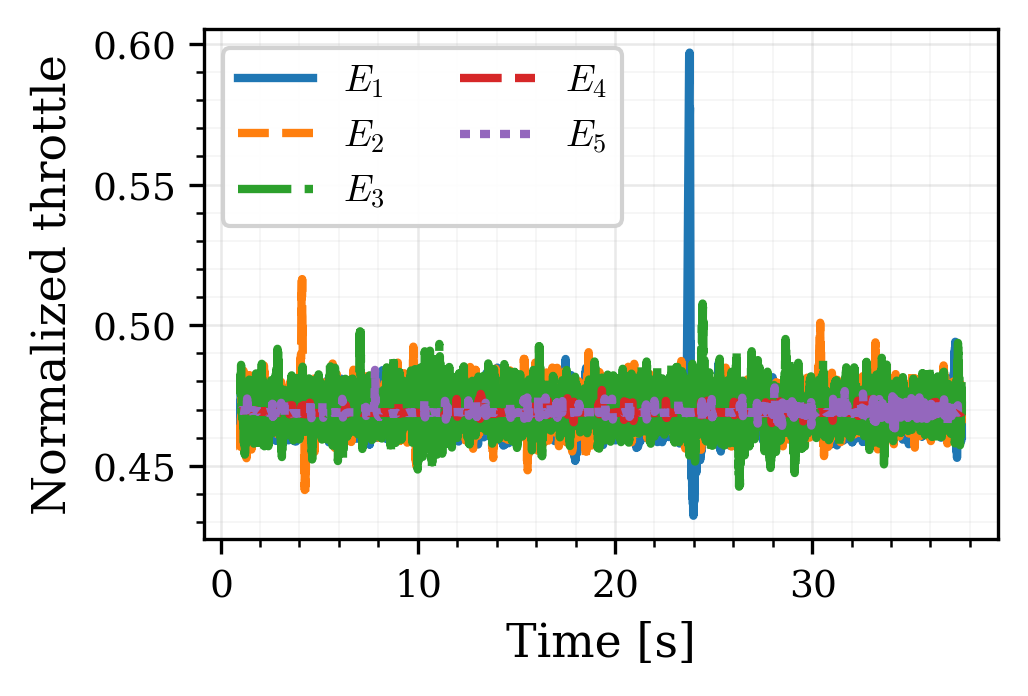
\includegraphics[width=\linewidth]{experiment_plots/control_throttle_rotor4.png}\caption{Rotor 3.}\end{subfigure}
    \caption{Per-rotor normalised throttle commands $u_0, u_1, u_2, u_3$ for all five configurations. All four channels stay strictly within the saturation bounds $[0, 1]$ throughout the trajectory in every experiment.}
    \label{fig:overlay-rotors}
\end{figure}

The per-rotor throttles cluster tightly around $0.46$--$0.48$ in steady state, well clear of the $[0, 1]$ saturation bounds. The yaw-wraparound transient at $t \approx 23$~s is visible as a brief spike in two of the rotors (the same event seen in $M_z$).

\subsection{Aggregate Metrics}
\label{sec:cross-experiment}

The aggregate tracking metrics across all five experiments are summarised in Table~\ref{tab:metrics-summary}.

\begin{table}[H]
    \centering
    \caption{Aggregate tracking metrics on the elliptic-helix benchmark, all five configurations. Errors are the controller-internal error variables defined in Section~\ref{sec:metrics}.}
    \label{tab:metrics-summary}
    \footnotesize
    \renewcommand{\arraystretch}{1.2}
    \begin{tabular}{@{}lcccccc@{}}
        \toprule
        Configuration & $\mathrm{RMS}_{e_x}$~[m] & $\max\|e_x\|$~[m] & $\mathrm{RMS}_{e_v}$~[m/s] & $\mathrm{RMS}_{e_R}$~[--] & $\max\|e_R\|$~[--] & $\mathrm{RMS}_{e_\Omega}$~[rad/s] \\
        \midrule
        E1: Ideal block      & $0.367$ & $0.506$ & $0.209$ & $0.0327$ & $0.0405$ & $0.0912$ \\
        E2: F450 lumped      & $0.180$ & $0.241$ & $0.112$ & $0.0164$ & $0.0220$ & $0.0879$ \\
        E3: F450 distributed & $0.163$ & $0.232$ & $0.110$ & $0.0155$ & $0.0235$ & $0.0911$ \\
        E4: Custom RK4       & $0.102$ & $0.033$ & $0.0735$ & $0.00518$ & $0.00570$ & $0.0219$ \\
        E5: Custom Euler     & $0.102$ & $0.038$ & $0.0695$ & $0.00412$ & $0.00995$ & $0.0155$ \\
        \bottomrule
    \end{tabular}
\end{table}

\subsection{Discussion}
\label{sec:results-discussion}

The plots and the metrics in Table~\ref{tab:metrics-summary} separate the five experiments into three clear bands: E1 alone (high error), E2 and E3 together (intermediate error, indistinguishable from each other), and E4 and E5 together (low error, also indistinguishable from each other). The size of the gap between adjacent bands reveals which modelling choices matter and which do not.

\paragraph{E2 vs.\ E1 (effect of articulation).} Replacing the single rigid block with the F450 articulation reduced the RMS position error from $0.367$~m to $0.180$~m and the RMS attitude error by roughly the same factor. The improvement is consistent across $x$, $y$, $z$, and the rotational channels. A plausible explanation is that the ideal block in E1 carries the F450's \emph{total} inertia $J$ at the centre of mass, whereas the articulated F450 in E2 distributes part of that inertia into the rotor links so the body's effective rotational inertia is smaller; since the controller is tuned against the same lumped $J$, the two configurations are exposed to slightly different effective dynamics and the articulated case happens to match the gain set better. The takeaway is that the lumped block in E1 is not a more conservative baseline but a different baseline whose only meaningful role is as a sanity check for the controller and PhysX in isolation.

\paragraph{E3 vs.\ E2 (effect of force distribution).} Distributing the four rotor forces across the four rotor links rather than lumping them at the CoG produced almost no change. RMS position drops only from $0.180$ to $0.163$~m, and the rotational metrics are essentially identical (RMS $e_R$: $0.0164 \to 0.0155$; RMS $e_\Omega$: $0.0879 \to 0.0911$). On the position-error and attitude-error overlays, the E2 and E3 traces are visually indistinguishable. For this trajectory and gain set, the choice of where Isaac Sim applies the four rotor forces is essentially a wash; whatever residual error PhysX produces under articulation is dominated by the articulation itself, not by where the forces are applied.

\paragraph{E4 vs.\ E3 (PhysX vs.\ custom RK4).} Replacing Isaac Sim's PhysX integrator with a hand-written RK4, while keeping all controller and vehicle parameters identical, produced the largest single improvement in the entire benchmark. RMS position drops from $0.163$~m to $0.102$~m, and the maximum position error drops from $0.232$~m to $0.033$~m --- a factor of seven. RMS attitude drops from $0.0155$ to $0.00518$. The control-output plots provide a complementary view of the same effect: the body-frame moments $M_x$ and $M_y$ commanded by the controller are visibly noisier in E1, E2, E3 than in E4, E5, where they are nearly flat. PhysX is presenting the controller with a system that includes joint-constraint and discretisation noise the controller has to fight, whereas the custom RK4 presents an ideal rigid body whose dynamics the feed-forward terms cancel almost exactly.

\paragraph{E5 vs.\ E4 (RK4 vs.\ Euler).} Switching from RK4 to forward Euler within the custom solver produced essentially no change at the controller's $250$~Hz rate. RMS position is $0.102$ in both cases; the RMS attitude error actually drops slightly ($0.00518 \to 0.00412$). The integrator order is therefore not the bottleneck on this benchmark; controller bandwidth and the vehicle's smooth dynamics are. RK4 is overkill for this manoeuvre.

\paragraph{Headline finding.} The dominant contribution to tracking error in Isaac Sim is not the level of body-model detail (block vs.\ articulation, lumped vs.\ distributed forces) but the integrator. The most physically faithful Isaac Sim configuration considered here, E3, has $1.6\times$ the RMS position error and roughly $7\times$ the maximum position error of the simplest custom RK4 setup running the same controller on the same parameters; it also has $3\times$ the RMS attitude error and $4\times$ the RMS angular-velocity error. For applications that require precise tracking of smooth references on a clean rigid-body model, a custom solver is preferable; for applications in which contact dynamics, articulation, or visual fidelity are necessary, Isaac Sim remains the appropriate tool, but the user should expect tracking errors several times those of a clean rigid-body integrator at the same rate.

% ============================================================
\section{Conclusion and Future Work}
\label{sec:conclusion}
% ============================================================

\subsection{Conclusion}
This project delivered a complete pipeline from CAD modelling through to a controlled simulator-validation benchmark for the F450 quadrotor in NVIDIA Isaac Sim. By using a theoretically well-understood geometric tracking controller as a fixed instrument and varying only the body model and physics integrator, the project isolated the contribution of each modelling assumption to the tracking error observed in simulation. The five-experiment ladder---ideal block, F450 lumped, F450 distributed, custom RK4, custom Euler---provides the FSC Lab with a quantitative basis for deciding how much vehicle-modelling detail is worth carrying through into Isaac Sim, and how much accuracy is gained or lost relative to a transparent custom integrator. The CAD-derived vehicle model, the linear thrust identification, the analytical feed-forward derivation, and the Pegasus/ROS\,2 integration form a reusable basis for future controller and simulator-validation studies.

\subsection{Limitations}
\label{sec:limitations}
This benchmark validates Isaac Sim under nominal rigid-body assumptions only. The experiments do not include aerodynamic drag, rotor wake, ground effect, motor dynamics, sensor noise, actuator delay, or hardware flight data. In addition, the yaw moment coefficient was estimated rather than measured. Therefore, the results should be interpreted as a controlled simulator/model-fidelity benchmark, not as a complete simulation-to-hardware validation.

\subsection{Future Work}
\label{sec:future-work}
Several directions build naturally on this work:
\begin{itemize}
    \item \textbf{Hardware validation.} The natural next experiment is a sixth configuration: the same controller running on the FSC Lab F450 with a motion-capture or VIO state estimator. The gap between the hardware and the closest of the five simulated configurations would quantify the simulation-to-hardware transfer error, completing the validation ladder.
    \item \textbf{Accurate rotor-moment identification.} The rolling-moment coefficient $k_m$ was estimated as an order-of-magnitude placeholder. A direct measurement on a torque bench is needed before the simulation results can be compared meaningfully to hardware, since an incorrect $k_m$ scales the yaw-moment column of the allocation matrix.
    \item \textbf{Aerodynamic effects.} All five configurations are aerodynamics-free rigid-body simulations. Adding rotor wash, drag, and ground effect would reveal which Isaac Sim features (or third-party plugins) close the remaining sim-to-real gap.
    \item \textbf{More demanding trajectories.} The elliptic helix is non-symmetric but still smooth and far from the controller's region-of-attraction boundaries. Aggressive manoeuvres, such as flips and large initial attitude errors, would test the controller's almost-global guarantees of Proposition~\ref{prop:3} and stress the simulator's integrator further.
    \item \textbf{Disturbance and noise modelling.} Adding state-estimator noise and external-disturbance models to the benchmark would extend the validation from "is Isaac Sim's nominal physics accurate?" to "are the noise and disturbance properties of Isaac Sim representative of hardware?".
    \item \textbf{Adaptive control.} Lee et al.'s adaptive extension accounts for unknown mass and inertia and would benefit from the validation pipeline established here, since modelling discrepancies between the controller's internal model and the simulated body are exactly what the adaptive law is meant to compensate for.
\end{itemize}

% ============================================================
\begin{thebibliography}{9}
\bibitem{Lee2010CDC}
T.~Lee, M.~Leok, and N.~H.~McClamroch,
``Geometric tracking control of a quadrotor UAV on $\mathrm{SE}(3)$,''
in \emph{Proc.\ IEEE Conf.\ Decision and Control (CDC)}, 2010, pp.\ 5420--5425.

\bibitem{Pegasus}
M.~Jacinto, J.~Pinto, J.~Patrikar, J.~Keller, R.~Cunha, S.~Scherer, and A.~Pascoal,
``Pegasus Simulator: An Isaac Sim framework for multiple aerial vehicles simulation,''
\emph{arXiv preprint arXiv:2307.05263}, 2023.

\bibitem{IsaacSim}
NVIDIA Corporation, \emph{Isaac Sim}, \url{https://developer.nvidia.com/isaac-sim}.

\bibitem{ROS2}
Open Robotics, \emph{ROS\,2 Documentation}, \url{https://docs.ros.org/en/humble/}.

\bibitem{Mellinger2011}
D.~Mellinger and V.~Kumar,
``Minimum snap trajectory generation and control for quadrotors,''
in \emph{Proc.\ IEEE Int.\ Conf.\ Robotics and Automation (ICRA)}, 2011, pp.\ 2520--2525.
\end{thebibliography}

\newpage
% ============================================================
\appendix
% ============================================================

% ============================================================
\section{Geometric Tracking Controller: Full Derivation and Stability Proofs}
\label{app:geometric-controller}
% ============================================================

This appendix gives the complete derivation, error-vector definitions, and stability analysis for the geometric tracking controller of \cite{Lee2010CDC} that is summarised in Section~\ref{sec:geometric-control} of the main report. It is intended to be read as a self-contained reference; the main report contains only the high-level structure and a statement of results.

\subsection{Dynamics Model}
\label{app:dynamics}

This subsection collects the configuration manifold, modelling assumptions, and the rotor-to-$(f,M)$ allocation that underlie the equations of motion stated in the main report. The reference-frame setup is illustrated in Figure~\ref{fig:quadrotor}.

\begin{figure}[H]
    \centering
    
\includegraphics[width=0.55\textwidth]{figures/quadrotor_model.png}
    \caption{Quadrotor model showing the inertial frame $\{\vec{i}_1, \vec{i}_2, \vec{i}_3\}$, the body-fixed frame $\{\vec{b}_1, \vec{b}_2, \vec{b}_3\}$, the position $x$ of the centre of mass, the rotation matrix $R$, and the four rotor thrust vectors $f_1, \ldots, f_4$. Figure adapted from \cite{Lee2010CDC}.}
    \label{fig:quadrotor}
\end{figure}

\subsubsection{Configuration Manifold}
The configuration of the quadrotor is fully described by $(x, R) \in \se$, the special Euclidean group,
\[
    \se = \R^3 \rtimes \SO, \qquad \SO = \{R \in \R^{3\times 3} \mid R^\top R = I,\ \det R = 1\}.
\]

\subsubsection{Modelling Assumptions}
\begin{enumerate}
    \item Thrust of each propeller is directly controlled; rotor and propeller dynamics are ignored.
    \item Propellers 1 and 3 rotate \emph{clockwise}; propellers 2 and 4 rotate \emph{counter-clockwise}.
    \item The torque generated by each propeller is proportional to its thrust, $\tau_i = (-1)^i c_{\tau f}\, f_i$, for a fixed constant $c_{\tau f}>0$.
\end{enumerate}

\subsubsection{Thrust and Moment Mapping}
The total thrust $f$ and body-fixed moment $M = [M_1, M_2, M_3]^\top$ are related to the individual rotor thrusts by
\[
    \begin{bmatrix} f \\ M_1 \\ M_2 \\ M_3 \end{bmatrix}
    =
    \underbrace{\begin{bmatrix}
        1 & 1 & 1 & 1 \\
        0 & -d & 0 & d \\
        d & 0 & -d & 0 \\
        -c_{\tau f} & c_{\tau f} & -c_{\tau f} & c_{\tau f}
    \end{bmatrix}}_{\mathcal A}
    \begin{bmatrix} f_1 \\ f_2 \\ f_3 \\ f_4 \end{bmatrix}.
\]
The determinant of $\mathcal A$ is $8 c_{\tau f} d^2 \neq 0$, so we treat $(f, M) \in \R \times \R^3$ as the four effective control inputs.

\subsubsection{Equations of Motion}
Using Newton's second law and Euler's rotation equations,
\begin{align*}
    \dot{x} &= v,\\
    m\dot{v} &= mge_3 - f R e_3,\\
    \dot{R} &= R\hatmap{\Omega},\\
    J\dot{\Omega} + \Omega \times J\Omega &= M,
\end{align*}
where $e_3 = [0, 0, 1]^\top$ and $\hatmap{\cdot}: \R^3 \to \so$ is the hat map. These are the same as~\eqref{eq:xdot}--\eqref{eq:Omdot} in the main report and have a \emph{cascade structure}: the rotational dynamics are independent of the translational state, while the translational dynamics depend on $R$ only through $fRe_3$.

\subsection{Tracking Error Definitions}
\label{app:errors}

\subsubsection{Position and Velocity Errors}
$e_x = x - x_d$ and $e_v = v - v_d$.

\subsubsection{Attitude Error Function}
Since $R, R_d \in \SO$ cannot be subtracted directly, define
\begin{equation}
    \Psi(R, R_d) = \tfrac{1}{2}\tr\!\left(I - R_d^\top R\right).
    \label{eq:Psi}
\end{equation}

\paragraph{Properties of $\Psi$.}
$\Psi \geq 0$, with $\Psi = 0$ iff $R = R_d$. Applying the Rodrigues formula
\begin{equation}
    Q = I + \sin\theta\,\hatmap{k} + (1-\cos\theta)\hatmap{k}^2,
    \label{eq:rodrigues}
\end{equation}
(for axis $k$ with $\|k\|=1$ and angle $\theta \in [0,\pi)$) to $Q = R_d^\top R$, together with the hat-map identities
\begin{align}
    \tr(\hatmap{x}) &= 0, \label{eq:hat_trace}\\
    \tr(\hatmap{x}\hatmap{y}) &= -2\,x^\top y, \label{eq:hat_trace_product}
\end{align}
yields
\begin{equation}
    \Psi = 1 - \cos\theta.
    \label{eq:Psi_cos}
\end{equation}
Hence $\Psi < 2$ iff $\theta < 180^\circ$, defining the sublevel set $\mathcal{L}_2 = \{R,R_d \in \SO \mid \Psi(R,R_d) < 2\}$, which \emph{almost covers} $\SO$.

\subsubsection{Attitude Tracking Error Vector}
The tangent space at $R \in \SO$ is $T_R\SO = \{R\hatmap{\eta} \mid \eta \in \R^3\}$, so a small variation of $R$ has the form $\delta R = R\hatmap{\eta}$. Differentiating \eqref{eq:Psi} in this direction gives
\[
D_R\Psi(R, R_d) \cdot R\hatmap{\eta}
= -\tfrac{1}{2}\tr\!\left[R_d^\top R\hatmap{\eta}\right].
\]
Using the decomposition of any matrix $A$ into symmetric and skew-symmetric parts, one shows $\tr(A_S\hatmap{\eta}) = 0$, so
\begin{equation}
\tr(A\hatmap{\eta}) = \tr\!\left[\tfrac{1}{2}(A - A^\top)\hatmap{\eta}\right].
\label{eq:tr_skew}
\end{equation}
Applying \eqref{eq:tr_skew} with $A = R_d^\top R$ and simplifying using \eqref{eq:hat_trace_product},
\begin{equation}
D_R \Psi(R, R_d) \cdot R\hatmap{\eta} = \tfrac{1}{2}(R_d^\top R - R^\top R_d)^\vee \cdot \eta,
\label{eq:DPsi}
\end{equation}
where the \emph{vee map} $(\cdot)^\vee : \so \to \R^3$ is the inverse of the hat map. Since \eqref{eq:DPsi} holds for all $\eta \in \R^3$, we define the \textbf{attitude tracking error vector}
\begin{equation}
e_R = \tfrac{1}{2}(R_d^\top R - R^\top R_d)^\vee.
\label{eq:eR}
\end{equation}

\begin{remark}[Geometric interpretation]
\label{remark:geom_interp}
Writing $Q = R_d^\top R$ with Rodrigues formula \eqref{eq:rodrigues}, $e_R = \sin\theta\, k$, so $\|e_R\| = |\sin\theta|$. Using \eqref{eq:Psi_cos},
\begin{equation}
\Psi(2 - \Psi) = \sin^2\theta = \|e_R\|^2.
\label{eq:Psi_eR}
\end{equation}
\end{remark}

\subsubsection{Angular Velocity Tracking Error}
$\dot R \in T_R\SO$ and $\dot R_d \in T_{R_d}\SO$ lie in different tangent spaces. Transporting $\dot R_d$ into $T_R\SO$ gives $\dot R_d(R_d^\top R) = R\hatexp{R^\top R_d \Omega_d}$, leading to
\begin{equation}
e_\Omega = \Omega - R^\top R_d \Omega_d.
\label{eq:eOm}
\end{equation}
Differentiating $R_d^\top R$ yields the useful identity
\begin{equation}
\frac{d}{dt}(R_d^\top R) = (R_d^\top R)\hatmap{e_\Omega}.
\label{eq:RdTR_dot}
\end{equation}

\subsection{Tracking Controller}
Given smooth commands $x_d(t)$, $\vec{b}_{1d}(t)$ and positive gains $k_x, k_v, k_R, k_\Omega$, the desired third body-axis is
\begin{equation}
    \vec{b}_{3d} = -\frac{-k_x e_x - k_v e_v - mge_3 + m\ddot{x}_d}{\|-k_x e_x - k_v e_v - mge_3 + m\ddot{x}_d\|},
    \label{eq:b3d}
\end{equation}
assuming the denominator is non-zero. We also assume
\begin{equation}
    \|-mge_3 + m\ddot{x}_d\| < B \label{eq:B_bound}
\end{equation}
for some $B>0$. The control inputs are
\begin{align}
    f &= -(-k_x e_x - k_v e_v - mge_3 + m\ddot{x}_d) \cdot Re_3, \label{eq:f} \\
    M &= -k_R e_R - k_\Omega e_\Omega + \Omega \times J\Omega - J(\hatmap{\Omega}R^\top R_d \Omega_d - R^\top R_d \dot{\Omega}_d). \label{eq:M}
\end{align}

\paragraph{Physical intuition.} The moment $M$ is a nonlinear PD controller with feed-forward. The $-k_R e_R - k_\Omega e_\Omega$ terms are proportional/derivative, while $\Omega \times J\Omega - J(\hatmap{\Omega}R^\top R_d\Omega_d - R^\top R_d \dot{\Omega}_d)$ cancels the gyroscopic coupling and the terms arising from the time-varying desired attitude. If these cancellations are exact, the closed-loop dynamics reduce to $J\dot e_\Omega = -k_R e_R - k_\Omega e_\Omega$. For the thrust, note that $f = A\cdot Re_3$ where $A = -k_x e_x - k_v e_v - mge_3 + m\ddot x_d$. When $R = R_d$, $Re_3 = R_d e_3 = -A/\|A\|$, so $-fRe_3 = A$, recovering a PD translational controller with feed-forward. When the attitude error is large, $A\cdot Re_3$ decreases, automatically reducing the thrust to prevent applying a large force in the wrong direction.

\subsection{Exponential Stability of the Attitude Dynamics}
\label{app:prop1}
\label{sec:prop1}

\begin{proposition}[Exponential Stability of Attitude Dynamics]
\label{prop:1}
Consider the control moment $M$ defined in \eqref{eq:M} for any positive constants $k_R, k_\Omega$. Suppose the initial conditions satisfy
\begin{align}
    \Psi(R(0), R_d(0)) &< 2, \label{eq:IC1}\\
    \|e_\Omega(0)\|^2 &< \tfrac{2}{\lmax(J)}\, k_R\bigl(2 - \Psi(R(0), R_d(0))\bigr). \label{eq:IC2}
\end{align}
Then the zero equilibrium of $(e_R, e_\Omega)$ is exponentially stable, and there exist constants $\alpha_2, \beta_2 > 0$ such that
$\Psi(R(t), R_d(t)) \leq \min\{2,\, \alpha_2 e^{-\beta_2 t}\}$.
\end{proposition}

\begin{remark}
Condition \eqref{eq:IC1} states that the initial attitude error is less than $180^\circ$; the region of attraction \emph{almost covers} $\SO$. Condition \eqref{eq:IC2} can be relaxed by choosing a larger $k_R$.
\end{remark}

The proof proceeds in four steps.

\subsubsection*{Step 1: Error Dynamics}

\textbf{Attitude error dynamics.} Differentiating \eqref{eq:eR},
\[
\dot{e}_R = \tfrac{1}{2}\left(\tfrac{d}{dt}(R_d^\top R) - \tfrac{d}{dt}(R^\top R_d)\right)^\vee.
\]
From \eqref{eq:RdTR_dot}, $\tfrac{d}{dt}(R_d^\top R) = (R_d^\top R)\hatmap{e_\Omega}$. Transposing,
\[
\tfrac{d}{dt}(R^\top R_d) = -\hatmap{e_\Omega} R^\top R_d,
\]
using $\hatmap{e_\Omega}^\top = -\hatmap{e_\Omega}$. Hence
\[
\dot{e}_R = \tfrac{1}{2}\left(R_d^\top R\hatmap{e_\Omega} + \hatmap{e_\Omega} R^\top R_d\right)^\vee.
\]
By direct expansion one verifies the identity
\begin{equation}
(A\hatmap{x} + \hatmap{x}A^\top)^\vee = (\tr(A)\,I - A^\top)\,x.
\label{eq:hat_identity}
\end{equation}
Applying \eqref{eq:hat_identity} with $A = R_d^\top R$ and $x = e_\Omega$,
\begin{equation}
\dot{e}_R = \tfrac{1}{2}\left(\tr(R_d^\top R)\,I - R^\top R_d\right)e_\Omega \equiv C(R_d^\top R)\,e_\Omega.
\label{eq:eRdot}
\end{equation}

\textbf{Key bound on $C$.} Applying Rodrigues to $R^\top R_d$ with axis $k$, angle $\theta$, and using $\tr(R_d^\top R) = 1+2\cos\theta$ from \eqref{eq:Psi_cos},
\[
C(R_d^\top R) = \tfrac{1}{2}(1+\cos\theta)I - \tfrac{1}{2}(1-\cos\theta)kk^\top - \tfrac{1}{2}\sin\theta\,\hatmap{k}.
\]
Decomposing any vector into components along and perpendicular to $k$:
\begin{itemize}
    \item \textit{Along $k$}: $C(R_d^\top R)\,k = \cos\theta\,k$, so $\|C(R_d^\top R)\,k\|_2 \le \|k\|_2$.
    \item \textit{Perpendicular to $k$}: for $v\perp k$, $\|C(R_d^\top R)\,v\|_2^2 = \tfrac{1}{2}(1+\cos\theta)\|v\|_2^2 \le \|v\|_2^2$.
\end{itemize}
Therefore $\|C(R_d^\top R)\|_2 \leq 1$, and from \eqref{eq:eRdot},
\begin{equation}
\|\dot{e}_R\| \leq \|e_\Omega\|.
\label{eq:eRdot_bound}
\end{equation}

\textbf{Angular velocity error dynamics.} Differentiating \eqref{eq:eOm} and using $\tfrac{d}{dt}(R^\top R_d) = -\hatmap{e_\Omega}R^\top R_d$,
\[
\dot{e}_\Omega = \dot{\Omega} + \hatmap{e_\Omega}R^\top R_d\Omega_d - R^\top R_d\dot{\Omega}_d.
\]
Multiplying by $J$ and using $J\dot{\Omega} = M - \hatmap{\Omega}J\Omega$ gives
\[
J\dot{e}_\Omega = M - \hatmap{\Omega}J\Omega + J(\hatmap{e_\Omega}R^\top R_d\Omega_d - R^\top R_d\dot{\Omega}_d).
\]
Since $\hatmap{e_\Omega} = \hatmap{\Omega} - \hatexp{R^\top R_d\Omega_d}$ and $\hatmap{a}a=0$, we have $\hatmap{e_\Omega}R^\top R_d\Omega_d = \hatmap{\Omega}R^\top R_d\Omega_d$. Substituting \eqref{eq:M} and cancelling gives
\begin{equation}
J\dot{e}_\Omega = -k_R e_R - k_\Omega e_\Omega.
\label{eq:eOmdot}
\end{equation}

\subsubsection*{Step 2: Lyapunov Function}
For a constant $c_2 > 0$, define
\begin{equation}
V_2 = \tfrac{1}{2}e_\Omega^\top J e_\Omega + k_R \Psi(R, R_d) + c_2\, e_R \cdot e_\Omega.
\label{eq:V2}
\end{equation}
Differentiating and substituting \eqref{eq:eRdot}, \eqref{eq:eOmdot}:
\[
\dot V_2 = e_\Omega\cdot J\dot e_\Omega + k_R\tfrac{d}{dt}\Psi + c_2 C(R_d^\top R)e_\Omega\cdot e_\Omega + c_2 e_R \cdot J^{-1}(-k_R e_R - k_\Omega e_\Omega).
\]
Using \eqref{eq:RdTR_dot}, \eqref{eq:tr_skew}, \eqref{eq:hat_trace_product}, one shows $k_R \tfrac{d}{dt}\Psi = k_R e_\Omega\cdot e_R$. Substituting \eqref{eq:eOmdot} and cancelling $\pm k_R e_R\cdot e_\Omega$,
\begin{equation}
\dot V_2 = -k_\Omega\|e_\Omega\|^2 + c_2 C(R_d^\top R)e_\Omega\cdot e_\Omega - c_2 k_R e_R\cdot J^{-1}e_R - c_2 k_\Omega e_R\cdot J^{-1}e_\Omega.
\label{eq:V2dot_exact}
\end{equation}
Applying $\|C\|_2\le 1$, $\tfrac{1}{\lmax(J)}I \preceq J^{-1} \preceq \tfrac{1}{\lmin(J)}I$, and Cauchy--Schwarz,
\begin{equation}
\dot V_2 \le -z_2^\top W_2\, z_2,
\label{eq:V2dot}
\end{equation}
with $z_2 = [\|e_R\|,\|e_\Omega\|]^\top$ and
\[
W_2 = \begin{bmatrix}
    \dfrac{c_2 k_R}{\lmax(J)} & -\dfrac{c_2 k_\Omega}{2\lmin(J)} \\[8pt]
    -\dfrac{c_2 k_\Omega}{2\lmin(J)} & k_\Omega - c_2
\end{bmatrix}.
\]

\subsubsection*{Step 3: $(R(t), R_d(t))$ Remains in $\mathcal{L}_2$}
Setting $c_2 = 0$, $V_2|_{c_2=0}$ is non-increasing. At $t=0$ and using \eqref{eq:IC2},
\begin{align*}
k_R\Psi(R(t), R_d(t))
&\le V_2|_{c_2=0}(0) = \tfrac{1}{2}e_\Omega(0)^\top J e_\Omega(0) + k_R\Psi(R(0),R_d(0))\\
&\le \tfrac{1}{2}\lmax(J)\|e_\Omega(0)\|^2 + k_R\Psi(R(0),R_d(0)) < 2k_R.
\end{align*}
So $\Psi<2$ for all $t\ge 0$, i.e.\ $(R(t),R_d(t)) \in \mathcal{L}_{\psi_2} \subset \mathcal{L}_2$ for some $\psi_2<2$.

From \eqref{eq:Psi_eR}, $\|e_R\|^2 = \Psi(2-\Psi) \le 2\Psi$, so $\Psi \ge \tfrac{1}{2}\|e_R\|^2$. Since $\Psi\le\psi_2$, $\|e_R\|^2 \ge \Psi(2-\psi_2)$, so $\Psi \le \|e_R\|^2/(2-\psi_2)$. Hence
\begin{equation}
\tfrac{1}{2}\|e_R\|^2 \le \Psi \le \tfrac{1}{2-\psi_2}\|e_R\|^2.
\label{eq:Psi_bounds}
\end{equation}

\subsubsection*{Step 4: Exponential Stability}
Within $\mathcal{L}_{\psi_2}$, applying \eqref{eq:Psi_bounds} and $\lmin(J)\|e_\Omega\|^2 \le e_\Omega\cdot Je_\Omega \le \lmax(J)\|e_\Omega\|^2$ to each term of \eqref{eq:V2},
\begin{equation}
z_2^\top M_{21}\, z_2 \le V_2 \le z_2^\top M_{22}\, z_2,
\label{eq:V2_bounds}
\end{equation}
where
\[
M_{21} = \tfrac{1}{2}\begin{bmatrix} k_R & -c_2 \\ -c_2 & \lmin(J) \end{bmatrix}, \qquad
M_{22} = \tfrac{1}{2}\begin{bmatrix} \frac{2k_R}{2-\psi_2} & c_2 \\ c_2 & \lmax(J) \end{bmatrix}.
\]
We choose $c_2$ to make $W_2, M_{21}, M_{22}$ all positive-definite. For a $2\times 2$ symmetric matrix, positive-definiteness requires the diagonal entries and the determinant to be positive. The three conditions give
\begin{equation}
c_2 < \min\left\{k_\Omega,\; \tfrac{4k_\Omega k_R \lmin(J)^2}{k_\Omega^2\lmax(J) + 4k_R\lmin(J)^2},\; \sqrt{k_R\lmin(J)},\; \sqrt{\tfrac{2}{2-\psi_2}k_R\lmax(J)}\right\}.
\label{eq:c2_choice}
\end{equation}
From \eqref{eq:V2_bounds}, $\lmin(M_{21})\|z_2\|^2 \le V_2 \le \lmax(M_{22})\|z_2\|^2$, and from \eqref{eq:V2dot} and $\|z_2\|^2 \ge V_2/\lmax(M_{22})$,
\[
\dot V_2 \le -\tfrac{\lmin(W_2)}{\lmax(M_{22})}V_2 = -\beta_2 V_2.
\]
Gr\"onwall's inequality gives $V_2(t)\le V_2(0)e^{-\beta_2 t}$. The Lyapunov exponential-stability theorem then yields exponential stability of $(e_R, e_\Omega) = (0, 0)$. Moreover,
\[
\Psi(R(t), R_d(t)) \le \tfrac{1}{\lmin(M_{21})(2-\psi_2)} V_2(0)\,e^{-\beta_2 t},
\]
so $\Psi(R(t),R_d(t)) \le \min\{2,\alpha_2 e^{-\beta_2 t}\}$. $\square$

\subsection{Exponential Stability of the Complete Dynamics}
\label{app:prop2}
\label{sec:prop2}

\begin{proposition}[Exponential Stability of the Complete Dynamics]
\label{prop:2}
Consider $f, M$ from \eqref{eq:f}, \eqref{eq:M}, and suppose
\begin{equation}
    \Psi(R(0), R_d(0)) \leq \psi_1 < 1. \label{eq:prop2_ic1}
\end{equation}
Define
\begin{align}
\widetilde W_1 &=
\begin{bmatrix}
\dfrac{c_1 k_x}{m}(1-\alpha) & -\dfrac{c_1 k_v}{2m}(1+\alpha) \\[6pt]
-\dfrac{c_1 k_v}{2m}(1+\alpha) & k_v(1-\alpha)-c_1
\end{bmatrix},\quad
W_{12} =
\begin{bmatrix}
k_x e_{v,\max} + \dfrac{c_1}{m} B & 0 \\[6pt]
B & 0
\end{bmatrix},\notag\\[4pt]
W_2 &=
\begin{bmatrix}
\dfrac{c_2 k_R}{\lmax(J)} & -\dfrac{c_2 k_\Omega}{2\lmin(J)} \\[8pt]
-\dfrac{c_2 k_\Omega}{2\lmin(J)} & k_\Omega - c_2
\end{bmatrix},\label{eq:W1_tilde}
\end{align}
with $\alpha = \sqrt{\psi_1(2-\psi_1)}$, $e_{v,\max} = \max\{\|e_v(0)\|, B/(k_v(1-\alpha))\}$, and $c_1, c_2 \in \R_{>0}$. For any $k_x, k_v > 0$, choose $c_1, c_2, k_R, k_\Omega > 0$ such that
\begin{align}
c_1 &< \min\left\{ k_v(1-\alpha),\; \tfrac{4mk_xk_v(1-\alpha)^2}{k_v^2(1+\alpha)^2 + 4mk_x(1-\alpha)},\; \sqrt{k_x m}\right\}, \label{eq:c1_cond}\\[4pt]
c_2 &< \min\left\{k_\Omega,\; \tfrac{4k_\Omega k_R \lmin(J)^2}{k_\Omega^2\lmax(J) + 4k_R\lmin(J)^2},\; \sqrt{k_R\lmin(J)},\; \sqrt{\tfrac{2}{2-\psi_1}k_R\lmax(J)}\right\}, \label{eq:c2_cond_prop2}\\[4pt]
\lmin(W_2) &> \tfrac{\|W_{12}\|^2}{4\lmin(\widetilde W_1)}. \label{eq:W_cond}
\end{align}
Then the zero equilibrium of the complete tracking error is exponentially stable, with region of attraction characterised by \eqref{eq:prop2_ic1} and
\begin{equation}
    \|e_\Omega(0)\|^2 < \tfrac{2}{\lmax(J)}\,k_R\bigl(1-\Psi(R(0),R_d(0))\bigr).
    \label{eq:prop2_ic2}
\end{equation}
\end{proposition}

\begin{remark}
\label{rem:W1_tilde}
The matrix $\widetilde W_1$ in \eqref{eq:W1_tilde} differs from the $W_1$ stated in \cite{Lee2010CDC} but is correct according to the bound on $\dot V_1$ derived below; see \eqref{eq:prop2_V1dot_matrix}.
\end{remark}

\begin{remark}
Condition \eqref{eq:W_cond} is a less restrictive bound on $\lmin(W_2)$ than the one in \cite{Lee2010CDC} and is sufficient for $\widetilde W \succ 0$; see \eqref{eq:W_1_tilde_bound}.
\end{remark}

The proof proceeds in six steps.

\subsubsection*{Step 1: Attitude error remains in the sublevel set $\Psi<1$}
Conditions \eqref{eq:prop2_ic1}, \eqref{eq:prop2_ic2} satisfy the hypotheses of Proposition~\ref{prop:1}. Setting $c_2=0$ in \eqref{eq:V2}, \eqref{eq:V2dot_exact},
\[
\dot V_2|_{c_2=0} = -k_\Omega\|e_\Omega\|^2 \le 0,
\]
so $V_2|_{c_2=0}$ is non-increasing. Using \eqref{eq:prop2_ic2},
\[
k_R\Psi(R(t),R_d(t)) \le \tfrac{1}{2}\lmax(J)\|e_\Omega(0)\|^2 + k_R\Psi(R(0),R_d(0)) < k_R,
\]
so $\Psi(R(t),R_d(t)) < 1$ for all $t \ge 0$, hence there is $\psi_1 < 1$ with
\begin{equation}
\Psi(R(t),R_d(t)) \le \psi_1 < 1 \quad \forall t \ge 0.
\label{eq:prop2_Psi_lt_1}
\end{equation}
From \eqref{eq:Psi_cos}, this implies $\cos\theta(t) > 0$, i.e.\ $\theta(t) < \pi/2$.

\subsubsection*{Step 2: Translational error dynamics}
From \eqref{eq:vdot},
\begin{equation}
m\dot e_v = mge_3 - fRe_3 - m\ddot x_d.
\label{eq:prop2_ev_start}
\end{equation}
Define $A = -k_xe_x - k_ve_v - mge_3 + m\ddot x_d$. By \eqref{eq:b3d}, \eqref{eq:f}, $R_de_3 = -A/\|A\|$ and $f = -A\cdot Re_3$. Let $s = (R_de_3)\cdot(Re_3)$. Since $\theta < \pi/2$, $s \ge \cos\theta > 0$. Adding and subtracting $(f/s)R_de_3$,
\begin{equation}
m\dot e_v = mge_3 - m\ddot x_d - \tfrac{f}{s}R_de_3 - X,\quad X = \tfrac{f}{s}(sRe_3 - R_de_3).
\label{eq:prop2_ev_preX}
\end{equation}
Using $f = \|A\|s$ and $R_de_3 = -A/\|A\|$, $-\tfrac{f}{s}R_de_3 = A$. Substituting,
\begin{equation}
m\dot e_v = -k_xe_x - k_ve_v - X.
\label{eq:prop2_ev_dynamics}
\end{equation}

\subsubsection*{Step 3: Bound on the coupling term $X$}
$\|X\| \le \|A\|\,\|sRe_3 - R_de_3\|$. Letting $\phi$ be the angle between $Re_3$ and $R_de_3$, $\|sRe_3 - R_de_3\|^2 = \sin^2\phi$, so $\|sRe_3 - R_de_3\| = \sin\phi$. Since $\phi \le \theta$, $\sin\phi \le \sin\theta = \|e_R\|$, giving
\[
\|sRe_3 - R_de_3\| \le \|e_R\|.
\]
Combined with $\|A\| \le k_x\|e_x\| + k_v\|e_v\| + B$ (from \eqref{eq:B_bound}),
\begin{equation}
\|X\| \le (k_x\|e_x\| + k_v\|e_v\| + B)\|e_R\|.
\label{eq:prop2_X_bound2}
\end{equation}
Since $\Psi \le \psi_1 < 1$ and $g(x) = x(2-x)$ is increasing on $[0,1)$, $\|e_R\| \le \alpha = \sqrt{\psi_1(2-\psi_1)}$.

\subsubsection*{Step 4: Lyapunov function for the translational dynamics}
For $c_1 > 0$,
\begin{equation}
V_1 = \tfrac{1}{2}k_x\|e_x\|^2 + \tfrac{1}{2}m\|e_v\|^2 + c_1 e_x\cdot e_v.
\label{eq:prop2_V1}
\end{equation}
Differentiating using $\dot e_x = e_v$ and \eqref{eq:prop2_ev_dynamics},
\begin{align}
\dot V_1 = -(k_v-c_1)\|e_v\|^2 - \tfrac{c_1k_x}{m}\|e_x\|^2 - \tfrac{c_1k_v}{m}e_x\cdot e_v - X\cdot\!\left(\tfrac{c_1}{m}e_x + e_v\right).
\label{eq:prop2_V1dot_exact}
\end{align}
Using \eqref{eq:prop2_X_bound2} and $\|e_R\| \le \alpha$,
\begin{align}
\dot V_1 \le\; &-(k_v(1-\alpha)-c_1)\|e_v\|^2 - \tfrac{c_1k_x}{m}(1-\alpha)\|e_x\|^2 + \tfrac{c_1k_v}{m}(1+\alpha)\|e_x\|\|e_v\|\notag\\
&+ \|e_R\|\left(k_x\|e_x\|\|e_v\| + \tfrac{c_1}{m}B\|e_x\| + B\|e_v\|\right).
\label{eq:prop2_V1dot_bound}
\end{align}

\subsubsection*{Step 5: Uniform bound on $\|e_v\|$}
The cubic term $k_x\|e_R\|\|e_x\|\|e_v\|$ in \eqref{eq:prop2_V1dot_bound} must be converted to a quadratic. Setting $c_1 = k_x = 0$ in \eqref{eq:prop2_V1}, \eqref{eq:prop2_V1dot_bound},
\[
V_1|_{c_1=k_x=0} = \tfrac{1}{2}m\|e_v\|^2,\qquad \dot V_1|_{c_1=k_x=0} \le -k_v(1-\alpha)\|e_v\|^2 + B\|e_v\|.
\]
Hence whenever $\|e_v\| > B/(k_v(1-\alpha))$, $\|e_v\|$ decreases, so
\begin{equation}
\|e_v(t)\| < \max\{\|e_v(0)\|, B/(k_v(1-\alpha))\} \equiv e_{v,\max}.
\label{eq:prop2_evmax}
\end{equation}
Substituting into the cubic term, \eqref{eq:prop2_V1dot_bound} becomes
\begin{equation}
\dot V_1 \le -z_1^\top \widetilde W_1 z_1 + z_1^\top W_{12} z_2,
\label{eq:prop2_V1dot_matrix}
\end{equation}
with $z_1 = [\|e_x\|,\|e_v\|]^\top$, $z_2 = [\|e_R\|,\|e_\Omega\|]^\top$, and $\widetilde W_1, W_{12}$ as in \eqref{eq:W1_tilde}.

\subsubsection*{Step 6: Lyapunov function for the complete system}
Let $V = V_1 + V_2$. Using \eqref{eq:prop2_V1} and $-\|e_x\|\|e_v\| \le e_x\cdot e_v \le \|e_x\|\|e_v\|$,
\[
z_1^\top M_{11} z_1 \le V_1 \le z_1^\top M_{12} z_1,
\]
with
\[
M_{11} = \tfrac{1}{2}\begin{bmatrix}k_x & -c_1\\-c_1 & m\end{bmatrix},\quad M_{12} = \tfrac{1}{2}\begin{bmatrix}k_x & c_1\\c_1 & m\end{bmatrix}.
\]
By Step 1, $\Psi \le \psi_1 < 1$, so the argument of \eqref{eq:V2_bounds} applies with $\psi_1$ in place of $\psi_2$:
\[
z_2^\top M_{21} z_2 \le V_2 \le z_2^\top M_{22}' z_2,\quad M_{22}' = \tfrac{1}{2}\begin{bmatrix}\tfrac{2k_R}{2-\psi_1} & c_2\\ c_2 & \lmax(J)\end{bmatrix}.
\]
Combining,
\begin{equation}
z_1^\top M_{11} z_1 + z_2^\top M_{21} z_2 \le V \le z_1^\top M_{12} z_1 + z_2^\top M_{22}' z_2.
\label{eq:prop2_V_bounds}
\end{equation}
Combining \eqref{eq:prop2_V1dot_matrix} and \eqref{eq:V2dot},
\[
\dot V \le -z_1^\top\widetilde W_1 z_1 + z_1^\top W_{12} z_2 - z_2^\top W_2 z_2 = -z^\top\widetilde W z,
\]
with $z = [z_1^\top, z_2^\top]^\top$ and
\[
\widetilde W = \begin{bmatrix}\widetilde W_1 & -\tfrac{1}{2}W_{12}\\[3pt] -\tfrac{1}{2}W_{12}^\top & W_2\end{bmatrix}.
\]
Conditions \eqref{eq:c1_cond} are exactly the conditions for $M_{11}, M_{12}, \widetilde W_1 \succ 0$. Conditions \eqref{eq:c2_cond_prop2} are exactly the conditions for $M_{21}, M_{22}', W_2 \succ 0$.

Finally, since $\widetilde W_1 \succ 0$, the Schur complement gives $\widetilde W \succ 0$ if $W_2 - \tfrac{1}{4}W_{12}^\top\widetilde W_1^{-1}W_{12} \succ 0$. For any $x \in \R^2$,
\[
x^\top\!\left(\tfrac{1}{4}W_{12}^\top\widetilde W_1^{-1}W_{12}\right)x \le \tfrac{\|W_{12}\|^2}{4\lmin(\widetilde W_1)}\|x\|^2.
\]
Hence
\begin{equation}
W_2 - \tfrac{1}{4}W_{12}^\top\widetilde W_1^{-1}W_{12} \succ 0
\label{eq:W_1_tilde_bound}
\end{equation}
if $\lmin(W_2) > \|W_{12}\|^2/(4\lmin(\widetilde W_1))$, i.e.\ \eqref{eq:W_cond}.

With all these matrices positive-definite, $V$ is positive-definite and radially unbounded, and
\[
\dot V \le -\lmin(\widetilde W)\|z\|^2 \le -\tfrac{\lmin(\widetilde W)}{\lmax(\overline M)}V = -\beta V,
\]
where $\overline M = \diag(M_{12}, M_{22}')$. Gr\"onwall's inequality gives $V(t) \le V(0)e^{-\beta t}$, so the zero equilibrium of $(e_x,e_v,e_R,e_\Omega)$ is exponentially stable. $\square$

\subsection{Almost Global Exponential Attractiveness}
\label{app:prop3}
\label{sec:prop3}

Proposition~\ref{prop:2} requires $\Psi(R(0),R_d(0)) < 1$, i.e.\ an initial attitude error below $90^\circ$. We now relax this to attitude errors up to $180^\circ$.

\begin{definition}[Exponential Attractiveness]
\label{def:exp_attractiveness}
An equilibrium $z=0$ is \emph{exponentially attractive} if, for some $\delta>0$, there exist $\alpha(\delta), \beta > 0$ such that $\|z(0)\| < \delta \implies \|z(t)\| \le \alpha(\delta)e^{-\beta t}$ for all $t>0$. This is weaker than exponential stability because the constant need not be proportional to $\|z(0)\|$.
\end{definition}

\begin{proposition}[Almost Global Exponential Attractiveness]
\label{prop:3}
Consider the control system designed according to Proposition~\ref{prop:2}. Suppose
\begin{align}
1 \le \Psi(R(0),R_d(0)) < 2, \label{eq:prop3_ic1}\\
\|e_\Omega(0)\|^2 < \tfrac{2}{\lmax(J)}\,k_R\bigl(2-\Psi(R(0),R_d(0))\bigr). \label{eq:prop3_ic2}
\end{align}
Then the zero equilibrium of the complete tracking error is exponentially attractive.
\end{proposition}

\begin{proof}
Conditions \eqref{eq:prop3_ic1}, \eqref{eq:prop3_ic2} satisfy the hypotheses of Proposition~\ref{prop:1}, so $z_2 = [\|e_R\|,\|e_\Omega\|]^\top$ is exponentially stable, and both $\Psi(R(t),R_d(t)) \to 0$ and $\|e_\Omega(t)\| \to 0$ exponentially.

Since $\Psi \to 0$ exponentially, there exists $t_1$ with $\Psi(R(t_1),R_d(t_1)) < 1/2$. Hence $\tfrac{2}{\lmax(J)}k_R(1-\Psi(R(t_1),R_d(t_1))) > k_R/\lmax(J)$. Since $\|e_\Omega\| \to 0$ exponentially, there exists $t_2 \ge t_1$ with $\|e_\Omega(t_2)\|^2 < k_R/\lmax(J)$. At $t^* = t_2$, the rotational state is in the region of attraction of Proposition~\ref{prop:2}.

It remains to bound $z_1 = [\|e_x\|,\|e_v\|]^\top$ on $[0, t^*]$. Define
\begin{equation}
V_3 = \tfrac{1}{2}\|e_x\|^2 + \tfrac{1}{2}m\|e_v\|^2.
\label{eq:V3}
\end{equation}
Using $\dot e_x = e_v$, Cauchy--Schwarz, \eqref{eq:B_bound}, and $|f| \le k_x\|e_x\| + k_v\|e_v\| + B$,
\begin{align*}
\dot V_3
&\le \|e_x\|\|e_v\| + B\|e_v\| + (k_x\|e_x\|+k_v\|e_v\|+B)\|e_v\|\\
&= k_v\|e_v\|^2 + (2B + (k_x+1)\|e_x\|)\|e_v\|.
\end{align*}
From \eqref{eq:V3}, $\|e_x\| \le \sqrt{2V_3}$ and $\|e_v\| \le \sqrt{2V_3/m}$, so
\[
\dot V_3 \le d_1 V_3 + d_2\sqrt{V_3},\quad d_1 = \tfrac{2k_v}{m} + \tfrac{2(k_x+1)}{\sqrt{m}},\quad d_2 = 2B\sqrt{2/m}.
\]
If $V_3 < 1$, it is bounded. If $V_3 \ge 1$ on $[t_a,t_b]$, $\sqrt{V_3} \le V_3$, so $\dot V_3 \le (d_1+d_2)V_3$, and Gr\"onwall gives $V_3(t) \le V_3(t_a)e^{(d_1+d_2)(t-t_a)}$. Hence $z_1$ is bounded on $[0,t^*]$.

At $t^*$, Proposition~\ref{prop:2} applies, so the error decays exponentially for $t \ge t^*$: $\|z(t)\| \le C(\delta)e^{-\beta(t-t^*)}$. Let $\alpha(\delta) = \max\{M(\delta)e^{\beta t^*}, C(\delta)e^{\beta t^*}\}$ where $M(\delta)$ is a bound on $\|z\|$ over $[0,t^*]$. Then
\[
\|z(t)\| \le \alpha(\delta)e^{-\beta t}\quad \forall t>0,
\]
which is exponential attractiveness.
\end{proof}

The result is called \emph{almost global} because \eqref{eq:prop3_ic1}, together with the region covered by Proposition~\ref{prop:2}, covers all initial attitudes except the measure-zero set of exact $180^\circ$ relative rotations.

\newpage
% ============================================================
\section{Feed-Forward Derivation of \texorpdfstring{$\Omega_d$ and $\dot\Omega_d$}{Omega-d and Omega-d-dot}}
\label{app:feedforward}
% ============================================================

This appendix gives the analytical derivation of the desired body-frame angular velocity $\Omega_d$ and acceleration $\dot\Omega_d$ used as feed-forward terms in the moment law \eqref{eq:M-summary}. The derivation is summarised in Section~\ref{sec:feedforward} of the main report.

The moment law \eqref{eq:M-summary} requires $\Omega_d$ and $\dot\Omega_d$. Rather than numerically differentiating the desired attitude---which amplifies noise---these are derived analytically from the flat outputs $x_d(t)$ and $\psi_d(t)$ and their derivatives up to snap and yaw-acceleration. The derivation below is a self-contained reworking of classical results from differential flatness-based quadrotor trajectory generation \cite{Mellinger2011}, tailored to the geometric-controller construction.

\subsubsection{Definitions}
From the controller of Section~\ref{sec:geometric-control} in the Isaac Sim / $Z$-up convention (Section~\ref{sec:convention}),
\begin{align}
    A &= -k_x e_x - k_v e_v + m g e_3 + m a_d,\\
    b_{3d} &= \tfrac{A}{\|A\|},\\
    c &= [\cos\psi_d,\ \sin\psi_d,\ 0]^\top,\\
    r &= b_{3d}\times c,\quad b_{2d} = \tfrac{r}{\|r\|},\quad b_{1d} = b_{2d}\times b_{3d},\\
    R_d &= [b_{1d}\ b_{2d}\ b_{3d}].
\end{align}

\subsubsection{Derivatives of $A$}
With $\dot e_x = e_v$ and $\dot e_v = a - a_d$,
\begin{align}
\dot A &= -k_x e_v - k_v(a - a_d) + m j_d,\\
\ddot A &= -k_x(a - a_d) - k_v(j - j_d) + m s_d,
\end{align}
where $j = \dot a$, $j_d = \dot a_d$, and $s_d = \ddot a_d$. These require the controller to have access to the body's jerk $j$ (available from the Pegasus modification described below) as well as the reference jerk $j_d$ and snap $s_d$ (produced by the trajectory publisher).

\subsubsection{Normalisation Lemma}
We derive general formulas for the first and second derivatives of $u = p/\|p\|$ for any non-zero $p \in \R^3$, which will be applied to $A \mapsto b_{3d}$ and $r \mapsto b_{2d}$.

Let $s = \|p\| = (p^\top p)^{1/2}$, so $u = s^{-1}p$. Then
\[
\dot u = \tfrac{d}{dt}(s^{-1})\,p + s^{-1}\dot p = -s^{-2}\dot s\,p + s^{-1}\dot p.
\]
Differentiating $s = (p^\top p)^{1/2}$,
\[
\dot s = \tfrac{1}{2}(p^\top p)^{-1/2}\cdot 2 p^\top\dot p = \tfrac{p^\top\dot p}{\|p\|}.
\]
Substituting and using $p = su$, $u^\top\dot p = p^\top\dot p/s$,
\[
\dot u = \tfrac{\dot p}{s} - u\tfrac{u^\top\dot p}{s} = \tfrac{1}{s}(I - uu^\top)\dot p.
\]
Hence
\begin{equation}
\boxed{\quad\dot u = \tfrac{1}{\|p\|}(I - uu^\top)\dot p\quad}
\label{eq:norm-first}
\end{equation}
Define $P = I - uu^\top$, so $\dot u = (1/s)P\dot p$. Differentiating,
\[
\ddot u = \tfrac{d}{dt}\!\left(\tfrac{1}{s}\right)P\dot p + \tfrac{1}{s}\dot P\dot p + \tfrac{1}{s}P\ddot p = -\tfrac{\dot s}{s^2}P\dot p + \tfrac{1}{s}(\dot P\dot p + P\ddot p).
\]
Using $P\dot p = s\dot u$,
\begin{equation}
\boxed{\quad \ddot u = \tfrac{1}{\|p\|}(\dot P\dot p + P\ddot p) - \tfrac{\dot{\|p\|}}{\|p\|}\dot u,\quad \dot P = -\dot u u^\top - u\dot u^\top,\quad \dot{\|p\|} = \tfrac{p^\top\dot p}{\|p\|}\quad}
\label{eq:norm-second}
\end{equation}

\subsubsection{Derivatives of $b_{3d}$}
Applying \eqref{eq:norm-first}, \eqref{eq:norm-second} with $p = A$, $u = b_{3d}$, and $P_3 = I - b_{3d}b_{3d}^\top$:
\begin{align}
\dot b_{3d} &= \tfrac{1}{\|A\|}P_3\dot A,\label{eq:b3d-dot}\\
\ddot b_{3d} &= \tfrac{1}{\|A\|}(\dot P_3\dot A + P_3\ddot A) - \tfrac{A^\top\dot A}{\|A\|^2}\dot b_{3d},\label{eq:b3d-ddot}
\end{align}
with $\dot P_3 = -\dot b_{3d}b_{3d}^\top - b_{3d}\dot b_{3d}^\top$.

\subsubsection{Derivatives of the Yaw Heading $c$}
From $c = [\cos\psi_d,\sin\psi_d,0]^\top$, direct differentiation gives
\begin{align}
\dot c &= [-\sin\psi_d\,\dot\psi_d,\ \cos\psi_d\,\dot\psi_d,\ 0]^\top,\\
\ddot c &=
\begin{bmatrix}
-\cos\psi_d\,\dot\psi_d^2 - \sin\psi_d\,\ddot\psi_d\\
-\sin\psi_d\,\dot\psi_d^2 + \cos\psi_d\,\ddot\psi_d\\
0
\end{bmatrix}.
\end{align}

\subsubsection{Derivatives of $r$ and $b_{2d}$}
From $r = b_{3d}\times c$, the product rule gives
\begin{align}
\dot r &= \dot b_{3d}\times c + b_{3d}\times \dot c,\\
\ddot r &= \ddot b_{3d}\times c + 2\dot b_{3d}\times\dot c + b_{3d}\times\ddot c.
\end{align}
Applying \eqref{eq:norm-first}, \eqref{eq:norm-second} with $p = r$, $u = b_{2d}$, and $P_2 = I - b_{2d}b_{2d}^\top$:
\begin{align}
\dot b_{2d} &= \tfrac{1}{\|r\|}P_2\dot r,\label{eq:b2d-dot}\\
\ddot b_{2d} &= \tfrac{1}{\|r\|}(\dot P_2\dot r + P_2\ddot r) - \tfrac{r^\top\dot r}{\|r\|^2}\dot b_{2d},\label{eq:b2d-ddot}
\end{align}
with $\dot P_2 = -\dot b_{2d}b_{2d}^\top - b_{2d}\dot b_{2d}^\top$.

\subsubsection{Derivatives of $b_{1d}$}
From $b_{1d} = b_{2d}\times b_{3d}$,
\begin{align}
\dot b_{1d} &= \dot b_{2d}\times b_{3d} + b_{2d}\times\dot b_{3d},\label{eq:b1d-dot}\\
\ddot b_{1d} &= \ddot b_{2d}\times b_{3d} + 2\dot b_{2d}\times\dot b_{3d} + b_{2d}\times\ddot b_{3d}.\label{eq:b1d-ddot}
\end{align}

\subsubsection{Derivation of $\Omega_d$}
By definition of the body-frame angular velocity,
\begin{equation}
\hatmap{\Omega}_d = R_d^\top \dot R_d.
\label{eq:omega-d-def}
\end{equation}
With $R_d = [b_{1d}\ b_{2d}\ b_{3d}]$ and $\dot R_d = [\dot b_{1d}\ \dot b_{2d}\ \dot b_{3d}]$,
\[
R_d^\top\dot R_d =
\begin{bmatrix}
b_{1d}^\top\dot b_{1d} & b_{1d}^\top\dot b_{2d} & b_{1d}^\top\dot b_{3d}\\
b_{2d}^\top\dot b_{1d} & b_{2d}^\top\dot b_{2d} & b_{2d}^\top\dot b_{3d}\\
b_{3d}^\top\dot b_{1d} & b_{3d}^\top\dot b_{2d} & b_{3d}^\top\dot b_{3d}
\end{bmatrix}.
\]
Orthonormality of $R_d$'s columns gives $b_{id}^\top b_{id} = 1$ and $b_{id}^\top b_{jd} = 0$ for $i\neq j$. Differentiating, $b_{id}^\top\dot b_{id} = 0$ (diagonal entries vanish) and $b_{jd}^\top\dot b_{id} = -b_{id}^\top\dot b_{jd}$ (off-diagonal entries are antisymmetric). Hence
\[
R_d^\top\dot R_d =
\begin{bmatrix}
0 & b_{1d}^\top\dot b_{2d} & b_{1d}^\top\dot b_{3d}\\
-b_{1d}^\top\dot b_{2d} & 0 & b_{2d}^\top\dot b_{3d}\\
-b_{1d}^\top\dot b_{3d} & -b_{2d}^\top\dot b_{3d} & 0
\end{bmatrix}.
\]
The hat of $\Omega_d = [\Omega_{d,1},\Omega_{d,2},\Omega_{d,3}]^\top$ is
\[
\hatmap{\Omega}_d =
\begin{bmatrix}
0 & -\Omega_{d,3} & \Omega_{d,2}\\
\Omega_{d,3} & 0 & -\Omega_{d,1}\\
-\Omega_{d,2} & \Omega_{d,1} & 0
\end{bmatrix}.
\]
Matching entries:
\begin{equation}
\boxed{\quad\Omega_d =
\begin{bmatrix}
b_{3d}^\top\dot b_{2d}\\
b_{1d}^\top\dot b_{3d}\\
b_{2d}^\top\dot b_{1d}
\end{bmatrix}\quad}
\label{eq:omega-d-final}
\end{equation}
Note the use of the antisymmetry $b_{3d}^\top\dot b_{2d} = -b_{2d}^\top\dot b_{3d}$ (which follows from $b_{2d}^\top b_{3d} = 0$) to convert the $(2,3)$ entry into the form shown in the first component, and similarly for the other components.

\subsubsection{Derivation of $\dot\Omega_d$}
Differentiating each component of \eqref{eq:omega-d-final} component-wise,
\begin{equation}
\boxed{\quad\dot\Omega_d =
\begin{bmatrix}
\dot b_{3d}^\top\dot b_{2d} + b_{3d}^\top\ddot b_{2d}\\
\dot b_{1d}^\top\dot b_{3d} + b_{1d}^\top\ddot b_{3d}\\
\dot b_{2d}^\top\dot b_{1d} + b_{2d}^\top\ddot b_{1d}
\end{bmatrix}\quad}
\label{eq:alpha-d-final}
\end{equation}

\subsubsection{Summary of the Computation Chain}
The implementation evaluates, in order: (i) $A, \dot A, \ddot A$; (ii) $b_{3d}, \dot b_{3d}, \ddot b_{3d}$ via \eqref{eq:b3d-dot}, \eqref{eq:b3d-ddot}; (iii) $c, \dot c, \ddot c$; (iv) $r, \dot r, \ddot r$; (v) $b_{2d}, \dot b_{2d}, \ddot b_{2d}$ via \eqref{eq:b2d-dot}, \eqref{eq:b2d-ddot}; (vi) $b_{1d}, \dot b_{1d}, \ddot b_{1d}$ via \eqref{eq:b1d-dot}, \eqref{eq:b1d-ddot}; (vii) $\Omega_d, \dot\Omega_d$ via \eqref{eq:omega-d-final}, \eqref{eq:alpha-d-final}.

\subsubsection{Assumptions and Degeneracy Handling}
The derivation assumes $\|A\| \neq 0$ and $\|b_{3d}\times c\| \neq 0$. The first fails only in the unphysical case where the controller commands zero net thrust (including gravity compensation); the second fails when the commanded thrust axis $b_{3d}$ is parallel or anti-parallel to the yaw heading $c$. Since $c$ lies in the horizontal plane ($c_z = 0$), this occurs exactly when $b_{3d}$ is also horizontal, which corresponds to commanding the body-$z$ axis to be horizontal, i.e.\ a $90^\circ$ pitch or roll attitude. Both conditions are guarded in the implementation by a small numerical threshold, with safe fall-backs: $b_{3d}$ reverts to $e_3$ with zero derivatives, and $b_{2d}$ reverts to the yaw-perpendicular direction with zero derivatives.

\newpage
% ============================================================
\section{Supplementary Plots}
\label{app:plot-bank}
% ============================================================

This appendix collects the supplementary plots for the five-configuration benchmark that were not shown in Section~\ref{sec:results-overlays}. Each plot retains the same overlay convention as the main-report figures: all five experiments E1--E5 and (where applicable) the reference signal share the same axes.

\subsection{Per-Axis Velocity Tracking}
\begin{figure}[H]
    \centering
    \begin{subfigure}{\textwidth}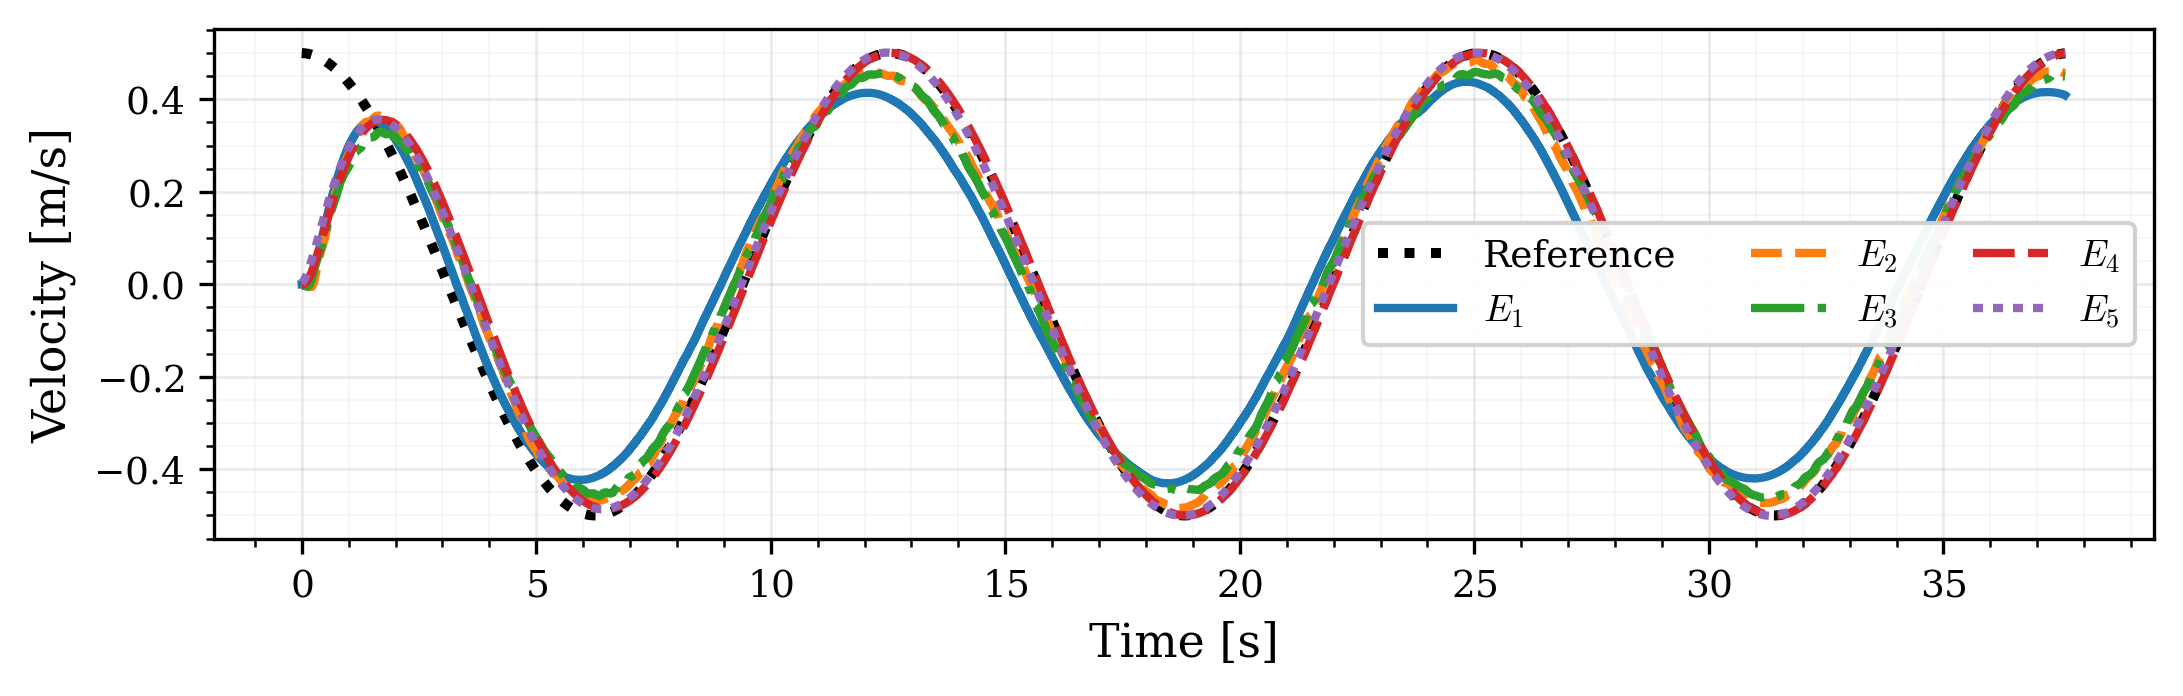
\includegraphics[width=\linewidth]{experiment_plots/tracking_velocity_x.png}\caption{$v_x(t)$.}\end{subfigure}
    \\
    \begin{subfigure}{\textwidth}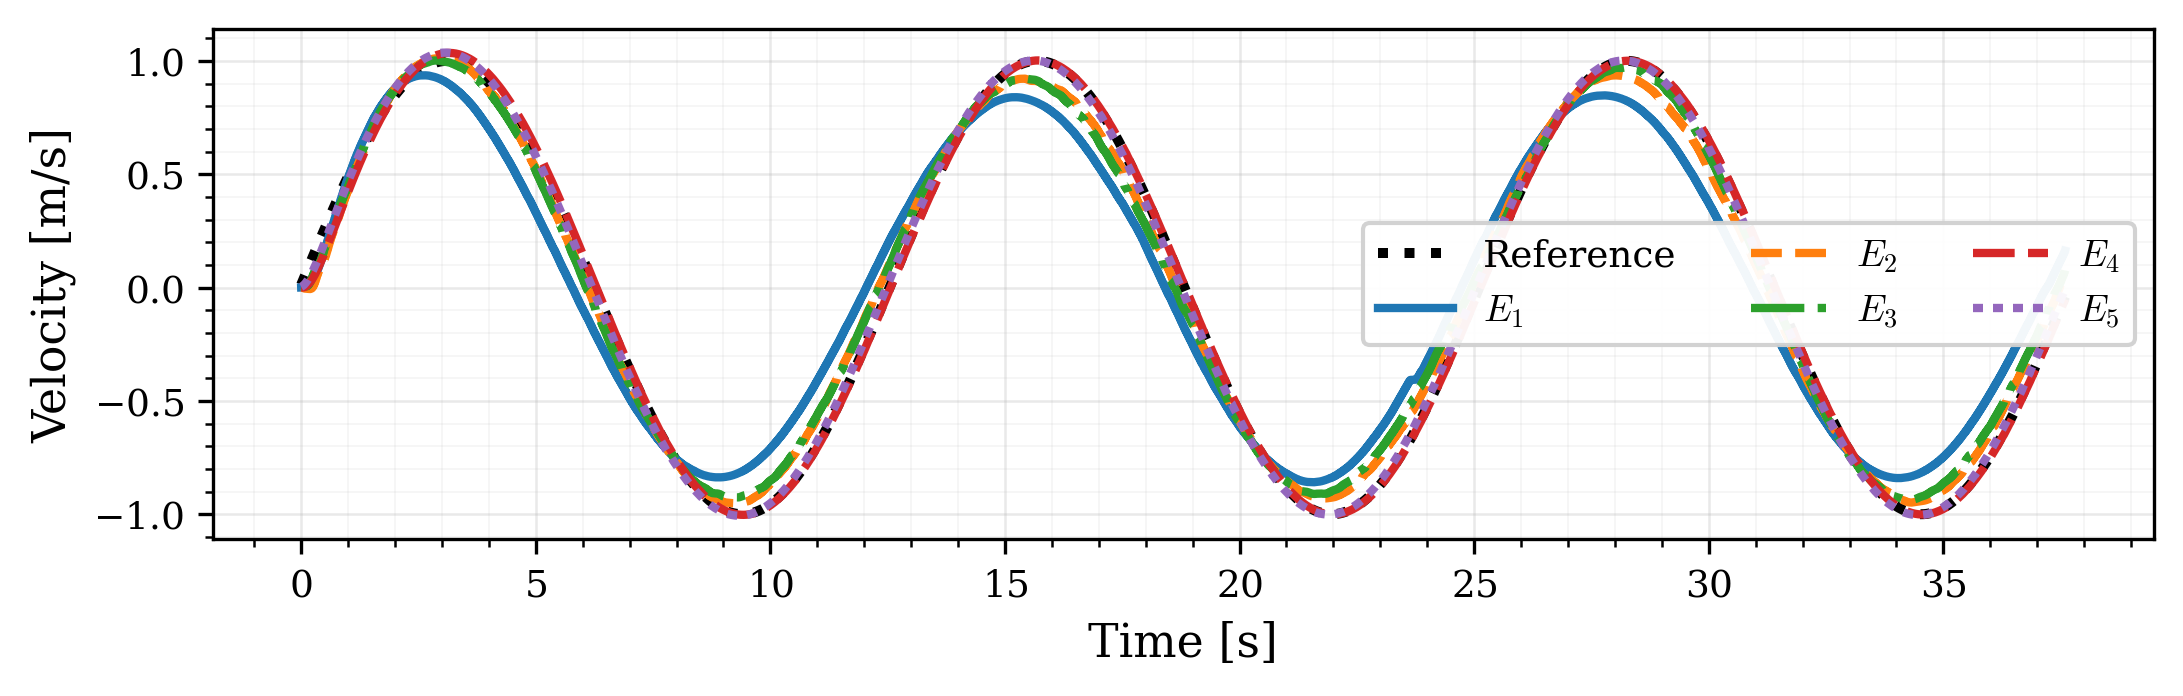
\includegraphics[width=\linewidth]{experiment_plots/tracking_velocity_y.png}\caption{$v_y(t)$.}\end{subfigure}
    \\
    \begin{subfigure}{\textwidth}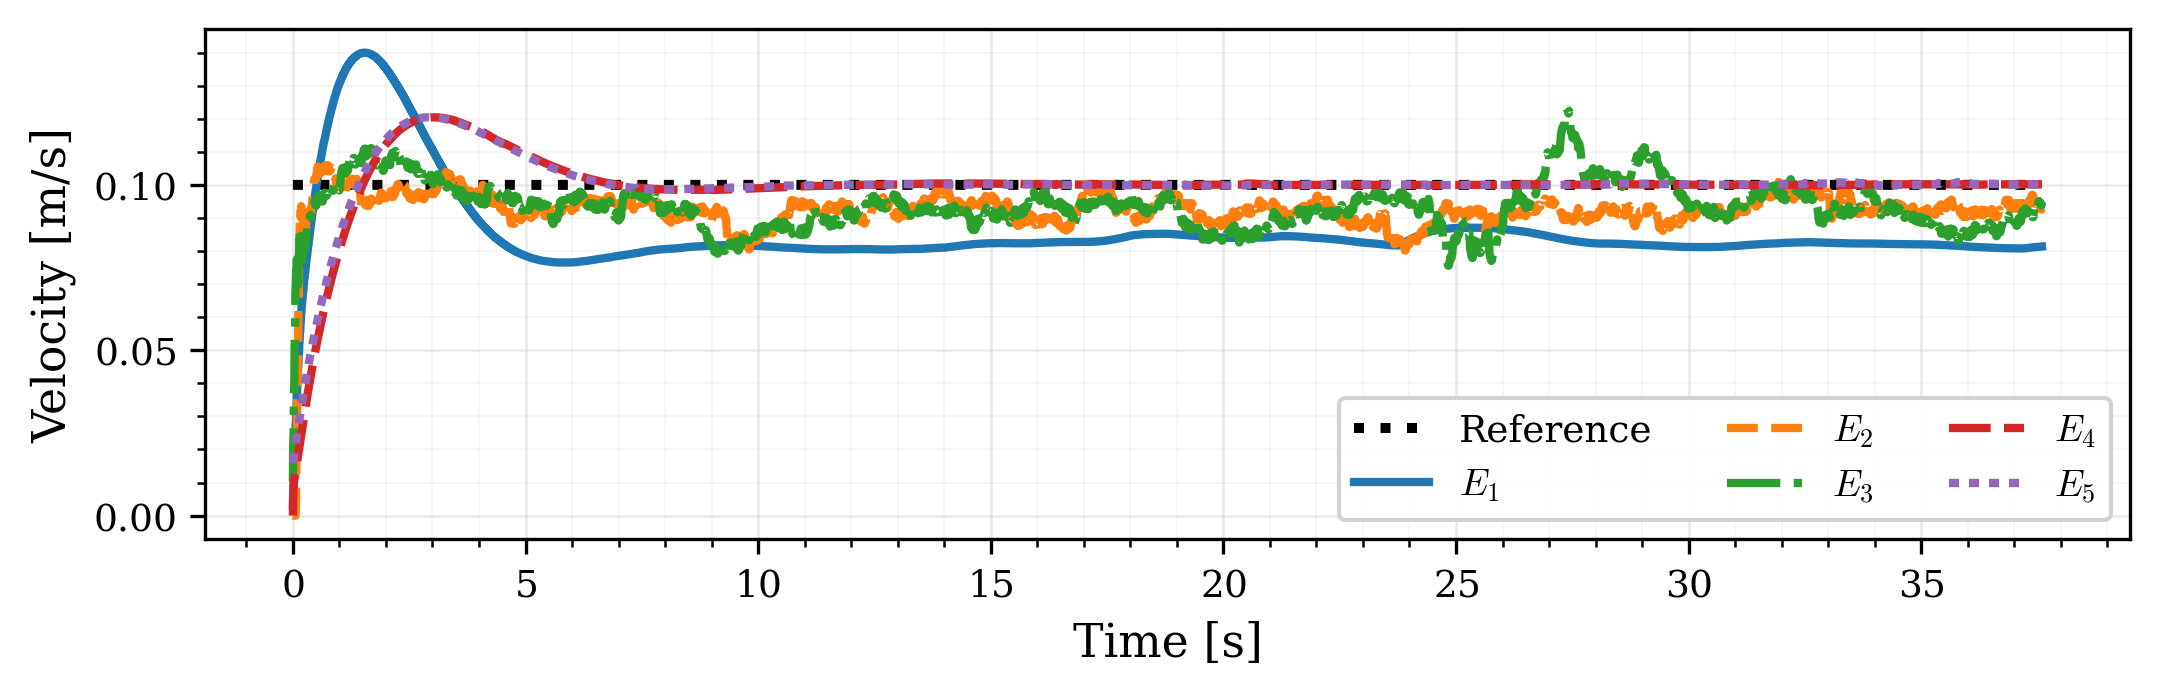
\includegraphics[width=\linewidth]{experiment_plots/tracking_velocity_z.png}\caption{$v_z(t)$.}\end{subfigure}
    \caption{Per-axis velocity tracking.}
    \label{fig:app-tracking-velocity}
\end{figure}

\subsection{Per-Axis Velocity Error}
\begin{figure}[H]
    \centering
    \begin{subfigure}{\textwidth}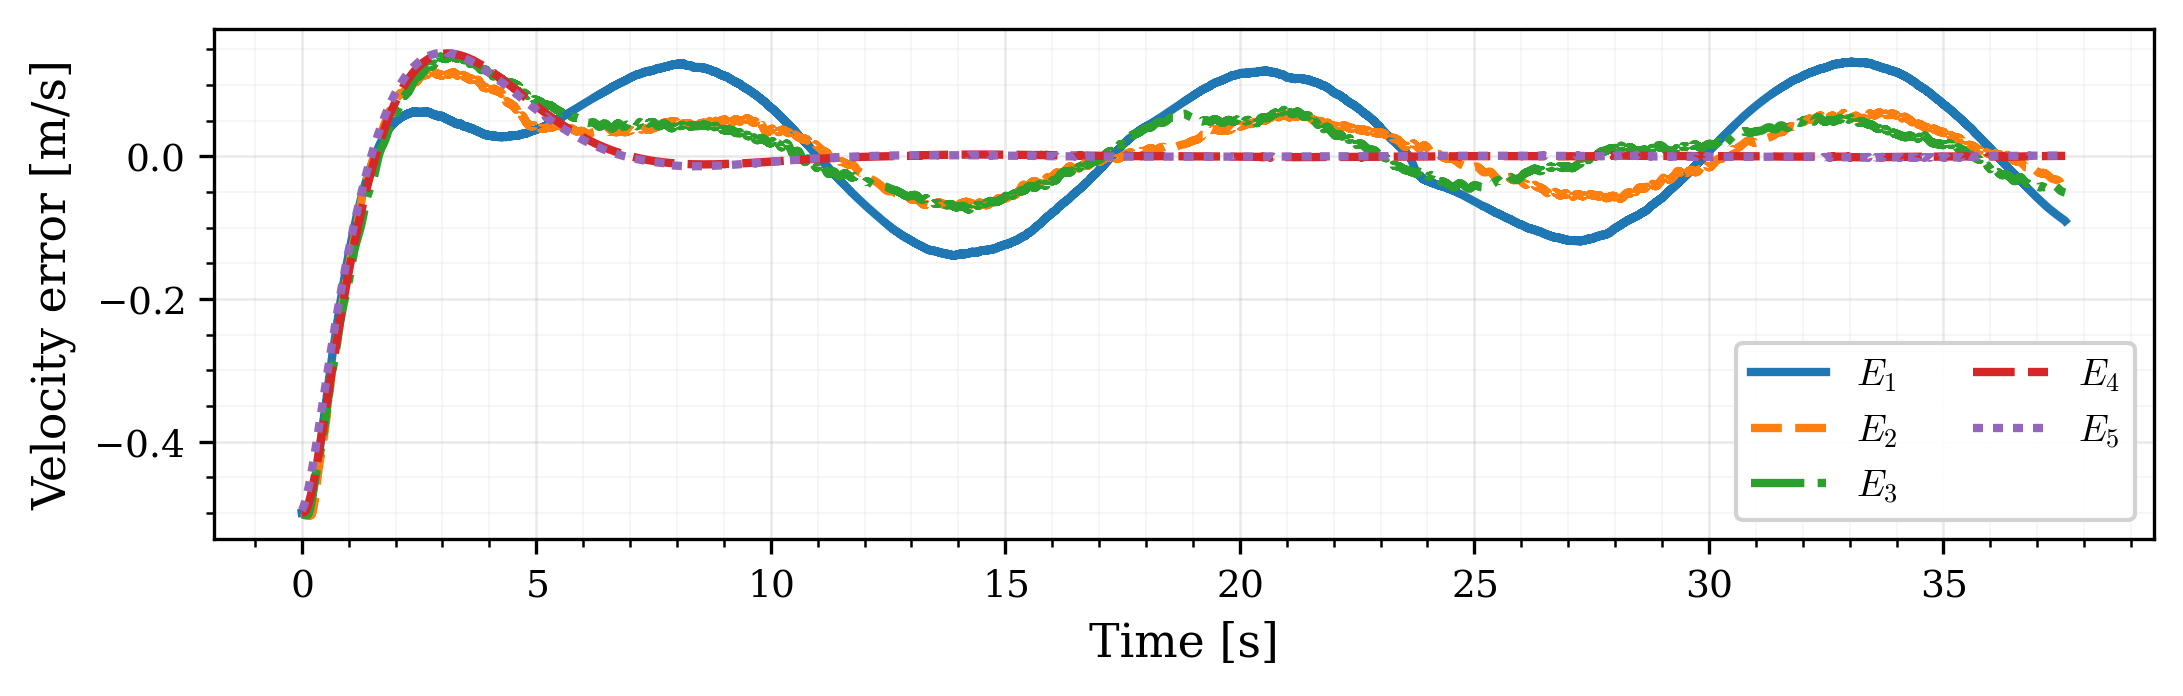
\includegraphics[width=\linewidth]{experiment_plots/error_velocity_x.png}\caption{$e_{v,1}(t)$.}\end{subfigure}
    \\
    \begin{subfigure}{\textwidth}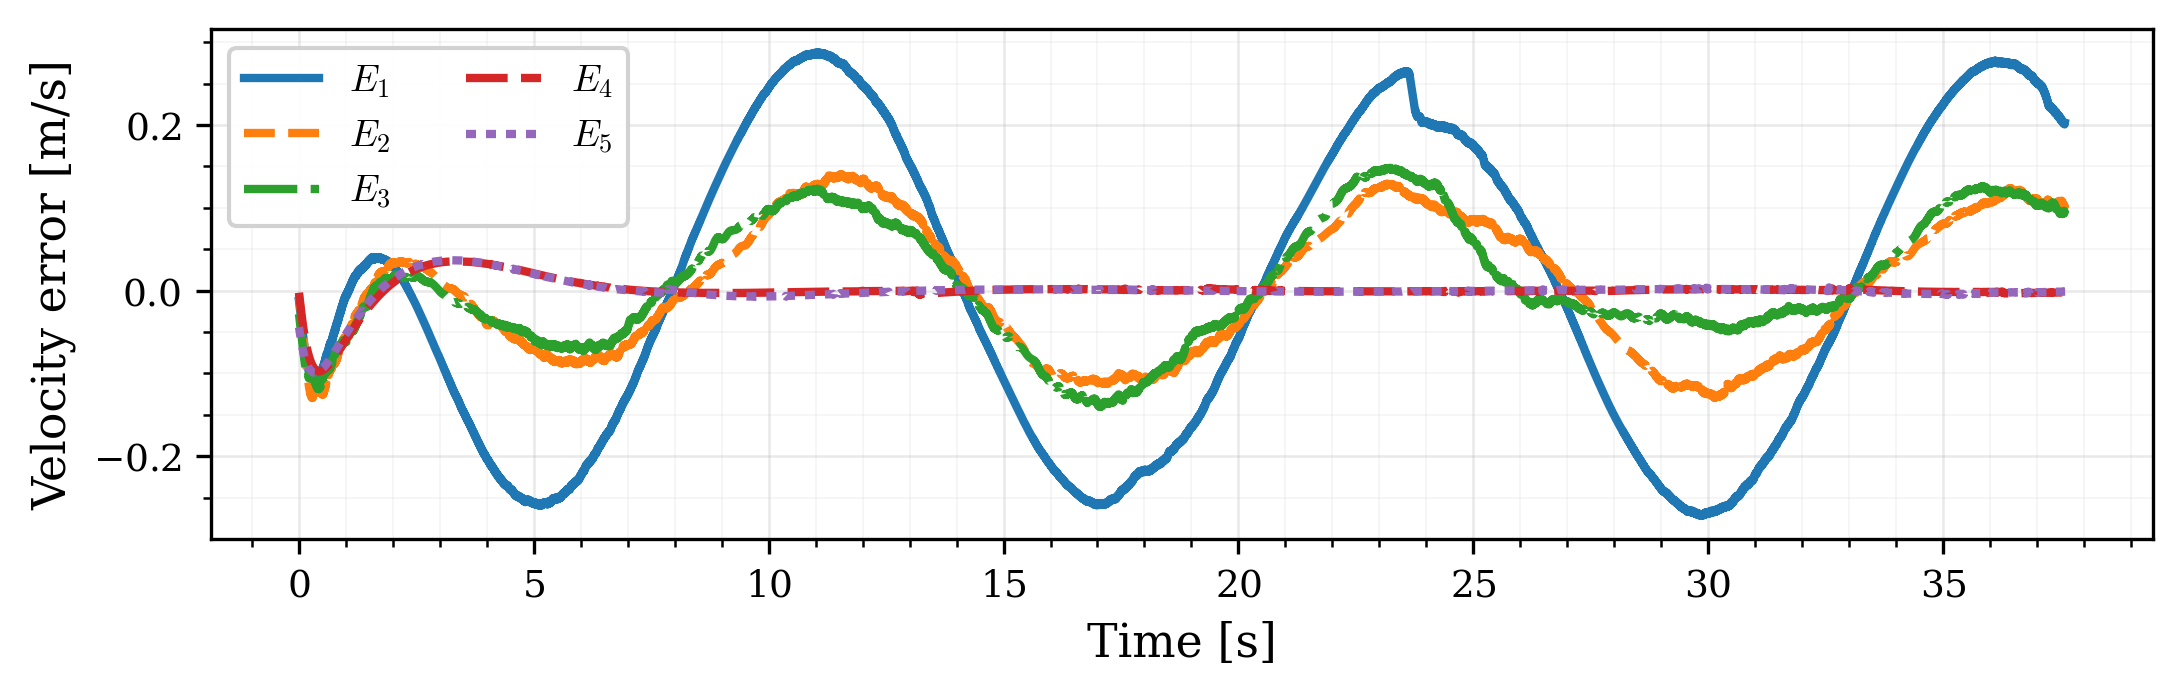
\includegraphics[width=\linewidth]{experiment_plots/error_velocity_y.png}\caption{$e_{v,2}(t)$.}\end{subfigure}
    \\
    \begin{subfigure}{\textwidth}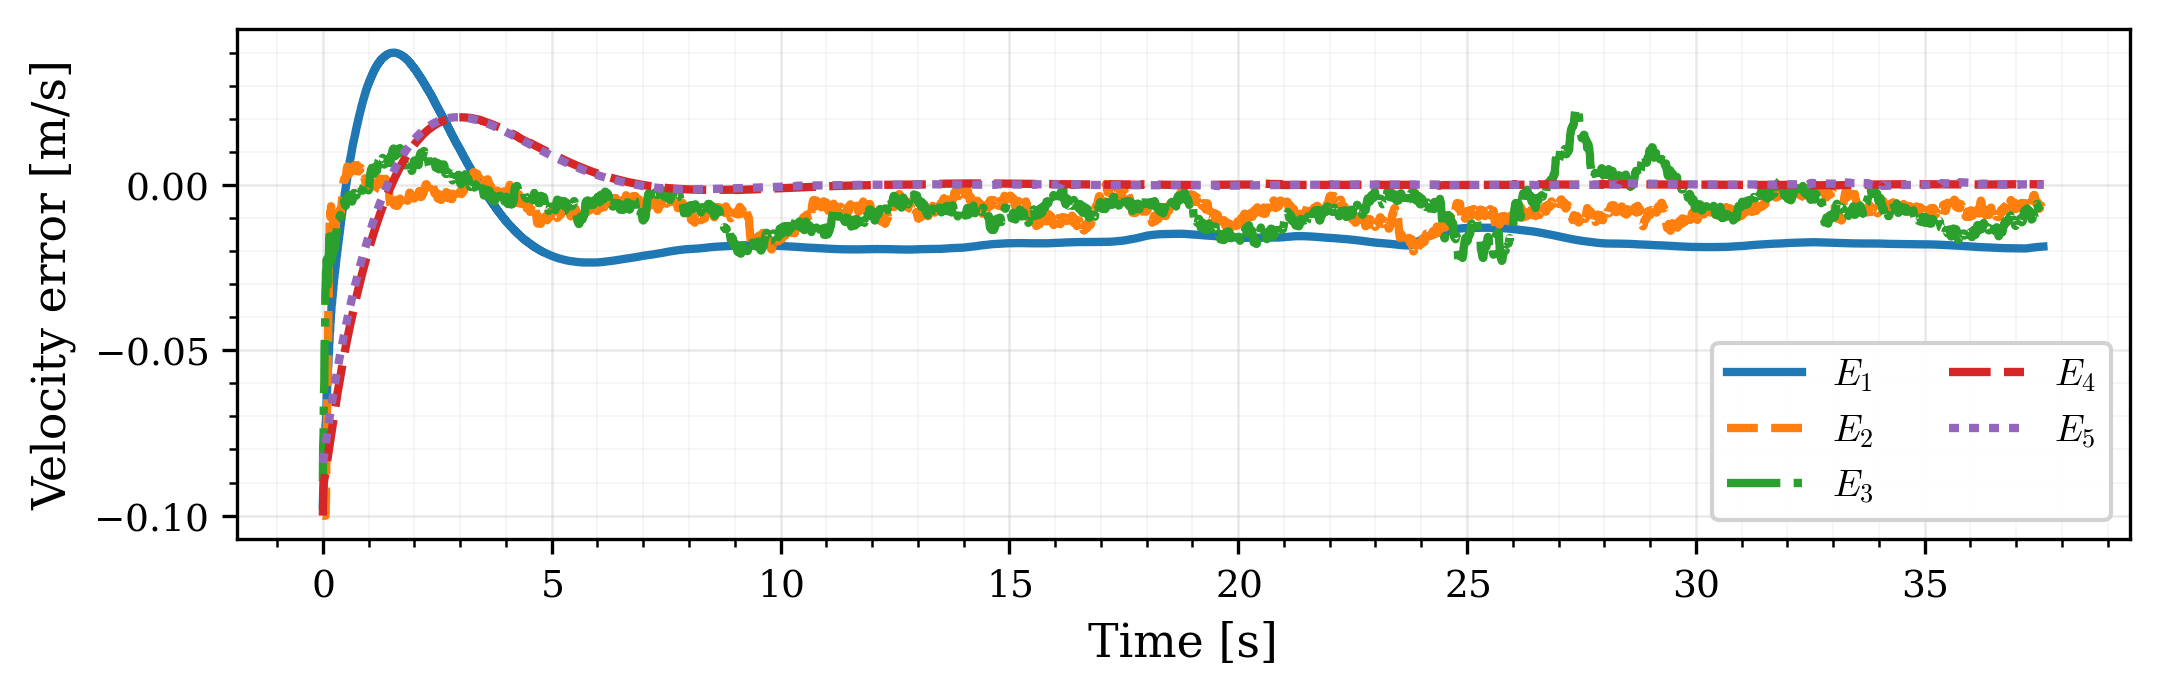
\includegraphics[width=\linewidth]{experiment_plots/error_velocity_z.png}\caption{$e_{v,3}(t)$.}\end{subfigure}
    \caption{Velocity-error components per inertial axis.}
    \label{fig:app-error-velocity}
\end{figure}

\subsection{Per-Axis Acceleration Tracking}
\begin{figure}[H]
    \centering
    \begin{subfigure}{\textwidth}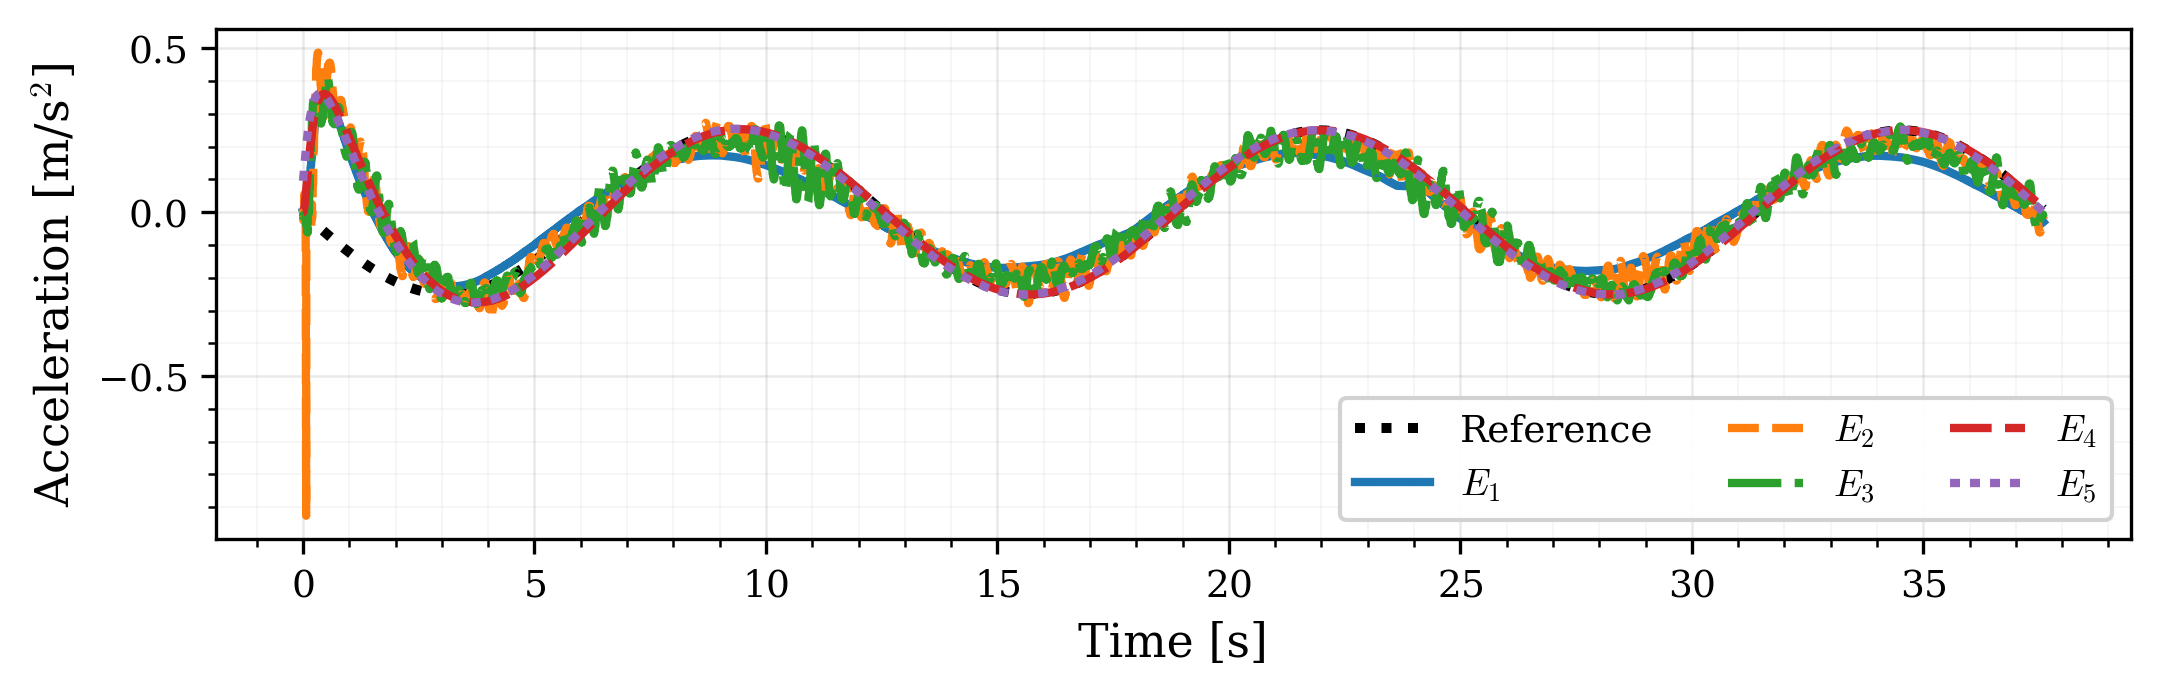
\includegraphics[width=\linewidth]{experiment_plots/tracking_acceleration_x.png}\caption{$a_x(t)$.}\end{subfigure}
    \\
    \begin{subfigure}{\textwidth}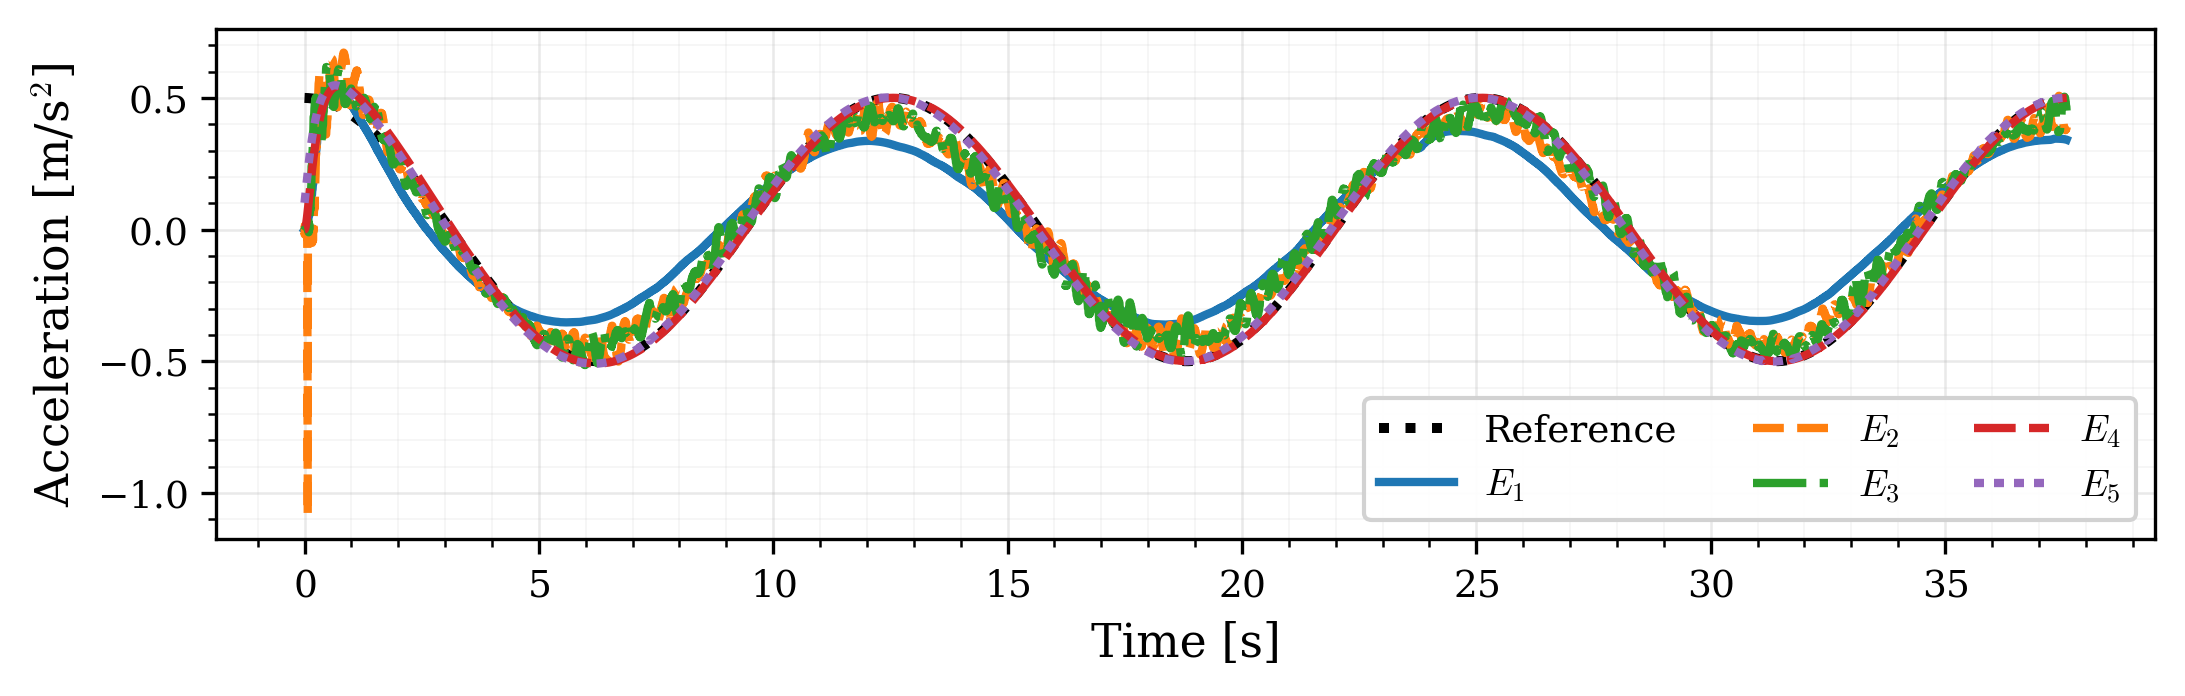
\includegraphics[width=\linewidth]{experiment_plots/tracking_acceleration_y.png}\caption{$a_y(t)$.}\end{subfigure}
    \\
    \begin{subfigure}{\textwidth}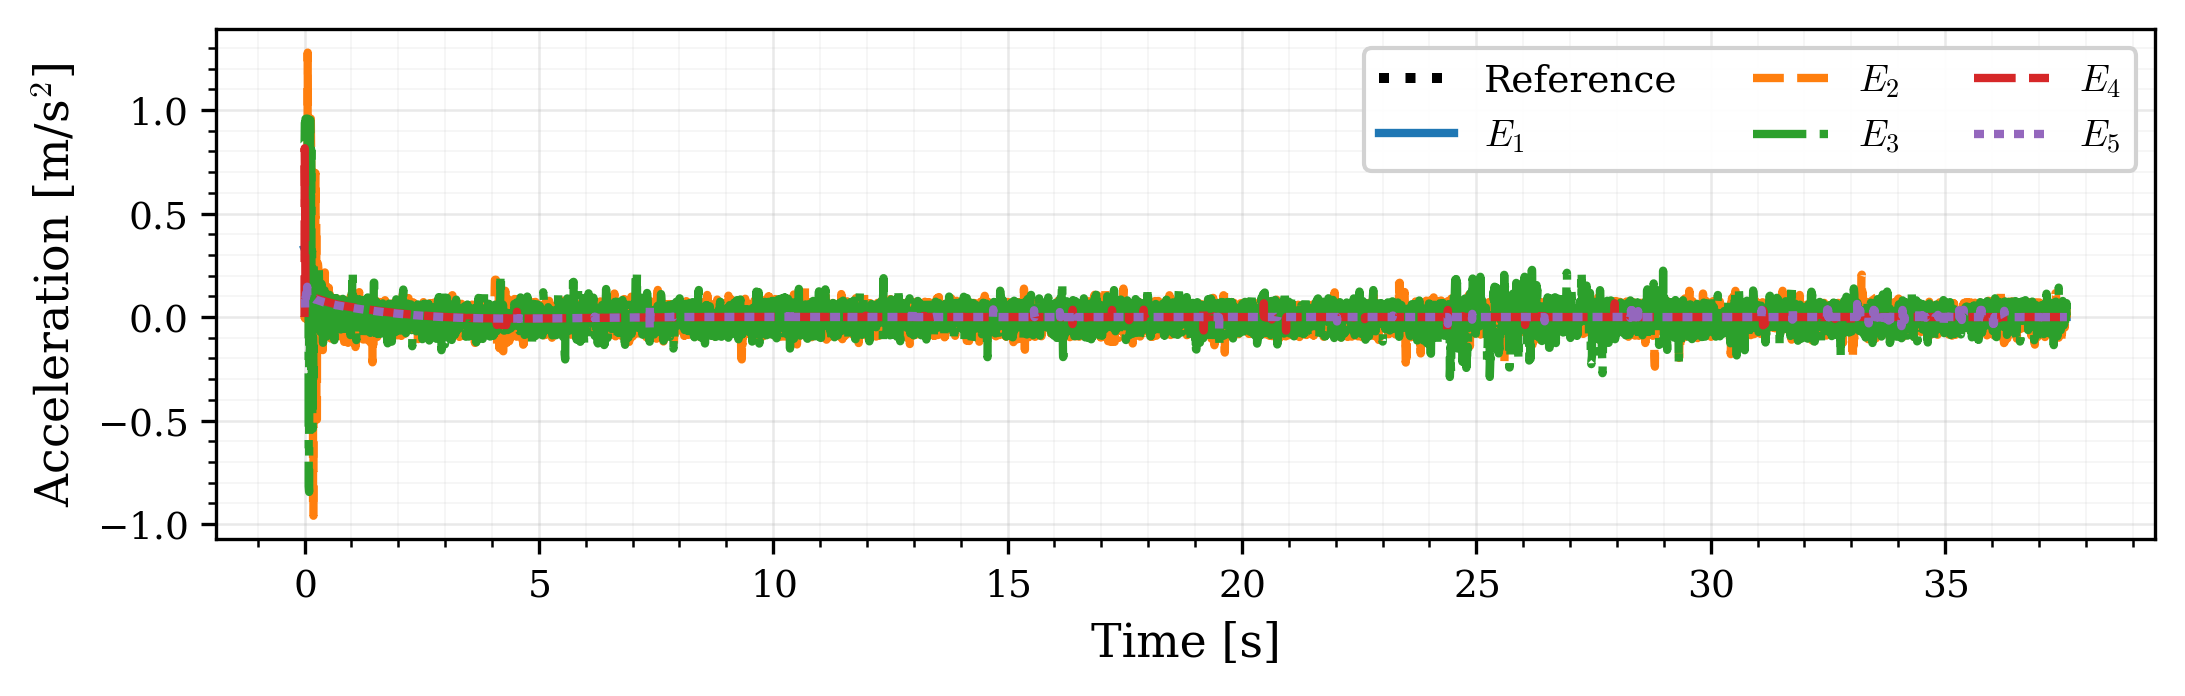
\includegraphics[width=\linewidth]{experiment_plots/tracking_acceleration_z.png}\caption{$a_z(t)$.}\end{subfigure}
    \caption{Per-axis acceleration tracking.}
    \label{fig:app-tracking-accel}
\end{figure}

\subsection{Per-Axis Acceleration Error}
\begin{figure}[H]
    \centering
    \begin{subfigure}{\textwidth}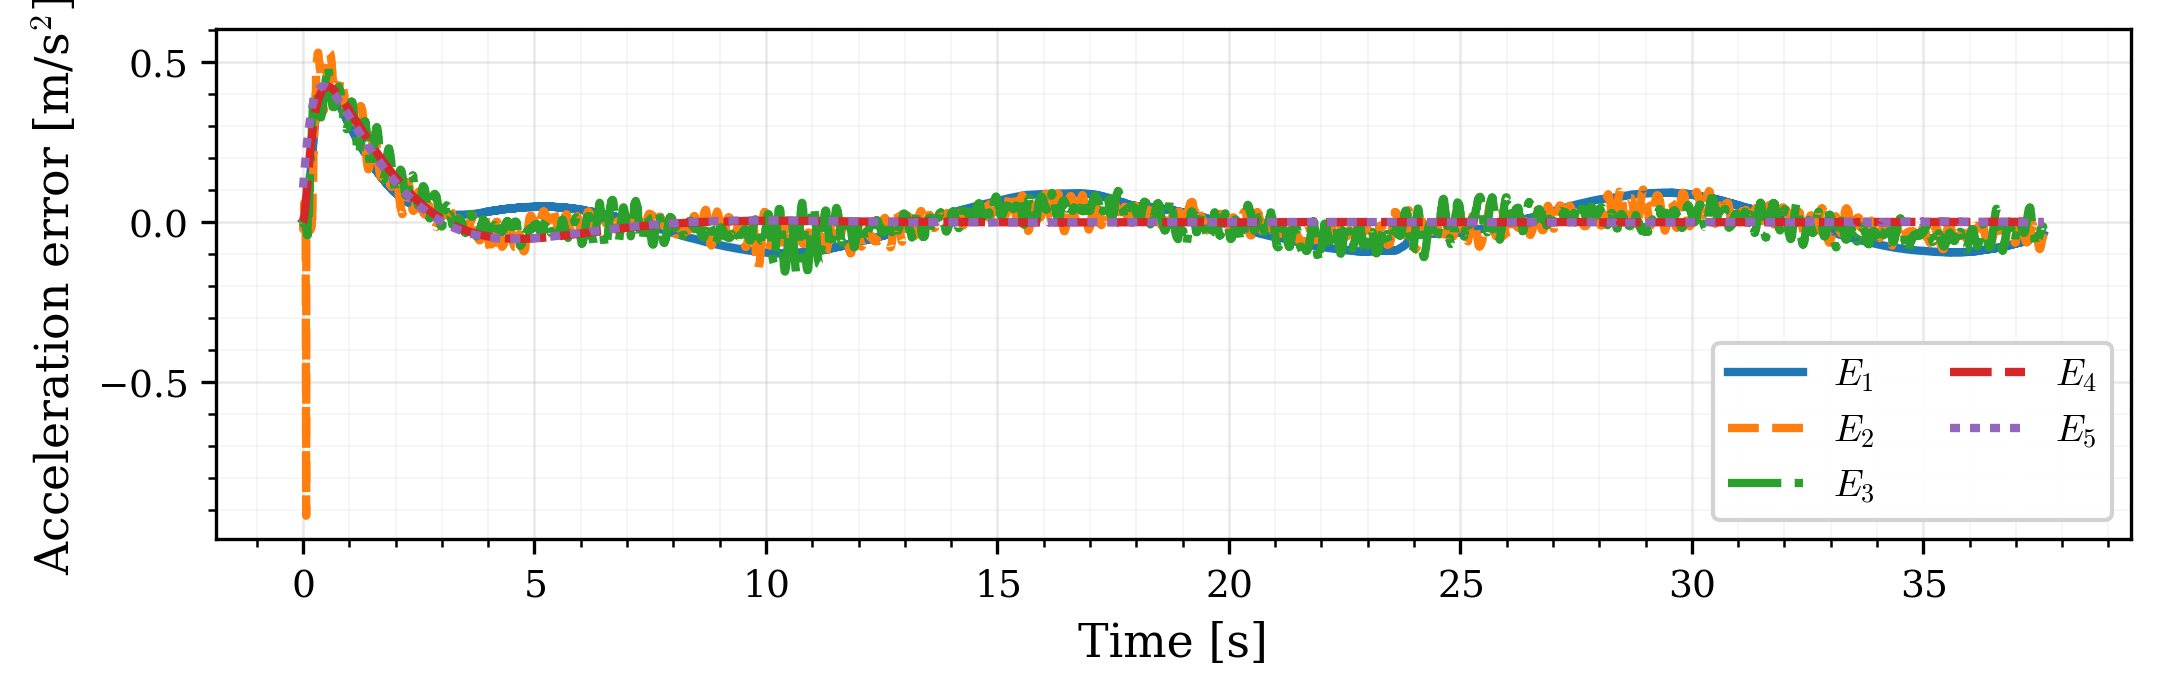
\includegraphics[width=\linewidth]{experiment_plots/error_acceleration_x.png}\caption{$\dot e_{v,1}(t)$.}\end{subfigure}
    \\
    \begin{subfigure}{\textwidth}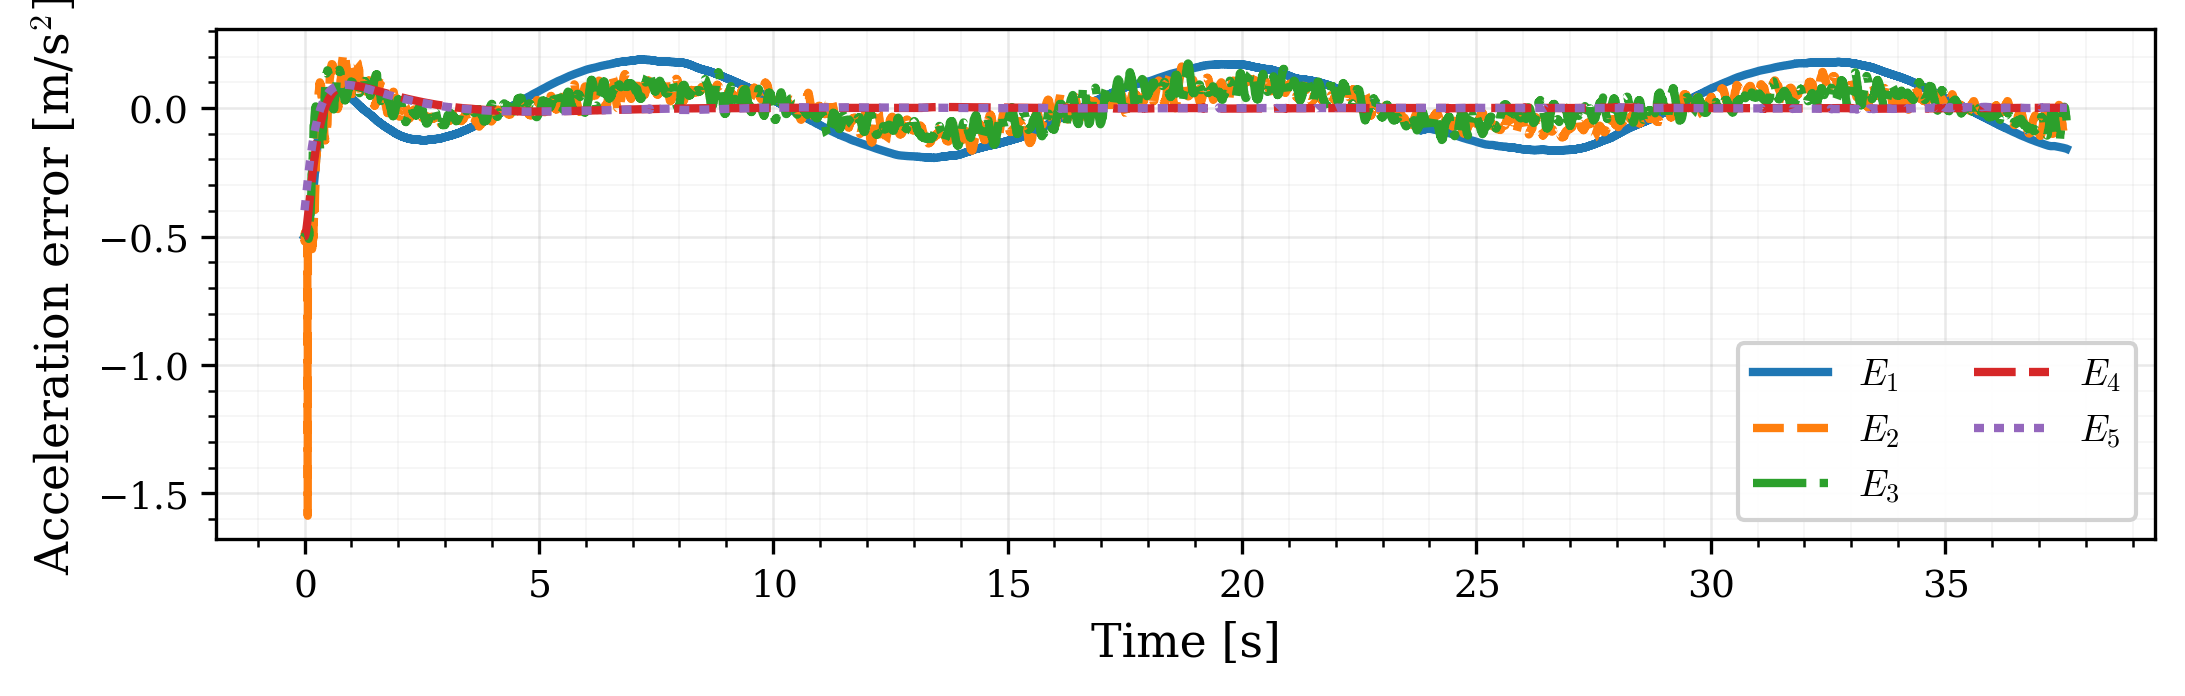
\includegraphics[width=\linewidth]{experiment_plots/error_acceleration_y.png}\caption{$\dot e_{v,2}(t)$.}\end{subfigure}
    \\
    \begin{subfigure}{\textwidth}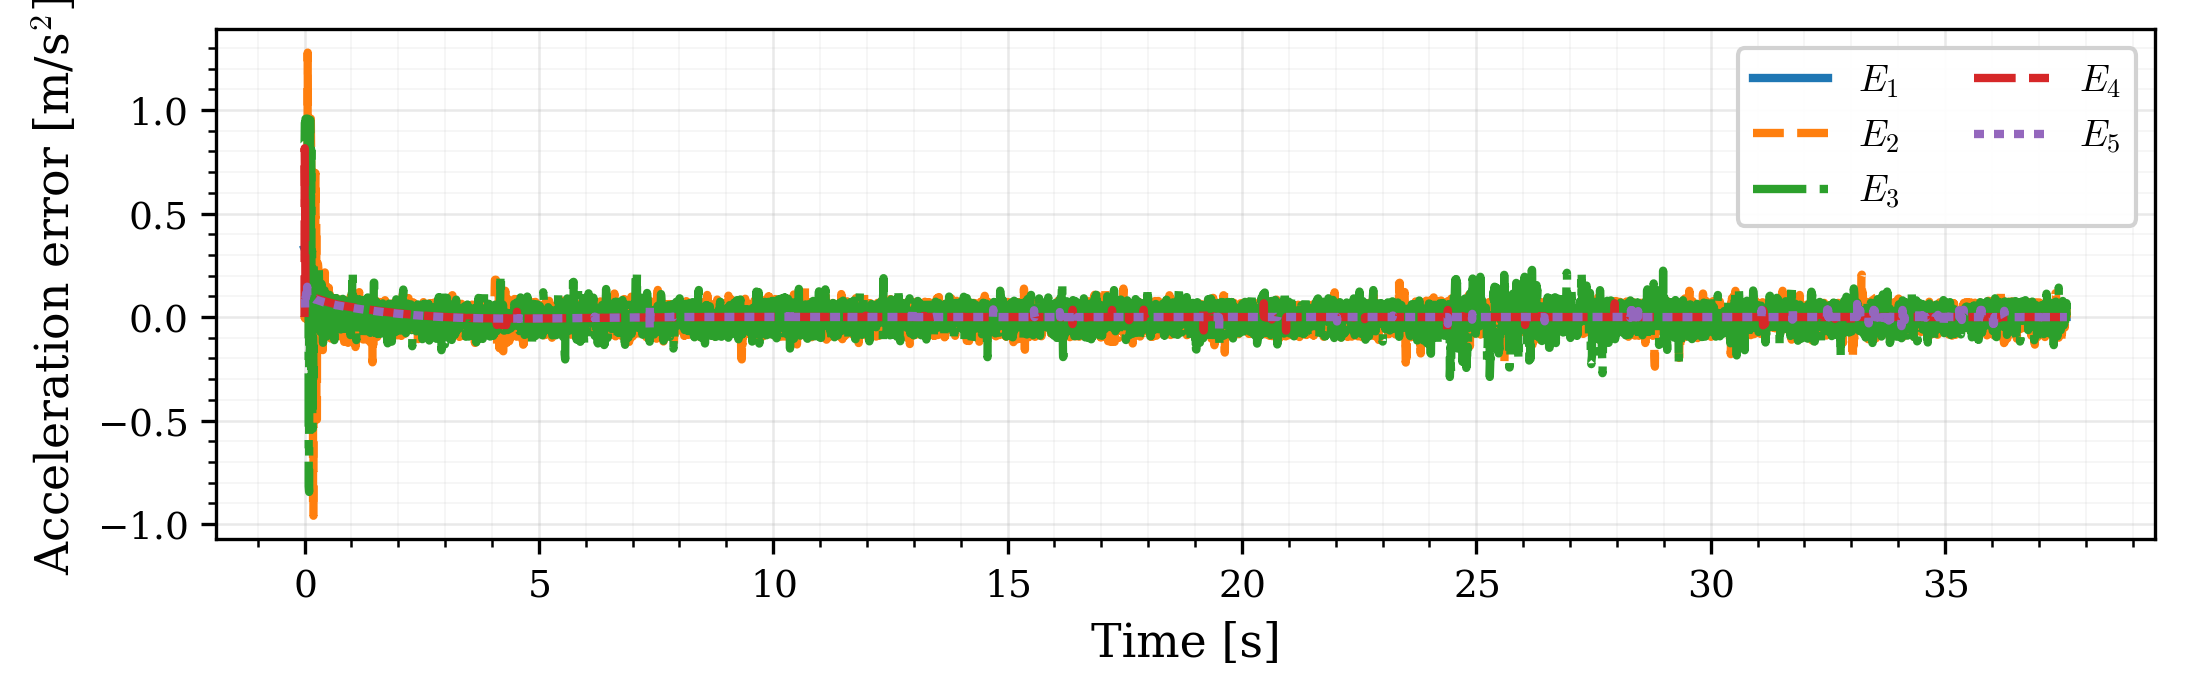
\includegraphics[width=\linewidth]{experiment_plots/error_acceleration_z.png}\caption{$\dot e_{v,3}(t)$.}\end{subfigure}
    \caption{Acceleration-error components per inertial axis.}
    \label{fig:app-error-accel}
\end{figure}

\subsection{Per-Axis Attitude-Error Components}
\begin{figure}[H]
    \centering
    \begin{subfigure}{\textwidth}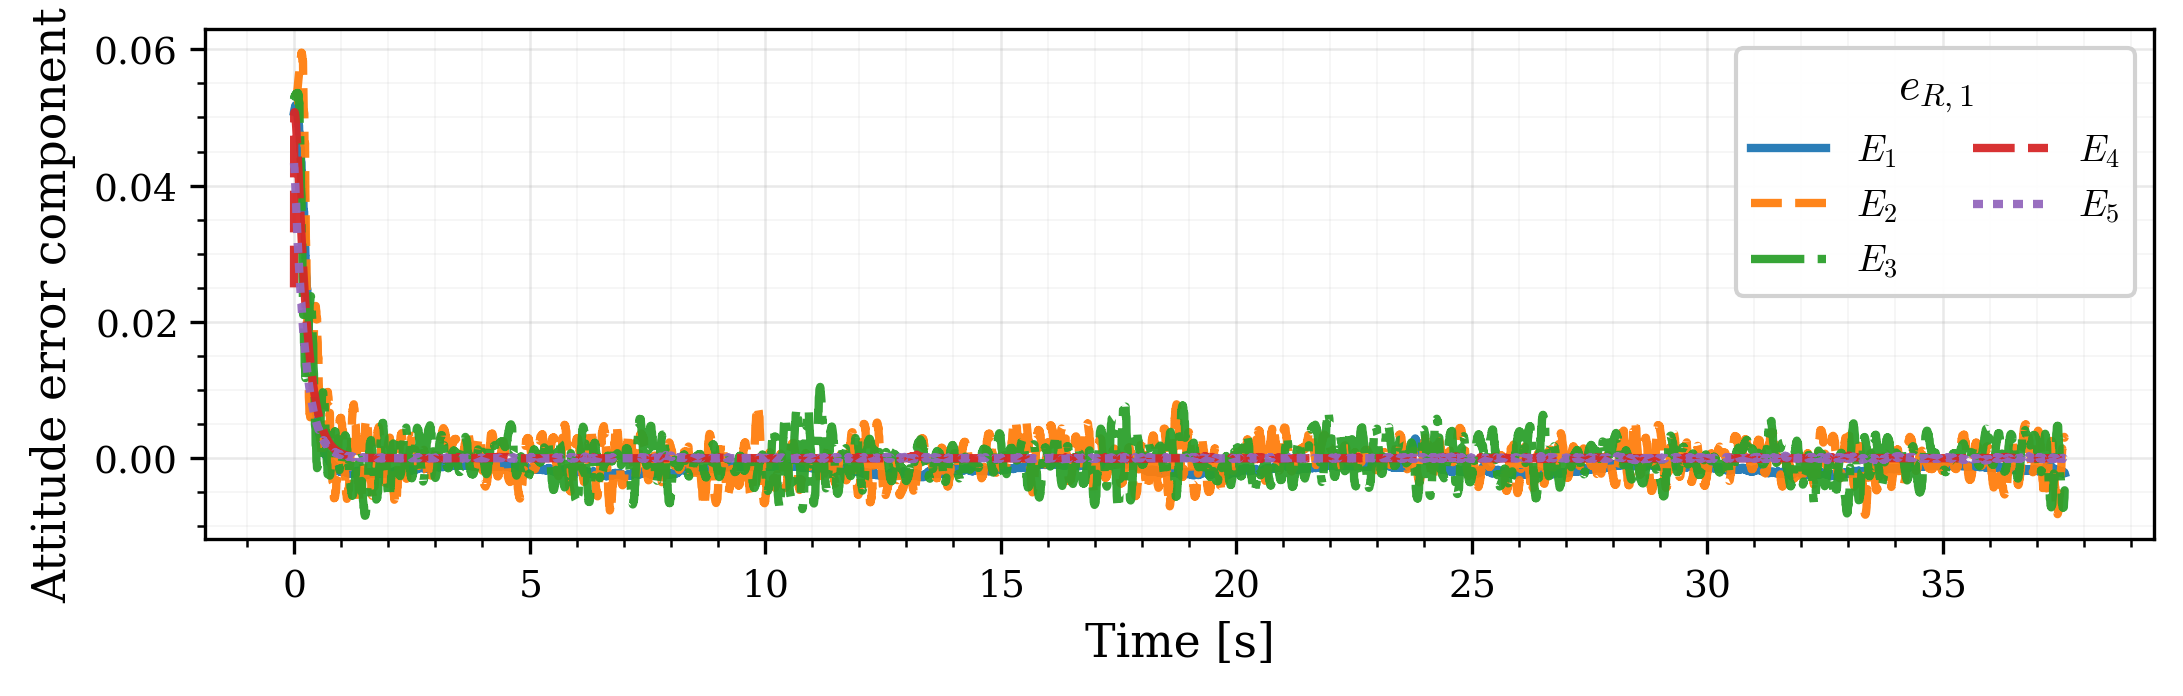
\includegraphics[width=\linewidth]{experiment_plots/error_attitude_component_x.png}\caption{$e_{R,1}(t)$.}\end{subfigure}
    \\
    \begin{subfigure}{\textwidth}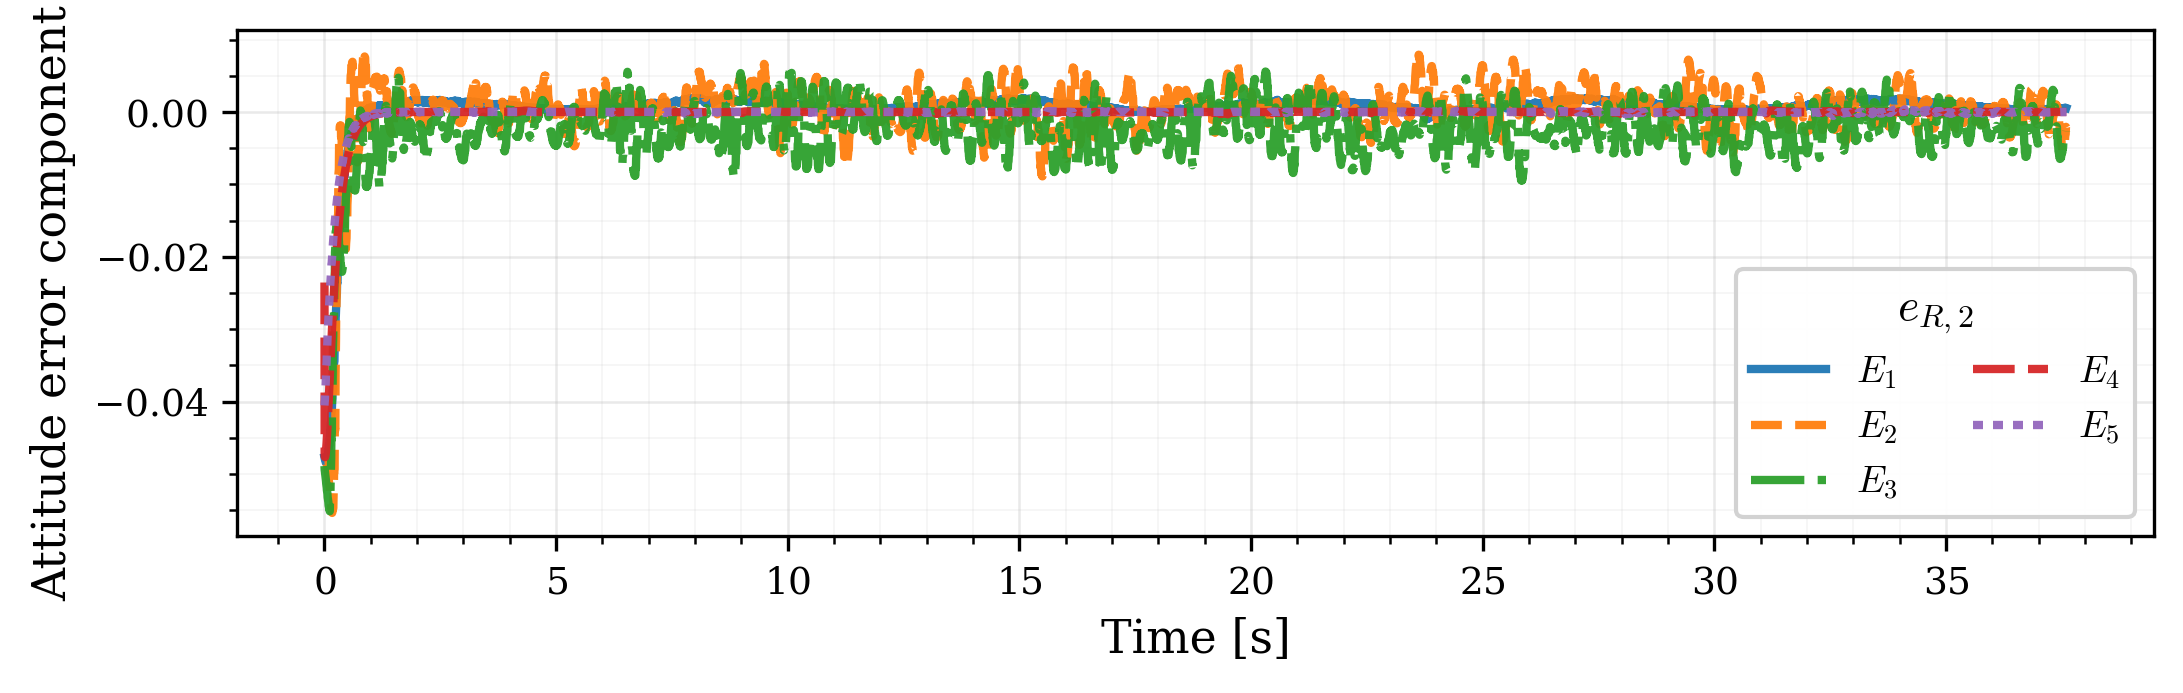
\includegraphics[width=\linewidth]{experiment_plots/error_attitude_component_y.png}\caption{$e_{R,2}(t)$.}\end{subfigure}
    \\
    \begin{subfigure}{\textwidth}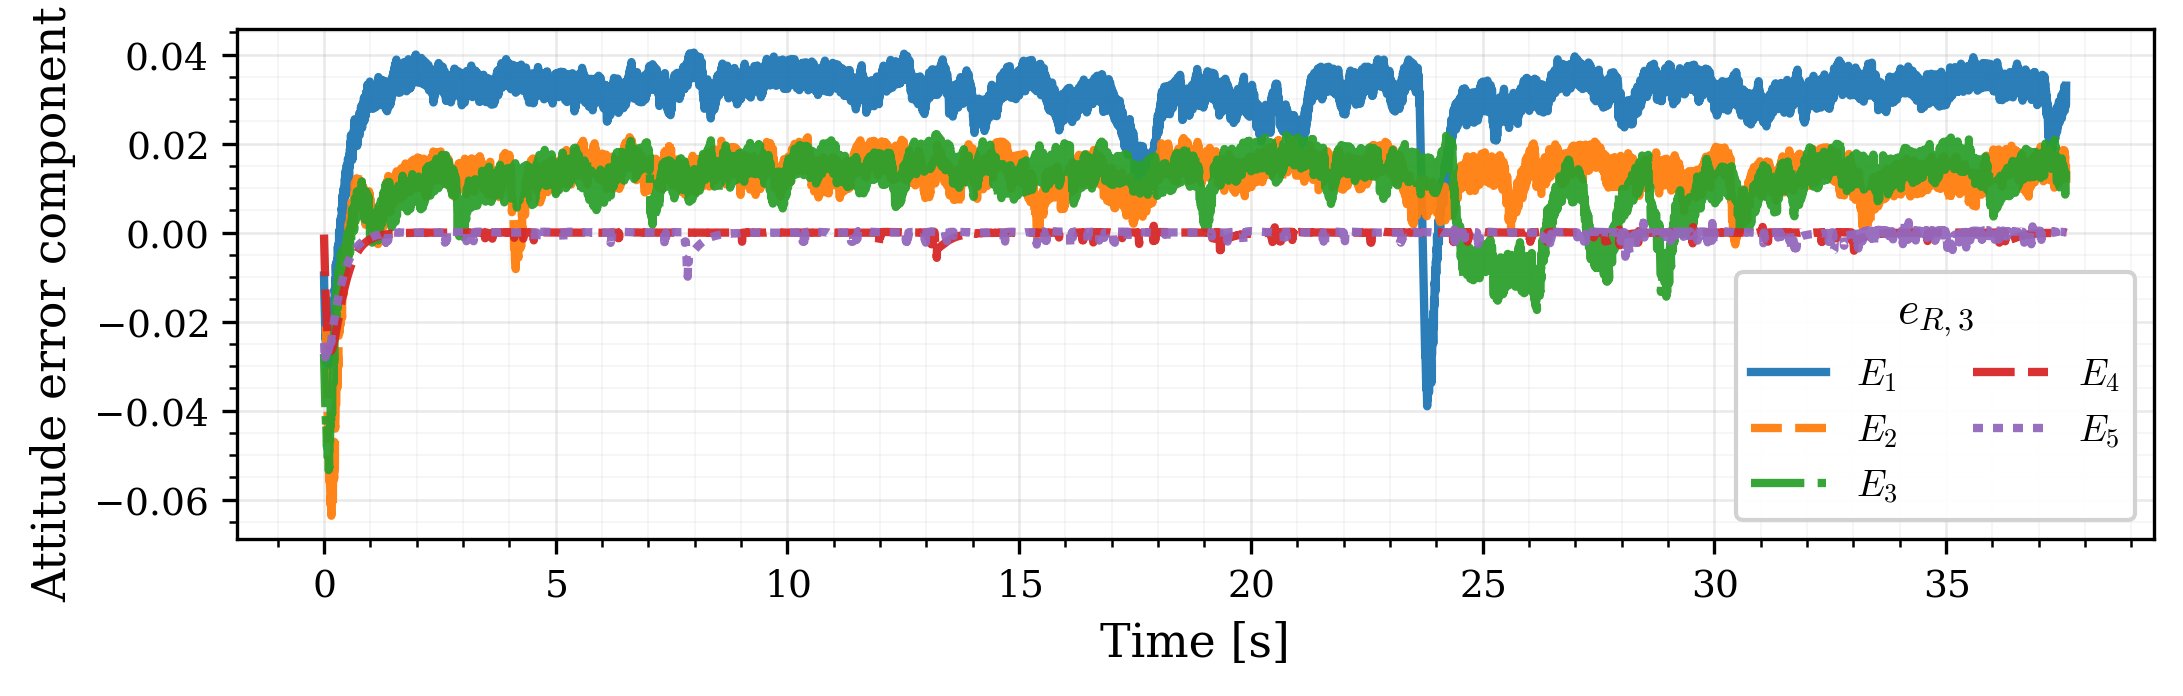
\includegraphics[width=\linewidth]{experiment_plots/error_attitude_component_z.png}\caption{$e_{R,3}(t)$.}\end{subfigure}
    \caption{Per-body-axis components of the attitude error vector $e_R$.}
    \label{fig:app-error-eR-axes}
\end{figure}

\subsection{Per-Axis Angular-Rate Tracking}
\begin{figure}[H]
    \centering
    \begin{subfigure}{\textwidth}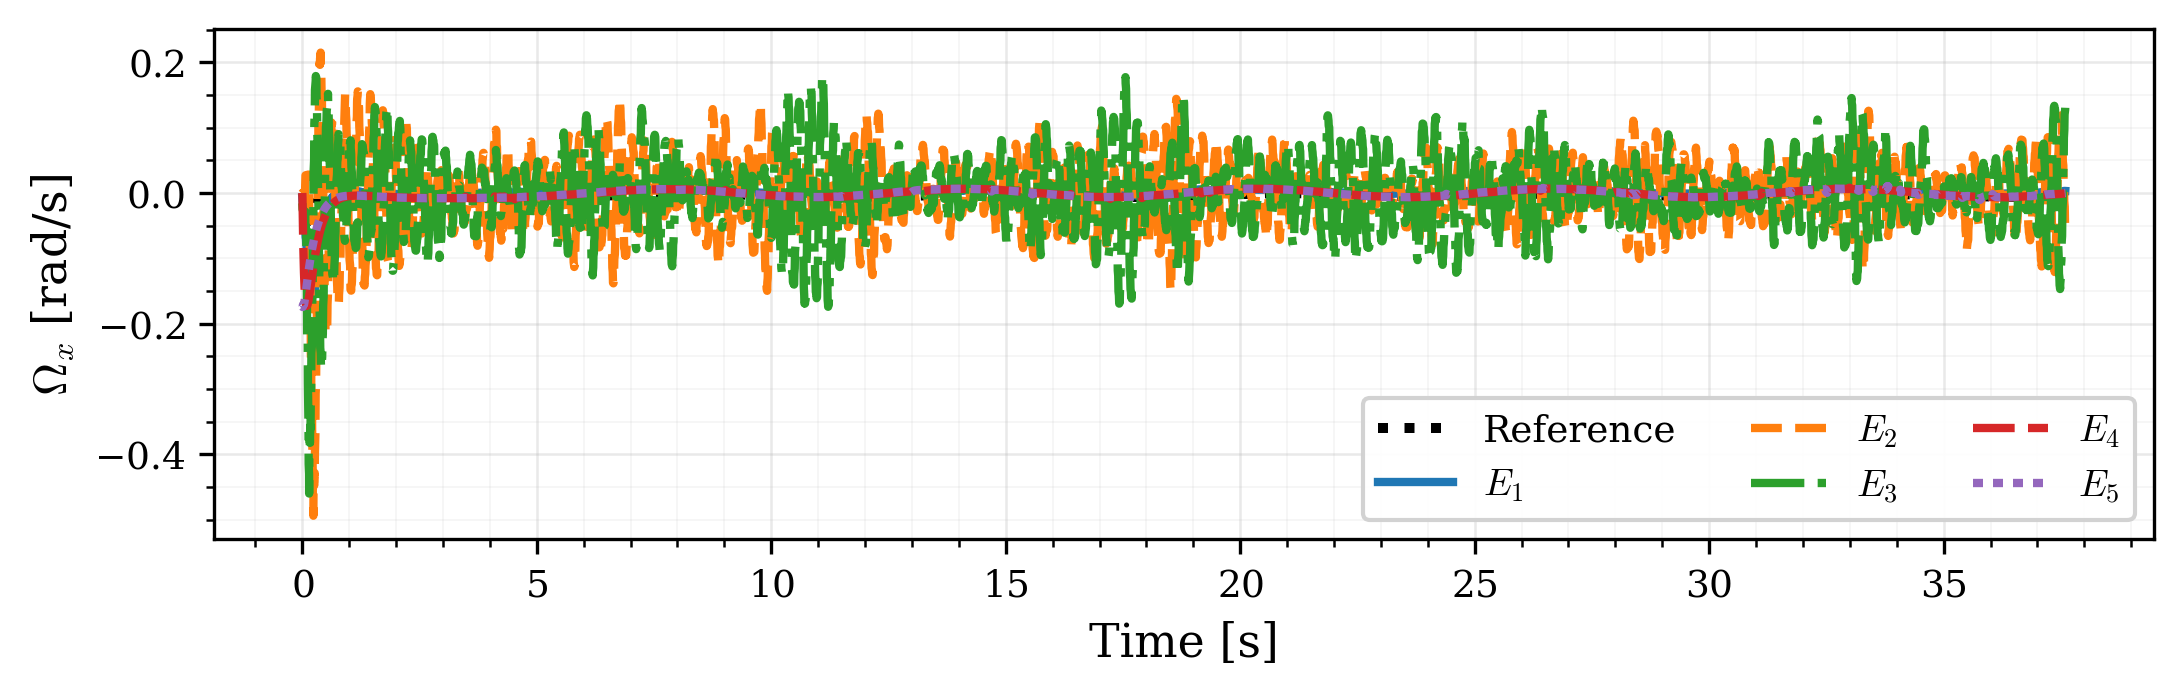
\includegraphics[width=\linewidth]{experiment_plots/tracking_omega_x.png}\caption{$\Omega_x(t)$.}\end{subfigure}
    \\
    \begin{subfigure}{\textwidth}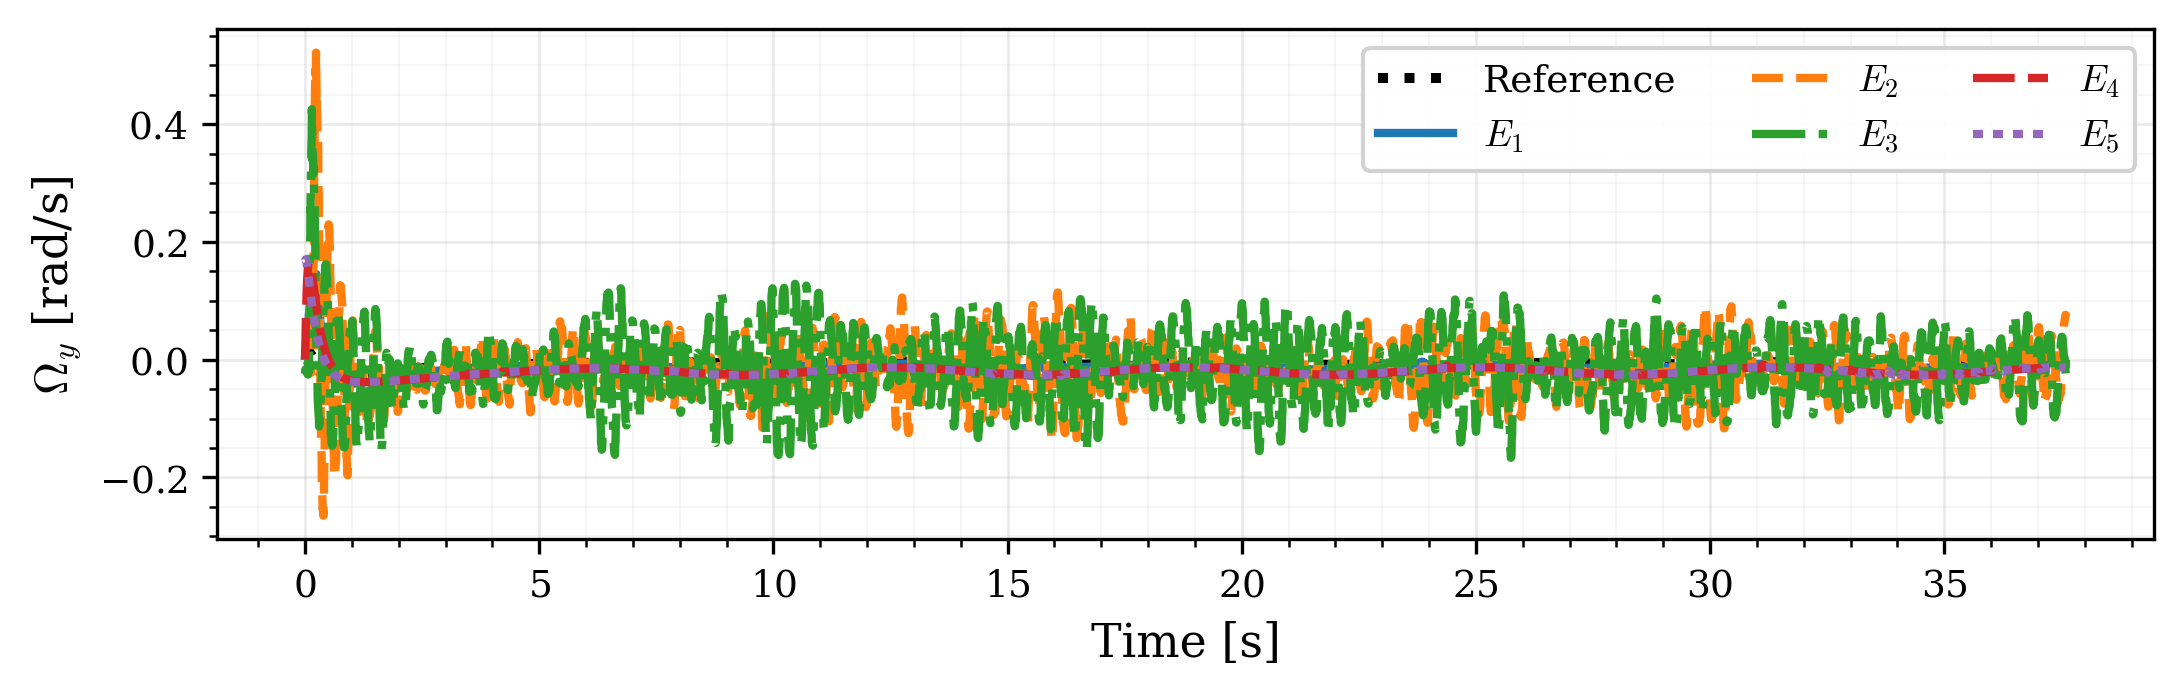
\includegraphics[width=\linewidth]{experiment_plots/tracking_omega_y.png}\caption{$\Omega_y(t)$.}\end{subfigure}
    \\
    \begin{subfigure}{\textwidth}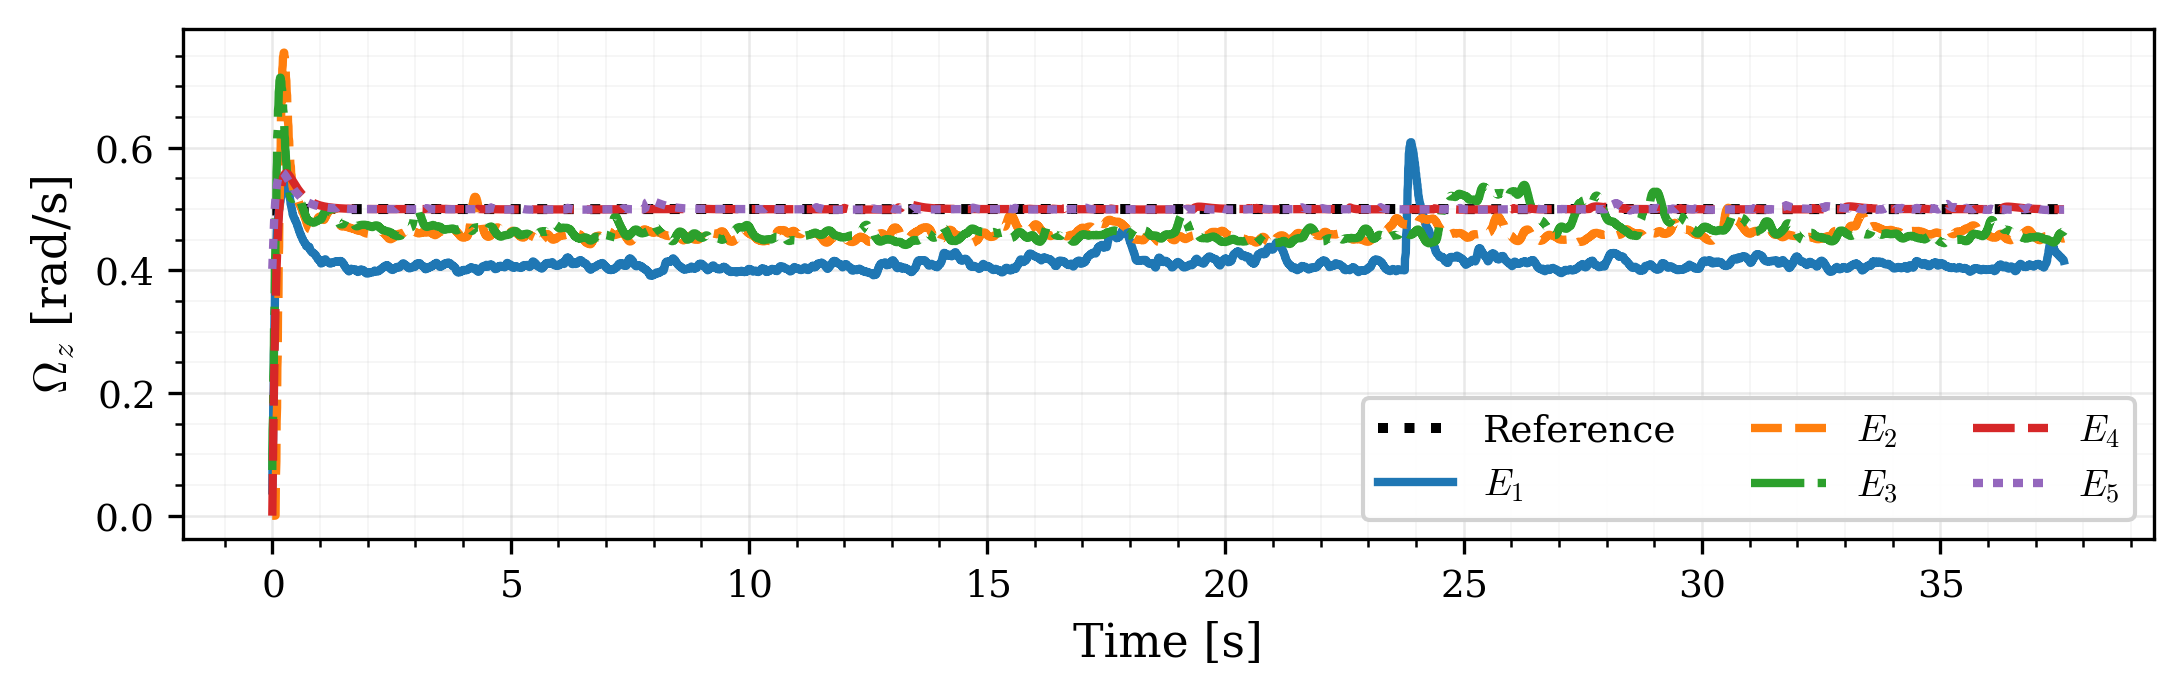
\includegraphics[width=\linewidth]{experiment_plots/tracking_omega_z.png}\caption{$\Omega_z(t)$.}\end{subfigure}
    \caption{Per-body-axis angular-rate tracking.}
    \label{fig:app-tracking-omega}
\end{figure}

\subsection{Per-Axis Angular-Velocity-Error Components}
\begin{figure}[H]
    \centering
    \begin{subfigure}{\textwidth}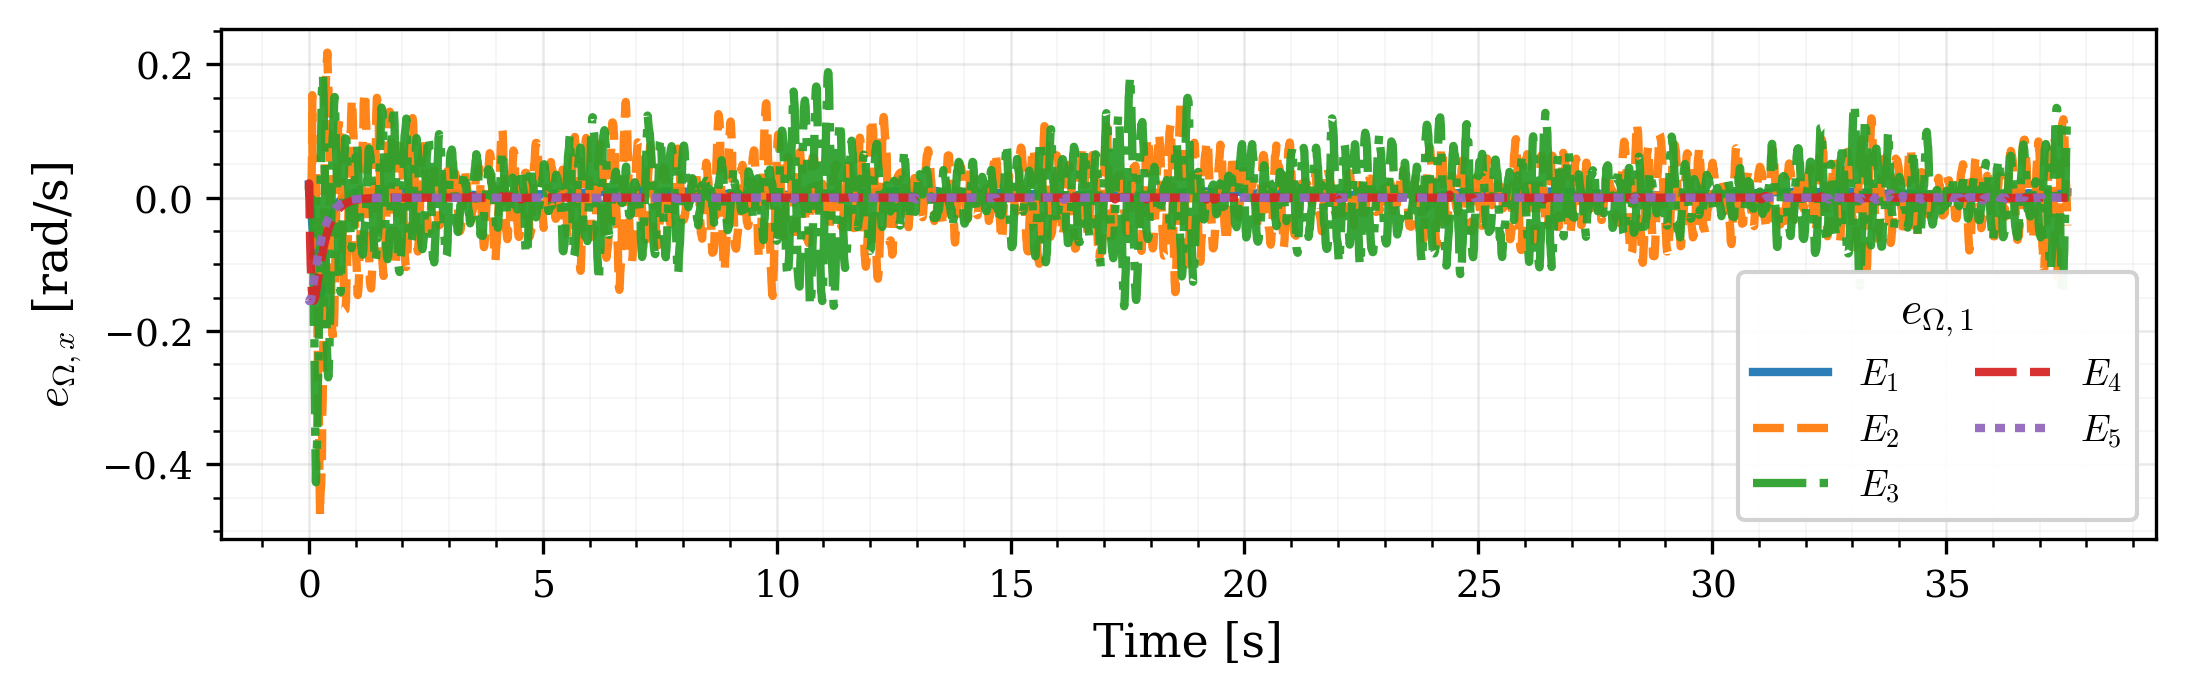
\includegraphics[width=\linewidth]{experiment_plots/error_angular_velocity_component_x.png}\caption{$e_{\Omega,1}(t)$.}\end{subfigure}
    \\
    \begin{subfigure}{\textwidth}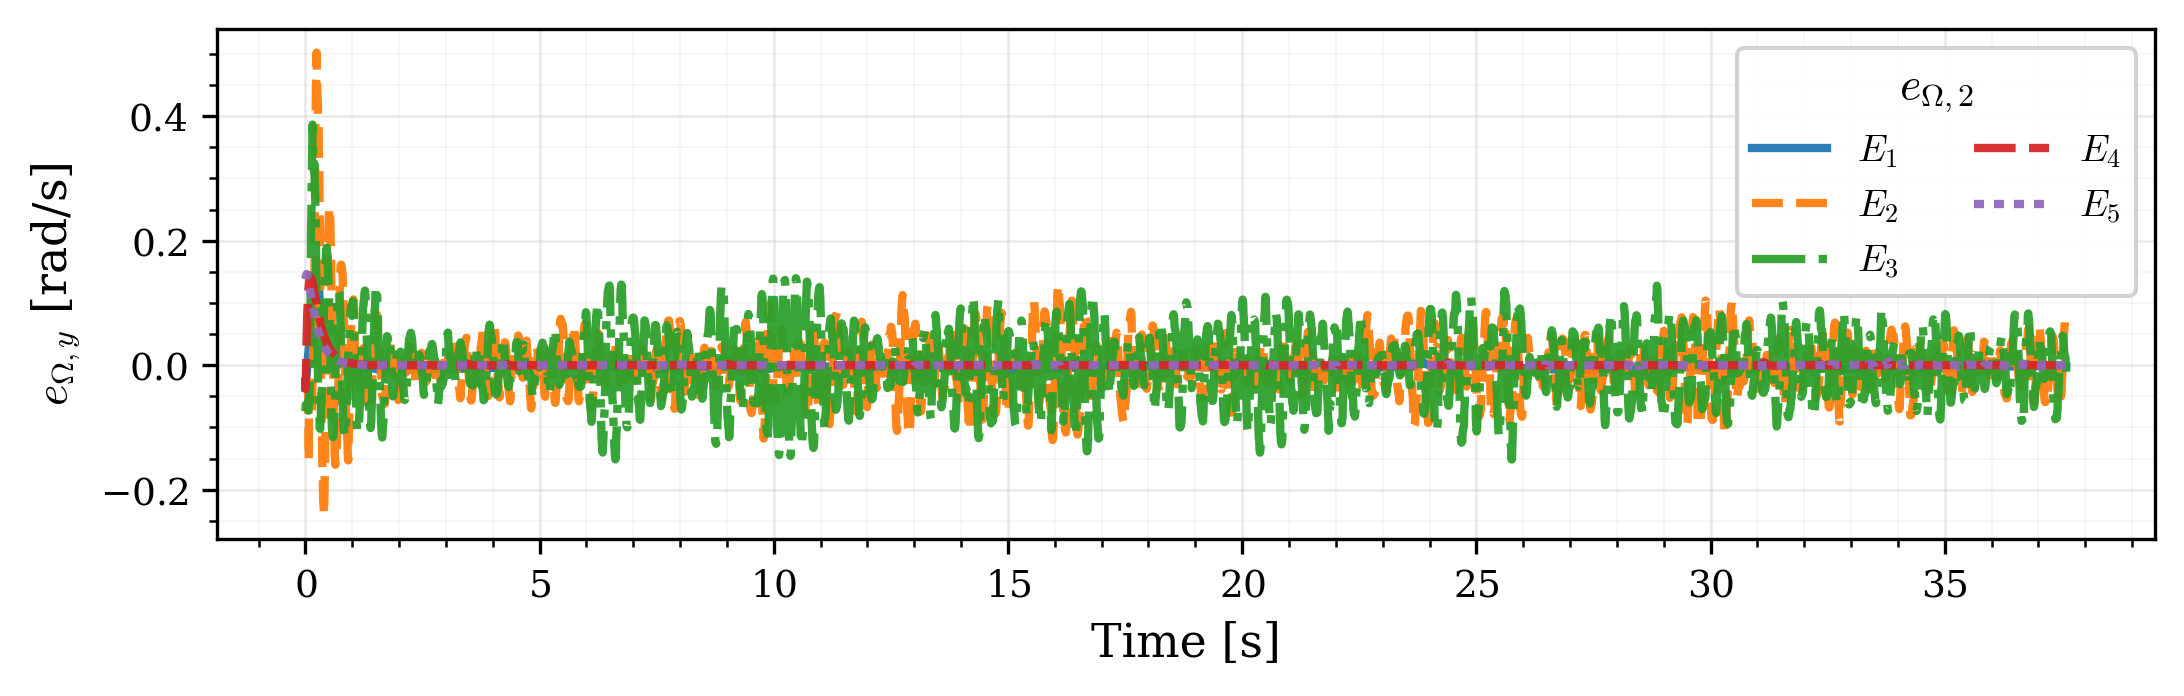
\includegraphics[width=\linewidth]{experiment_plots/error_angular_velocity_component_y.png}\caption{$e_{\Omega,2}(t)$.}\end{subfigure}
    \\
    \begin{subfigure}{\textwidth}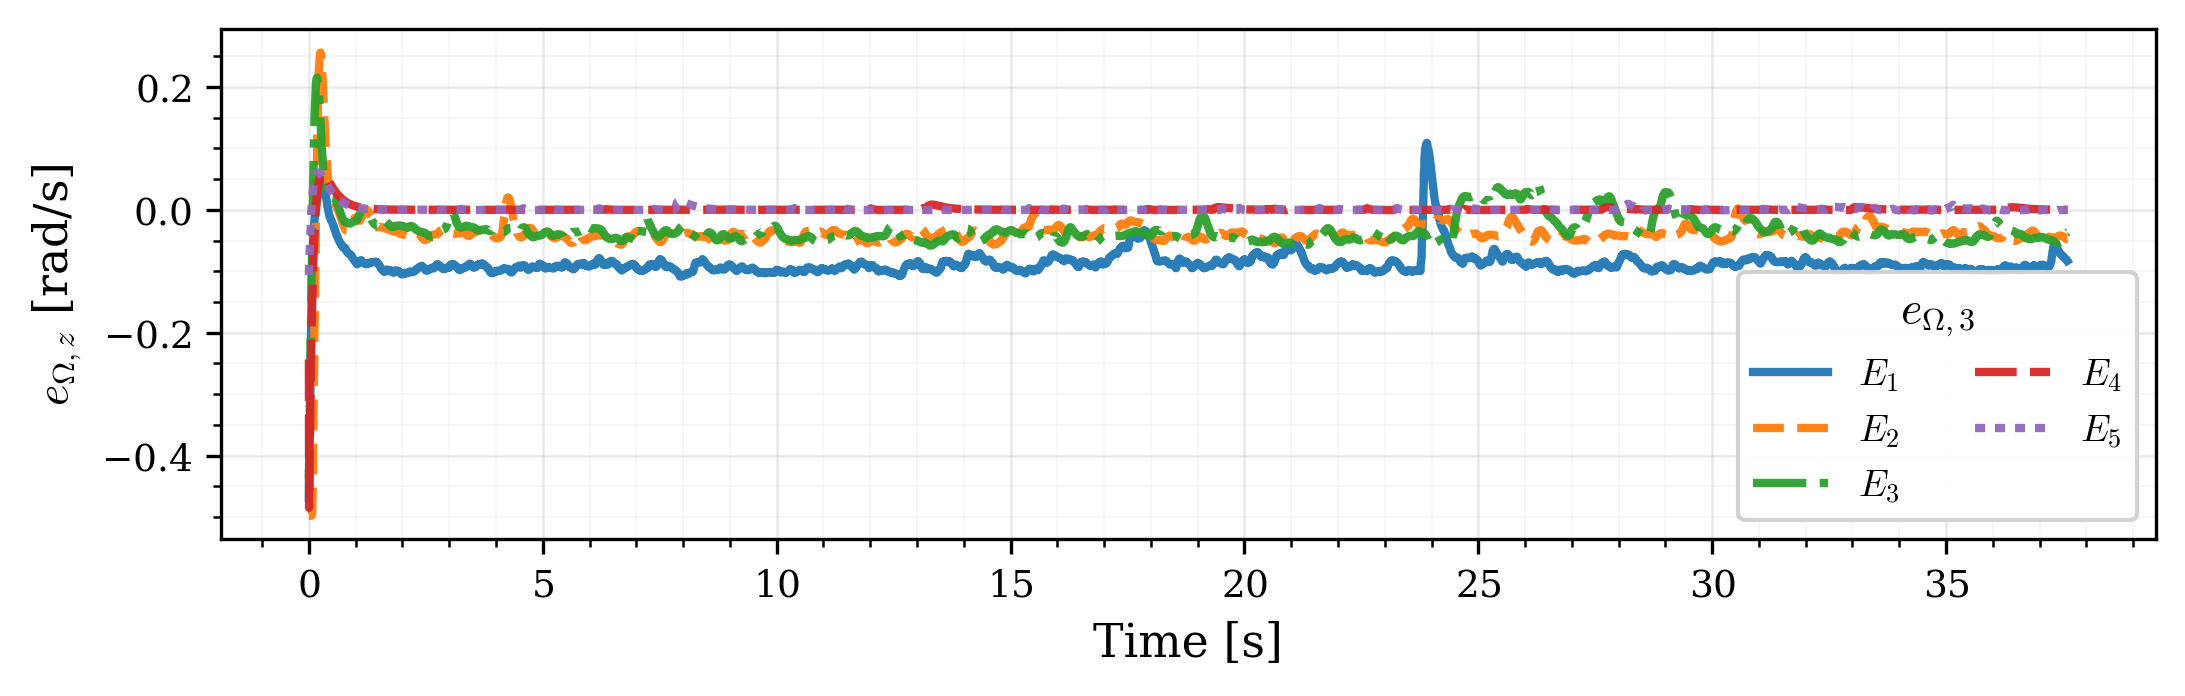
\includegraphics[width=\linewidth]{experiment_plots/error_angular_velocity_component_z.png}\caption{$e_{\Omega,3}(t)$.}\end{subfigure}
    \caption{Per-body-axis components of the angular-velocity error vector $e_\Omega$.}
    \label{fig:app-error-eOm-axes}
\end{figure}

\subsection{Per-Axis Angular-Acceleration Tracking}
\begin{figure}[H]
    \centering
    \begin{subfigure}{\textwidth}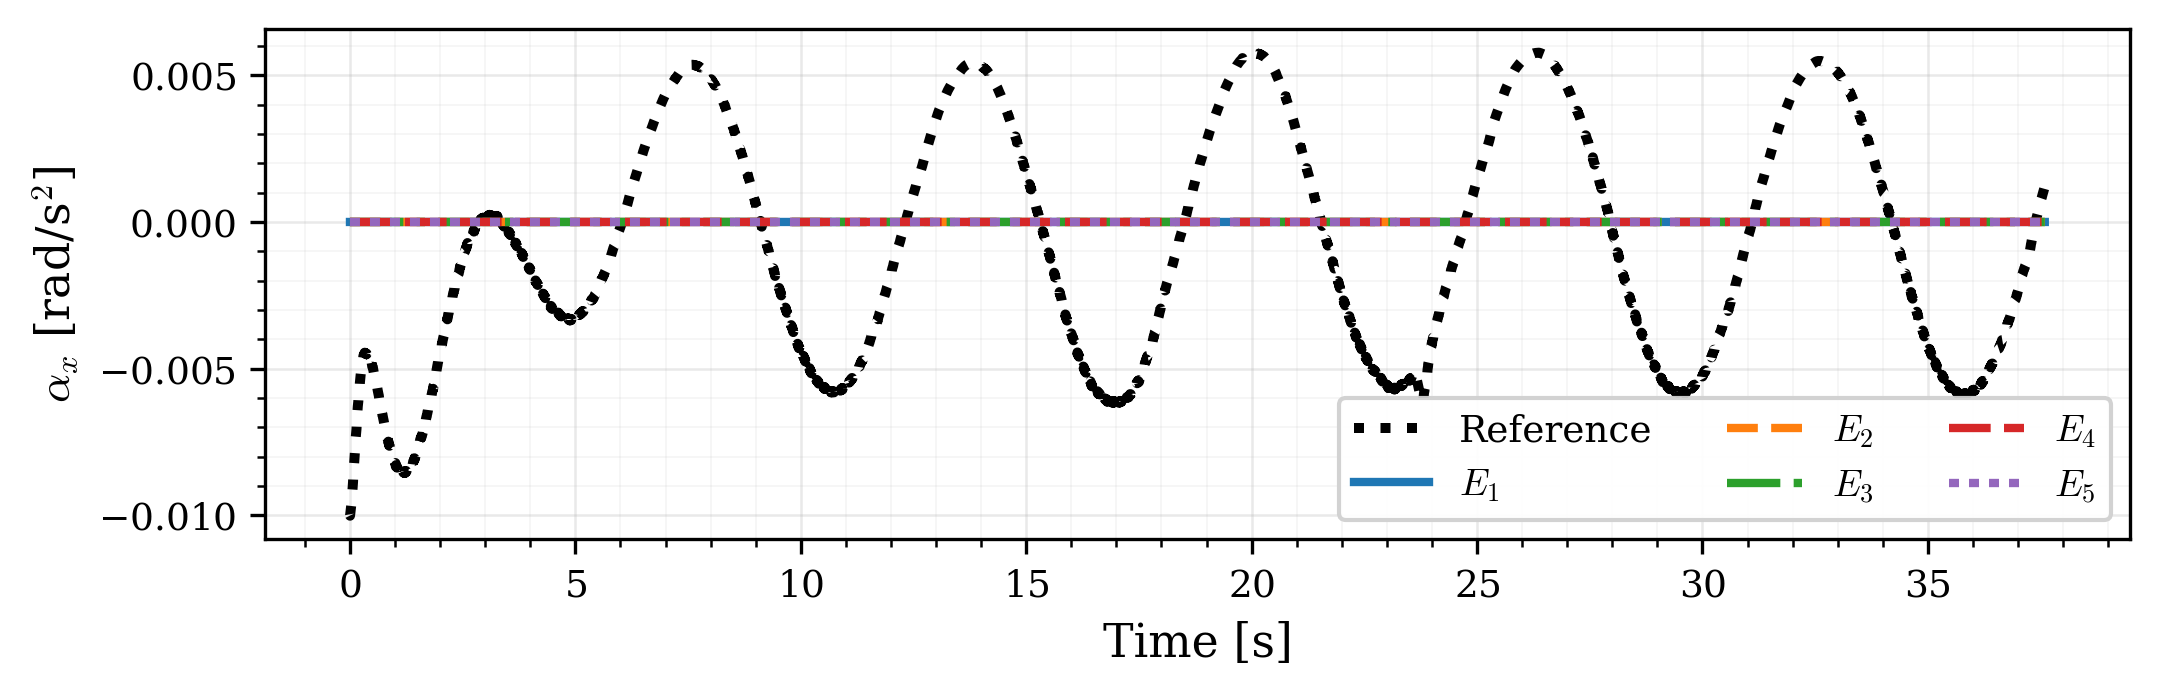
\includegraphics[width=\linewidth]{experiment_plots/tracking_angular_acceleration_x.png}\caption{$\dot\Omega_x(t)$.}\end{subfigure}
    \\
    \begin{subfigure}{\textwidth}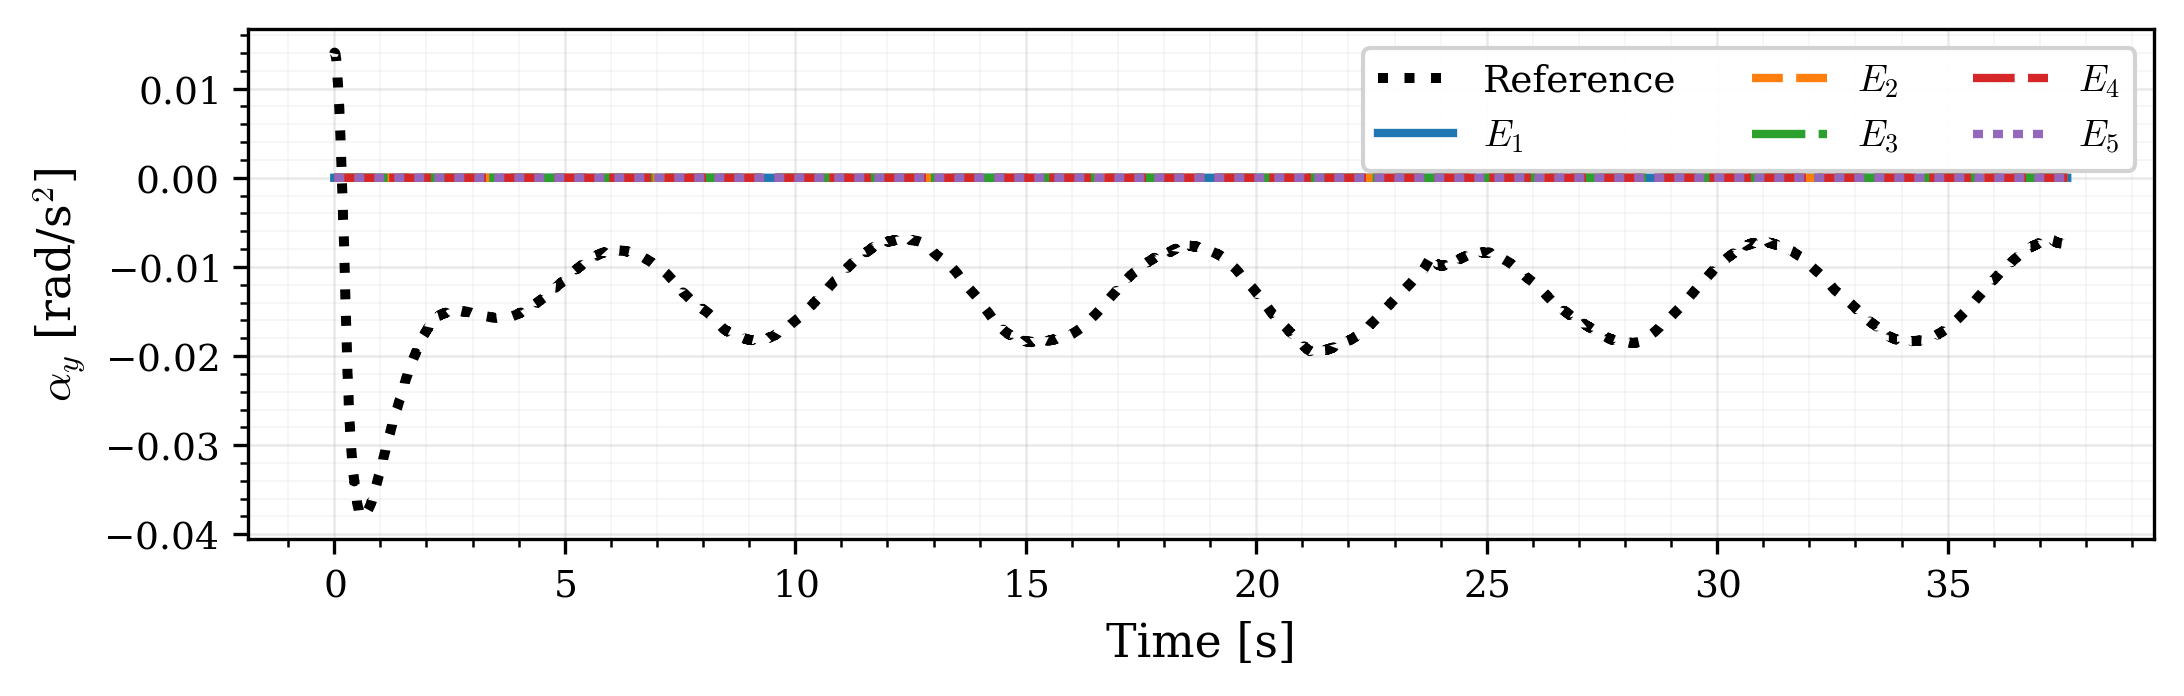
\includegraphics[width=\linewidth]{experiment_plots/tracking_angular_acceleration_y.png}\caption{$\dot\Omega_y(t)$.}\end{subfigure}
    \\
    \begin{subfigure}{\textwidth}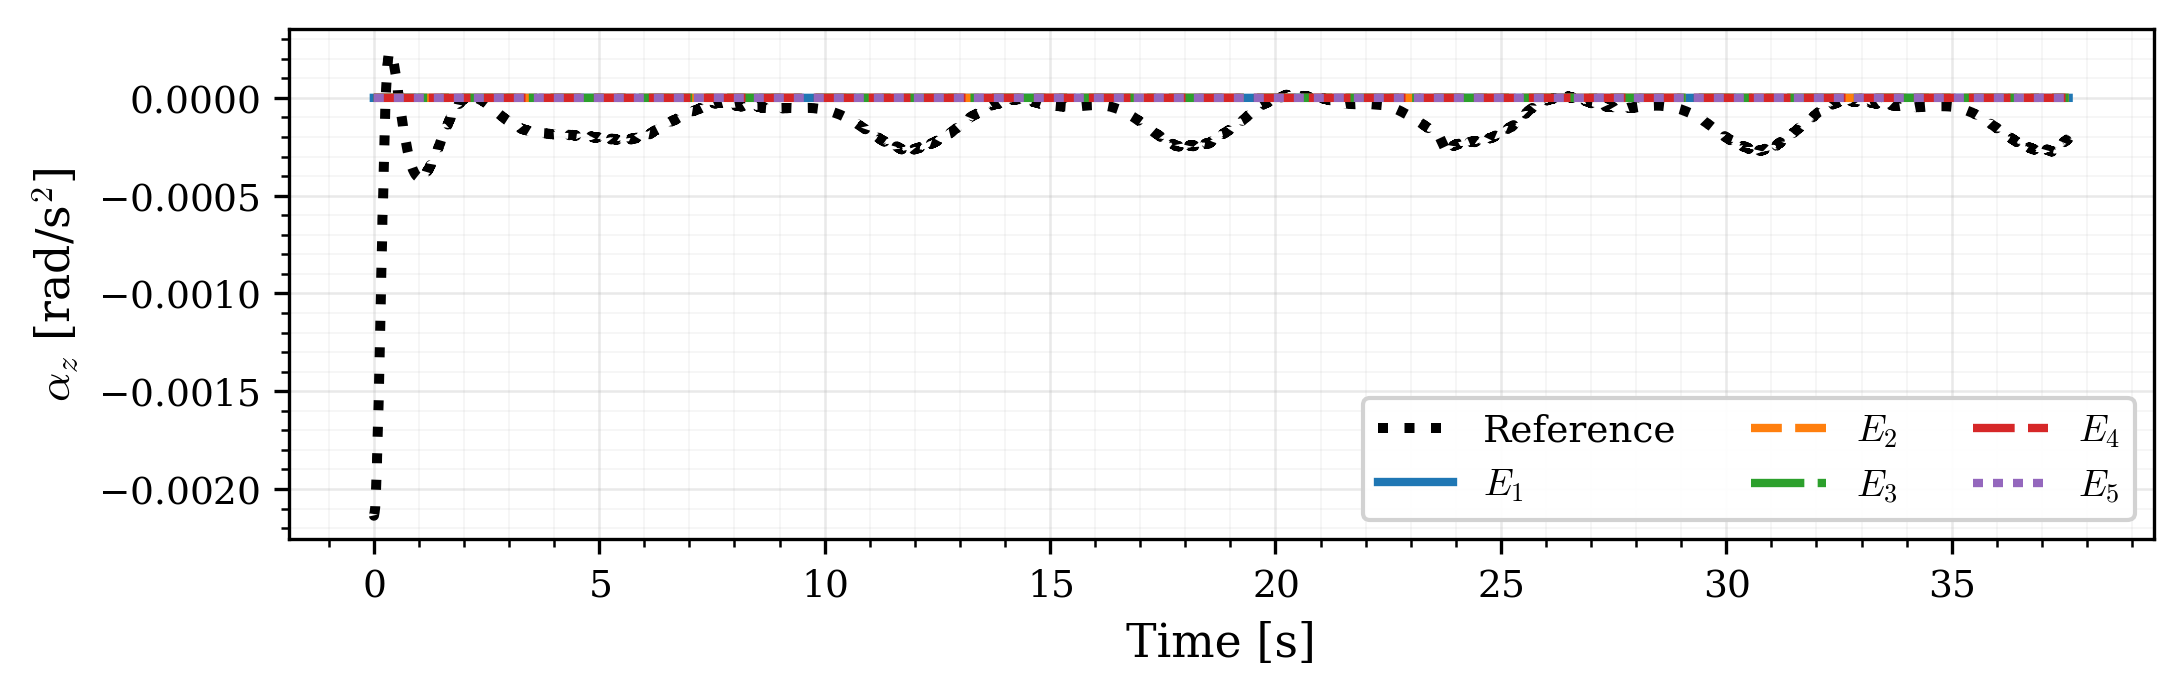
\includegraphics[width=\linewidth]{experiment_plots/tracking_angular_acceleration_z.png}\caption{$\dot\Omega_z(t)$.}\end{subfigure}
    \caption{Per-body-axis angular-acceleration tracking.}
    \label{fig:app-tracking-alpha}
\end{figure}

\subsection{Angular-Acceleration Errors}
\begin{figure}[H]
    \centering
    \begin{subfigure}{\textwidth}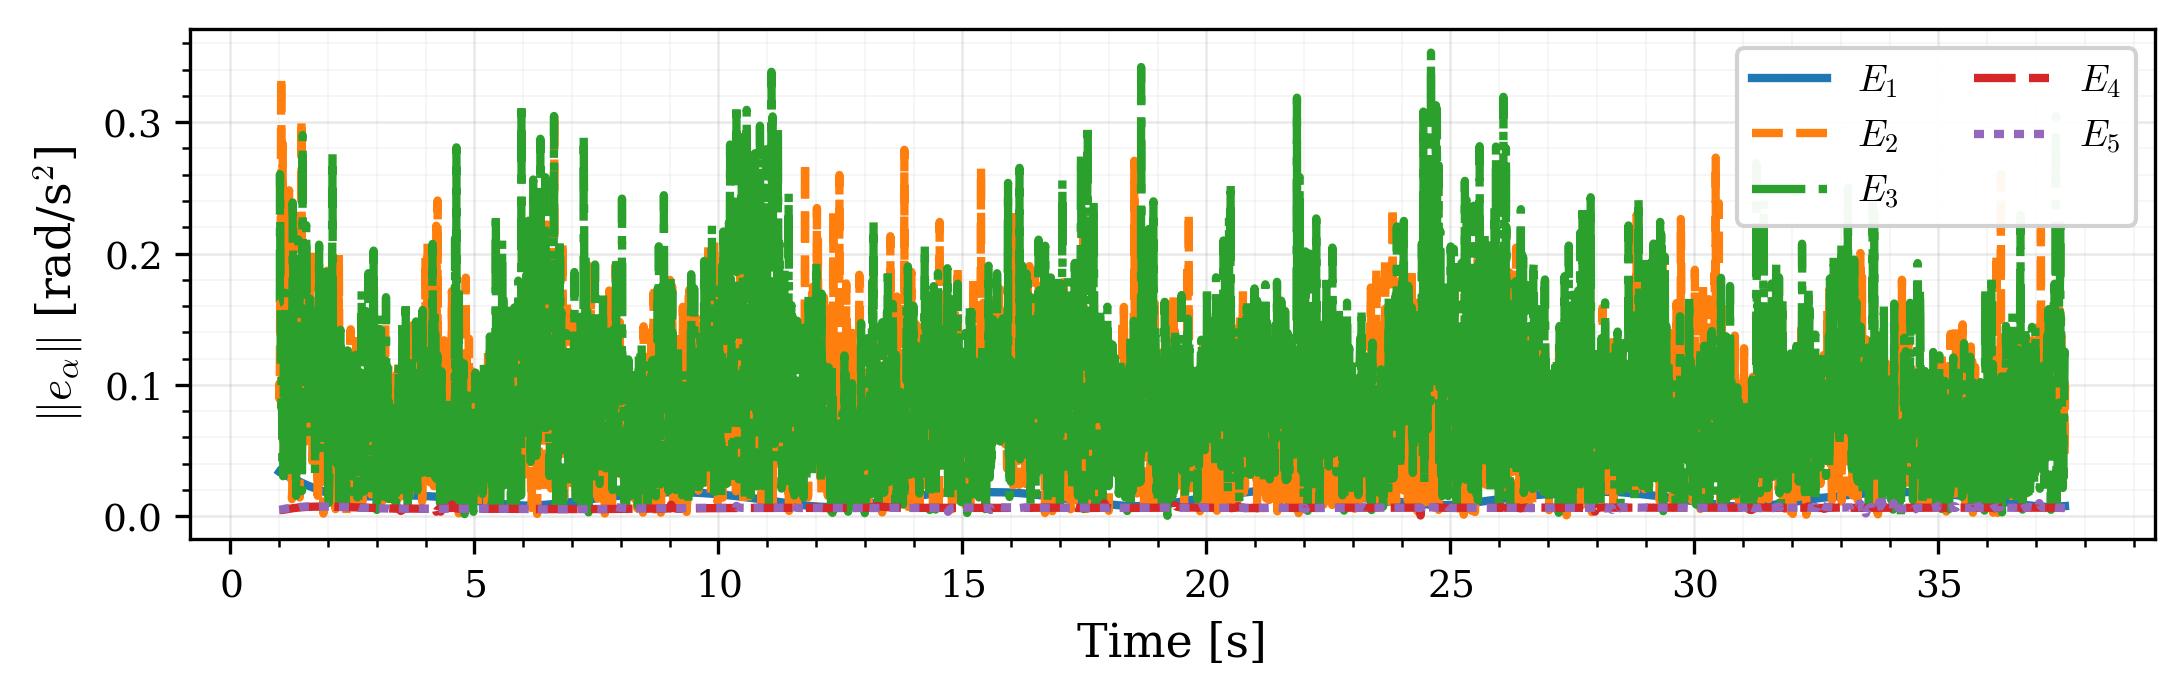
\includegraphics[width=\linewidth]{experiment_plots/error_angular_acceleration.png}\caption{Angular-acceleration-error norm $\|\dot\Omega - \dot\Omega_d\|(t)$.}\end{subfigure}
    \\
    \begin{subfigure}{\textwidth}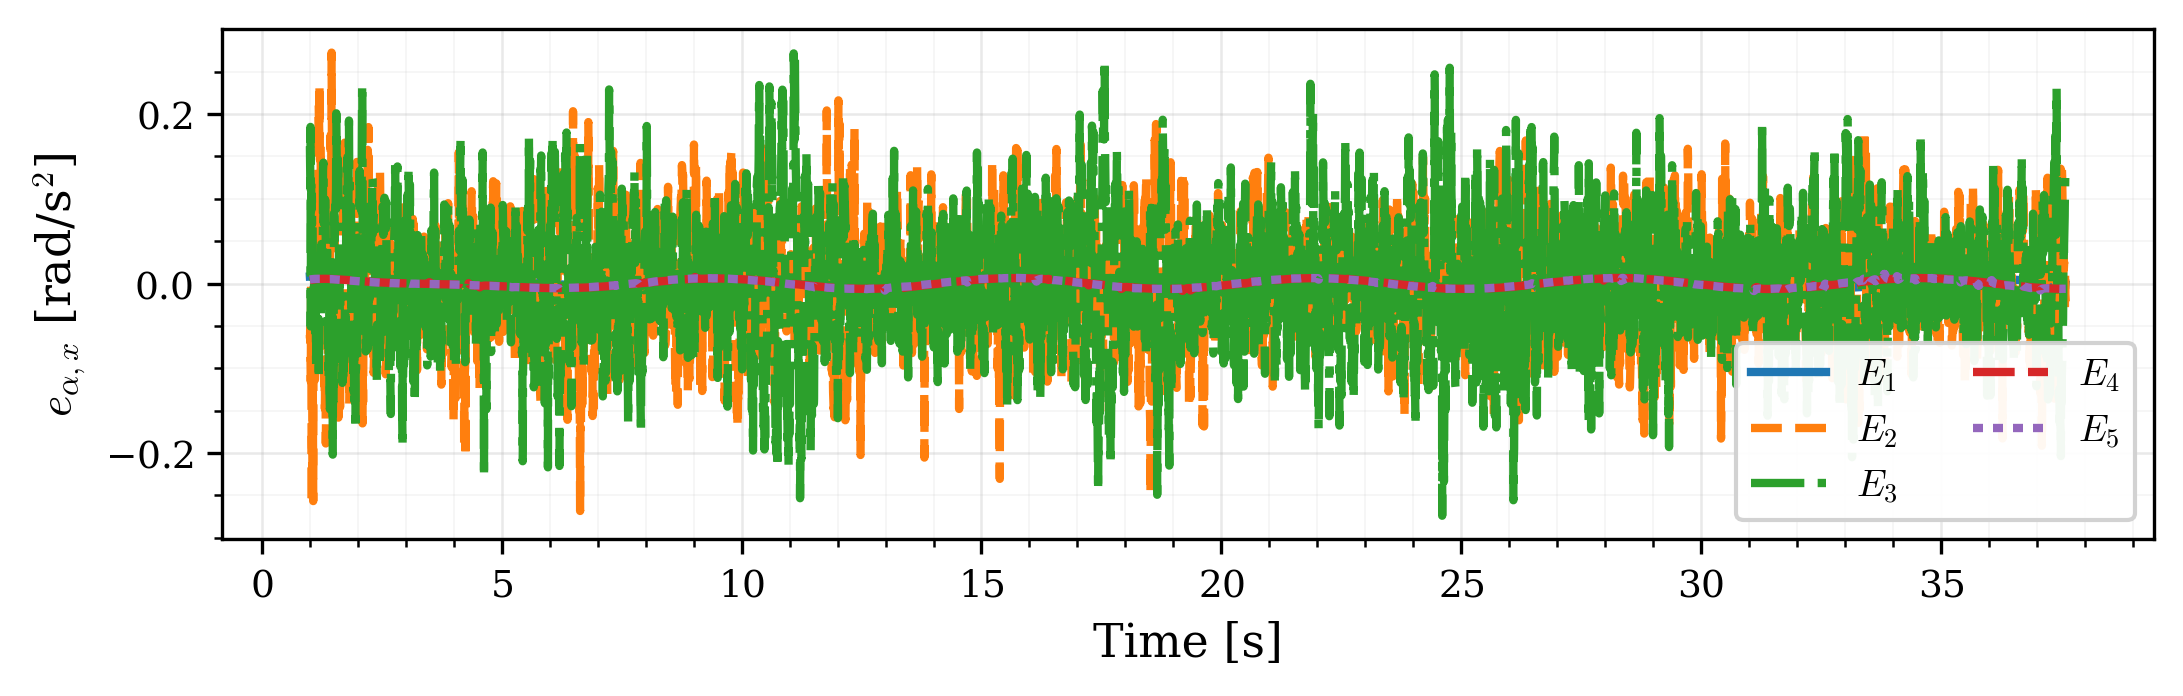
\includegraphics[width=\linewidth]{experiment_plots/error_angular_acceleration_x.png}\caption{$x$-component.}\end{subfigure}
    \\
    \begin{subfigure}{\textwidth}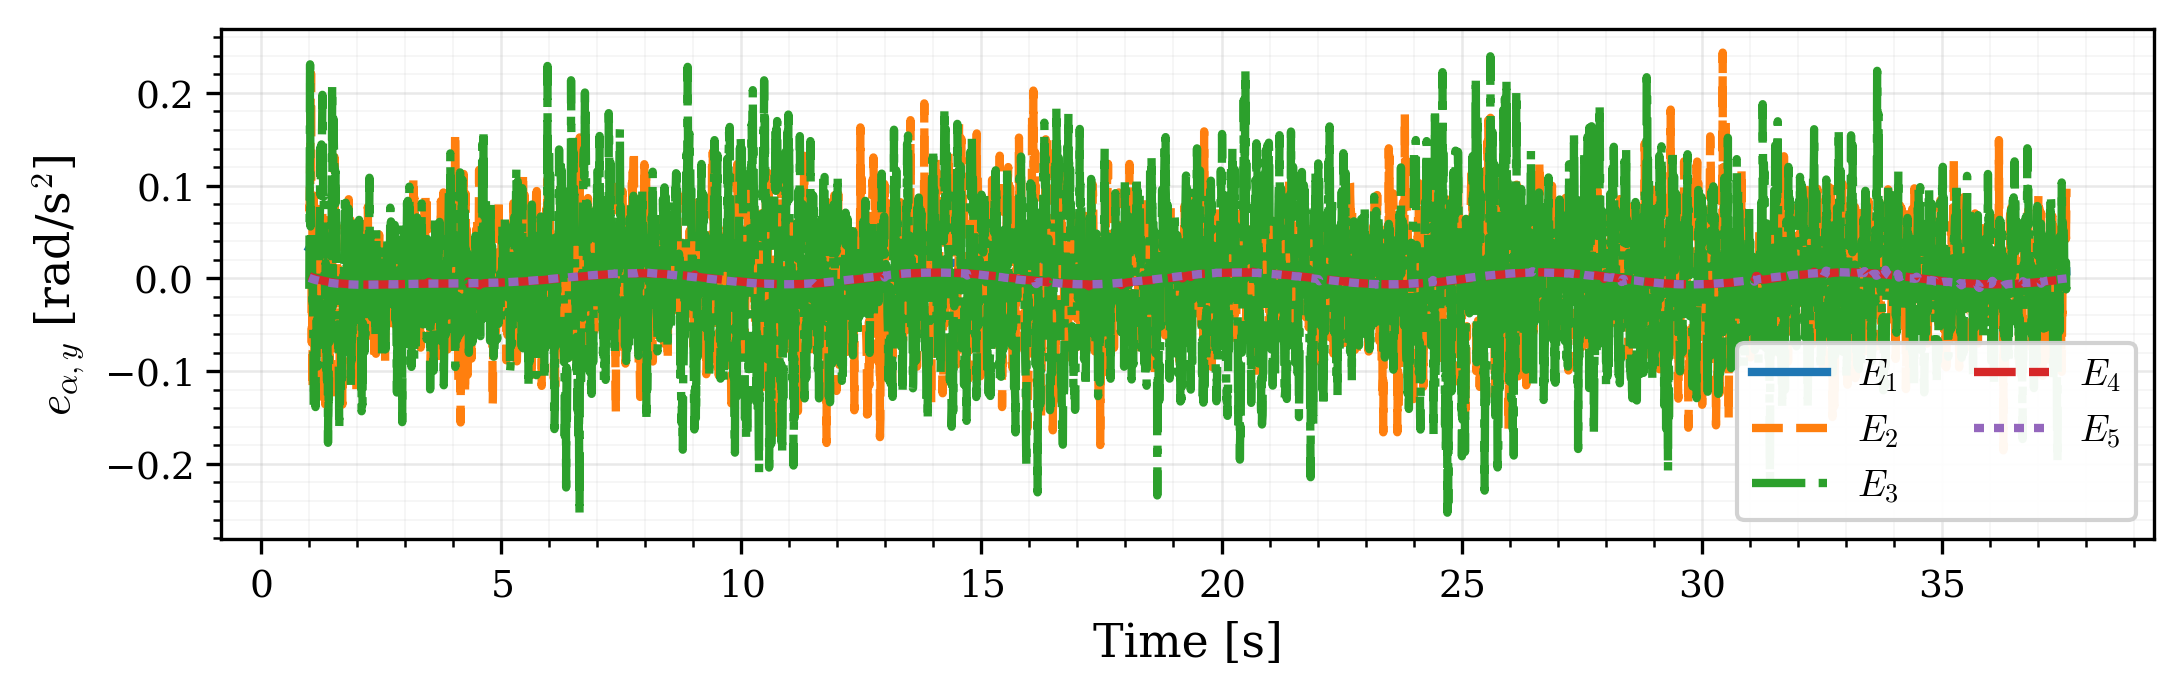
\includegraphics[width=\linewidth]{experiment_plots/error_angular_acceleration_y.png}\caption{$y$-component.}\end{subfigure}
    \\
    \begin{subfigure}{\textwidth}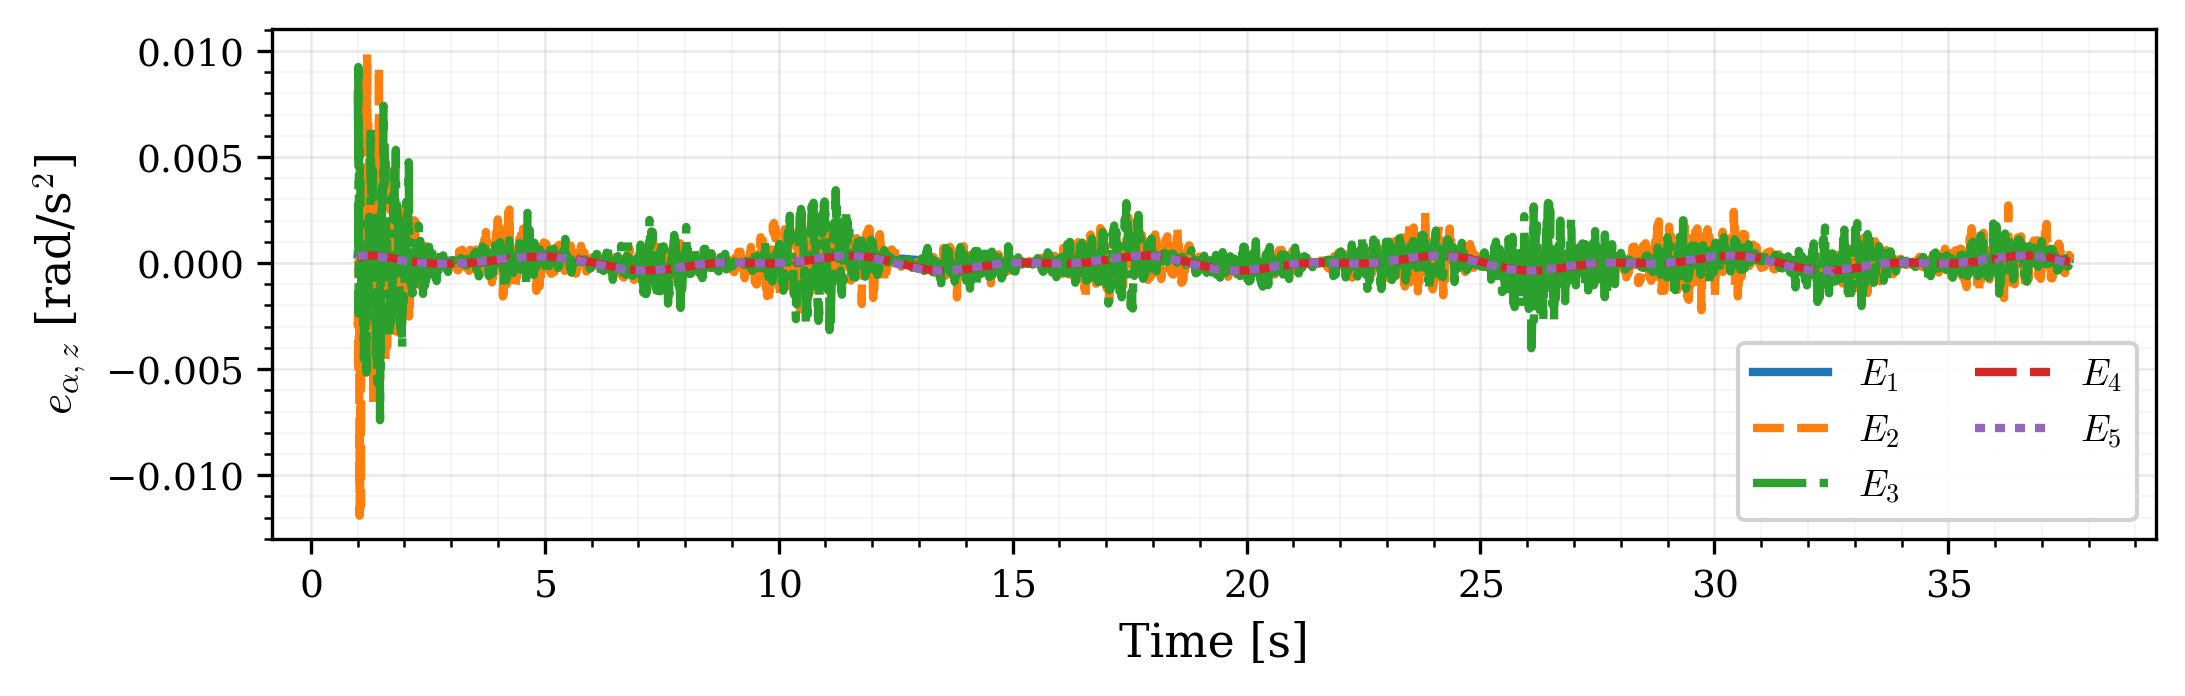
\includegraphics[width=\linewidth]{experiment_plots/error_angular_acceleration_z.png}\caption{$z$-component.}\end{subfigure}
    \caption{Angular-acceleration tracking errors. The norm is dominated by short transients at the start of the trajectory; the steady-state behaviour is most informative in the per-axis breakdown.}
    \label{fig:app-error-alpha}
\end{figure}

\end{document}